\documentclass[dvipsnames, 12pt]{book}
\usepackage[font=small,labelfont=bf]{caption}
\usepackage[b5paper,top=2cm, bottom=2cm, left = 2.5cm, right=2cm]{geometry}

\usepackage[
backend=biber,
style=nature,
sorting=none]{biblatex}
\usepackage{etoolbox}
\usepackage{mathtools}
\usepackage{amsthm}
\usepackage{amstext}
\usepackage{nicefrac}
\usepackage{algorithm}
\usepackage{algpseudocode}
\usepackage{listings}
\usepackage{pxfonts}
\usepackage{pdfpages} 
\usepackage{graphicx}
\usepackage{tgtermes}
\usepackage{titlesec}
\usepackage{url}
%\usepackage{breakurl}
%\def\UrlBreaks{\do\/\do-\do\.}

\usepackage[UKenglish]{babel}
\usepackage{rotating} % to rotate figures with sideways environment
\usepackage{framed}
\usepackage{caption}
\usepackage{soul} % for hl command
\usepackage{multirow}
\usepackage[xindy,toc,acronym,nonumberlist]{glossaries} % for acronyms
\usepackage{ifthen}
\usepackage{booktabs}
\usepackage{longtable}
\usepackage{setspace}


%\usepackage{color}
%\usepackage{tgtermes}
%\usepackage{titlesec}

\newlength{\mytitlewidth}
\definecolor{chaptergrey}{rgb}{0.7,0.7,0.7}
\AtBeginDocument{
  \settowidth{\mytitlewidth}{\normalfont\fontsize{60}{0}\selectfont\chaptername}
}

\newcommand{\setchaptertitle}[1]{\parbox[t]{\mytitlewidth}{\raggedleft#1}}
\newcommand{\setchapternumber}{%
  \fontsize{100}{0}\color{chaptergrey}\selectfont\thechapter}

\titleformat{\chapter}[display]
  {\raggedleft\normalfont\fontsize{60}{0}\selectfont}
  {\filleft\setchapternumber}
  {15pt}
  {\huge\setchaptertitle}

\input{Subsubsection.tex}
\DeclarePairedDelimiter\abs{\lvert}{\rvert}
\DeclarePairedDelimiter\norm{\lVert}{\rVert}

%\usepackage{listings}
%\usepackage{xcolor}
%\usepackage{etoolbox}
%\usepackage{pxfonts}

\newtoggle{InString}{}% Keep track of if we are within a string
\togglefalse{InString}% Assume not initally in string

\newcommand*{\ColorIfNotInString}[1]{\iftoggle{InString}{#1}{\color{red}#1}}%
\newcommand*{\ProcessQuote}[1]{#1\iftoggle{InString}{\global\togglefalse{InString}}{\global\toggletrue{InString}}}%

\colorlet{punct}{red!60!black}
\definecolor{background}{HTML}{EEEEEE}
\definecolor{delim}{RGB}{20,105,176}
\colorlet{numb}{magenta!60!black}

\lstdefinelanguage{json}{
    basicstyle=\ttfamily,
    numbers=left,
    numberstyle=\scriptsize,
    stepnumber=1,
    numbersep=8pt,
    showstringspaces=false,
    %breaklines=true,
    %frame=lines,
    %
    frame=single,
    breaklines=true,
    postbreak=\raisebox{0ex}[0ex][0ex]{\ensuremath{\color{red}\hookrightarrow\space}},
    alsoletter = {"},
    morekeywords={String},
    emph={String, Real, Integer, Boolean, List},
    emphstyle={\bfseries},
    %
    backgroundcolor=\color{background},
    literate=
      {"}{{{\ProcessQuote{"}}}}{1}% Disable coloring within double quotes
      {'}{{{\ProcessQuote{'}}}}{1}% Disable coloring within single quote
      {0}{{{\ColorIfNotInString{0}}}}{1}
      {1}{{{\ColorIfNotInString{1}}}}{1}
      {2}{{{\ColorIfNotInString{2}}}}{1}
      {3}{{{\ColorIfNotInString{3}}}}{1}
      {4}{{{\ColorIfNotInString{4}}}}{1}
      {5}{{{\ColorIfNotInString{5}}}}{1}
      {6}{{{\ColorIfNotInString{6}}}}{1}
      {7}{{{\ColorIfNotInString{7}}}}{1}
      {8}{{{\ColorIfNotInString{8}}}}{1}
      {9}{{{\ColorIfNotInString{9}}}}{1}
      {:}{{{\color{punct}{:}}}}{1}
      {,}{{{\color{punct}{,}}}}{1}
      {\{}{{{\color{delim}{\{}}}}{1}
      {\}}{{{\color{delim}{\}}}}}{1}
      {[}{{{\color{delim}{[}}}}{1}
      {]}{{{\color{delim}{]}}}}{1},
}

\renewcommand{\lstlistingname}{JSON}

\newcommand{\crparagraph}[1]{\paragraph{#1}\mbox{}\\}

\input{Dedication.tex}

\newcommand{\specialcell}[2][c]{%
  \begin{tabular}[#1]{@{}c@{}}#2\end{tabular}}


\addbibresource{thesis.bib}

\title{Algorithmic and Technical Improvements for Next Generation Drug Design Software Tools}
\date{2013-09-01}
\author{V\'ictor A. Gil Sep\'ulveda}

% allow to add input and output kw in algorithms
\algnewcommand\algorithmicinput{\textbf{Input:}}
\algnewcommand\Input{\item[\algorithmicinput]}
\algnewcommand\algorithmicoutput{\textbf{Output:}}
\algnewcommand\Output{\item[\algorithmicoutput]}

% macro utils
\newcommand{\ignore}[2]{\hspace{0in}#2}
\newcommand{\fittopageimage}[2][]{\includegraphics[width=\linewidth, height=\textheight, keepaspectratio,#1]{#2}}
\newcommand{\calpha}{$C_\alpha$\ }
\newcommand{\angstrom}{$\AA$\ }
\newcommand{\around}{$\sim$}

%\tracingall
\newcommand{\grt}[2]{\lengthtest{#1 pt > #2 pt}}
\newcommand{\strcolor}[1]{\ifthenelse{ \grt{#1}{0.49} \or \grt{-0.49}{#1}}{\textcolor{green}{#1}}{\ifthenelse{\grt{#1}{0.29} \or \grt{-0.29}{#1}}{\textcolor{GreenYellow}{#1}}{\ifthenelse{\grt{#1}{0.09} \or \grt{-0.09}{#1}}{\textcolor{BurntOrange}{#1}}{\textcolor{red}{#1}}}}}

\bibliography{thesis}
\setcounter{secnumdepth}{4}
\setcounter{tocdepth}{4} 


\newacronym{sasa}{SASA}{Solvent-Accessible Surface Area}
\newacronym{rmsf}{RMSF}{Root Mean Square Fluctuation}
\newacronym{rmsd}{RMSD}{Root Mean Square Deviation}
\newacronym{ic}{IC}{Internal Coordinates}
\newacronym{cc}{CC}{Cartesian Coordinates}
\newacronym{mc}{MC}{Monte Carlo}
\newacronym{md}{MD}{Molecular Dynamics}
\newacronym{randd}{R\&D}{Research and Development} 
\newacronym{pele}{PELE}{Protein Energy Landscape Exploration}
\newacronym{idp}{IDP}{Intrinsically Disordered Protein}
\newacronym{fda}{FDA}{Food and Drug Administration}
\newacronym{nme}{NME}{New molecular Entity}
\newacronym{hts}{HTS}{High-Throughput Screening}
\newacronym{vs}{VS}{Virtual Screening}
\newacronym{vhts}{VHTS}{Virtual High-Throughput Screening}
\newacronym{lbvs}{LBVS}{Ligand-Based Virtual Screening}
\newacronym{sbvs}{SBVS}{Structure-Based Virtual Screening}
\newacronym{fep}{FEP}{Free Energy Perturbation (method)} 
\newacronym{pmf}{PMF}{Potential of Mean Force}
\newacronym{mmpbsa}{MM/PBSA}{Molecular Mechanics / Poisson-Boltzmann Surface Area}
\newacronym{pcr}{PCR}{Polymerase Chain Reaction}
\newacronym{dna}{DNA}{Deoxyribonucleic Acid}
\newacronym{rna}{RNA}{Ribonucleic Acid} 
\newacronym{admetox}{ADME/Tox}{Absorption, Distribution, Metabolism, Excretion\\ / Toxicological}
\newacronym{pdb}{PDB}{Protein Data Bank}
\newacronym{nmr}{NMR}{Nuclear Magnetic Resonance}
\newacronym{cpu}{CPU}{Central Processing Unit}
\newacronym{nma}{NMA}{Normal Mode Analysis}
\newacronym{anm}{ANM}{Anisotropic Network Model}
\newacronym{en}{EN}{Elastic Network}
\newacronym{rtb}{RTB}{Rotational-Translational Block}
\newacronym{bnm}{BNM}{Block Normal Mode}
\newacronym{cg}{CG}{Coarse Grain}
\newacronym{opls}{OPLS}{Optimized Potential for Liquid Simulations}
\newacronym{gpu}{GPU}{Graphics Processing Unit}
\newacronym{obc}{OBC}{Onufriev-Bashford-Case}
\newacronym{sgb}{SGB}{Surface Generalized Born}  
\newacronym{amber}{AMBER}{Assisted Model Building with Energy Refinement}
\newacronym{nvt}{NVT}{(constant) Number (of particles), Volume and Temperature}
\newacronym{mmc}{MMC}{Metropolis Monte Carlo}
\newacronym{icnma}{icNMA}{Internal Coordinate Normal Mode Analysis}
\newacronym{ccnma}{ccNMA}{Cartesian Coordinate Normal Mode Analysis}
\newacronym{oop}{OOP}{Object-Oriented Programming}
\newacronym{mic}{MIC}{Many Integrated Core} 
\newacronym{gpgpu}{GPGPU}{General-Purpose computing on Graphics Processing Units}
\newacronym{arm}{ARM}{Advanced RISC (Reduced Instruction Set Computing) Machine}
\newacronym{pca}{PCA}{Principal Component Analysis}
\newacronym{msm}{MSM}{Markov State Model}

%\glsaddall

%\acronymname{Abbreviations}

\makeglossaries
%\renewcommand*\glspostdescription{\dotfill}

\AtEveryBibitem{\clearfield{month}}
\AtEveryBibitem{\clearfield{day}}

\begin{document}
\cleardoublepage% especially in a document where chapters start at right-hand pages

\pagenumbering{gobble}
\begin{titlepage}

\newcommand{\HRule}{\rule{\linewidth}{0.5mm}} % Defines a new command for the horizontal lines, change thickness here

\center % Center everything on the page
 
%----------------------------------------------------------------------------------------
%	HEADING SECTIONS
%----------------------------------------------------------------------------------------

\textsc{\LARGE Universitat de Barcelona}\\[1.5cm] % Name of your university/college
\textsc{\Large Facultat de Farm\`acia}\\[0.5cm] % Major heading such as course name

%----------------------------------------------------------------------------------------
%	TITLE SECTION
%----------------------------------------------------------------------------------------
\vspace{2.5cm}
%\HRule \\[0.4cm]
{ 
\huge \bfseries Algorithmic and Technical Improvements
for Next Generation Drug Design Software
Tools
}\\[0.4cm] % Title of your document
%\HRule \\[1.5cm]


\vspace{10cm}
V\'ICTOR A. GIL SEP\'ULVEDA, 2016

\vfill % Fill the rest of the page with whitespace

\newpage
\cleardoublepage
\end{titlepage}

\begin{titlepage}

\newcommand{\HRule}{\rule{\linewidth}{0.5mm}} % Defines a new command for the horizontal lines, change thickness here

\center % Center everything on the page
 
%----------------------------------------------------------------------------------------
%	HEADING SECTIONS
%----------------------------------------------------------------------------------------

\textsc{\LARGE Universitat de Barcelona}\\[1.5cm] % Name of your university/college
\textsc{\Large Facultat de Farm\`acia}\\[0.5cm] % Major heading such as course name
\textsc{\large Programa de Doctorat en Biomedicina}\\[0.5cm] % Minor heading such as course title

%----------------------------------------------------------------------------------------
%	TITLE SECTION
%----------------------------------------------------------------------------------------
\vspace{2.5cm}
%\HRule \\[0.4cm]
{ 
\huge \bfseries Algorithmic and Technical Improvements
for Next Generation Drug Design Software
Tools
}\\[0.4cm] % Title of your document
%\HRule \\[1.5cm]
 
Mem\`oria presentada per  V\'ictor A. Gil Sep\'ulveda per \\
optar al t\'itol de doctor per la Universitat de Barcelona
 
%----------------------------------------------------------------------------------------
%	AUTHOR SECTION
%----------------------------------------------------------------------------------------
\vspace{5.5cm}
%\normalsize
%\begin{minipage}{0.4\textwidth}
%\begin{flushleft} \large
%\emph{Autor:}\\
%V\'ictor A. \textsc{Gil} % Your name
%\end{flushleft}
%\end{minipage}
%~
%\begin{minipage}{0.4ºtextwidth}
%\begin{flushright} \large
%\emph{Director:} \\
%Dr. V\'ictor \textsc{Guallar} % Supervisor's Name
%\end{flushright}
%\end{minipage}\\[4cm]

%----------------------------------------------------------------------------------------
%	DATE SECTION
%----------------------------------------------------------------------------------------

%{\large \today}\\[3cm] % Date, change the \today to a set date if you want to be precise

%----------------------------------------------------------------------------------------
%	LOGO SECTION
%----------------------------------------------------------------------------------------


\includegraphics[width=\textwidth]{logos}\\[1cm] % Include a department/university logo - this will require the graphicx package
 
%----------------------------------------------------------------------------------------

\vfill % Fill the rest of the page with whitespace

\newpage
\cleardoublepage
\end{titlepage}

\begin{dedication}
A mi madre, mi padre y\\ mi hermano\\
\smallskip
A Marghe
\end{dedication}

\newpage
%Acknowledgments
\begin{spacing}{1.5}
\chapter*{Agradecimientos}% for the actuall unnumbered heading
\thispagestyle{empty}% or plain etc.

El doctorado es un largo viaje. Un viaje de descubrimiento cient\'ifico, y tambi\'en de descubrimiento personal. Y, en contra de lo que algunos puedan pensar, no es un viaje nada f\'acil. Afortunadamente, a lo largo de su periplo, el viajero encuentra personas que le gu\'ian, le abren caminos y le dan apoyo. Quisiera dedicar estas l\'ineas a esas personas.

Me gustar\'ia empezar agradeciendo al Dr. V\'ictor Guallar, mi supervisor, el haberme dado la oportunidad sin la cual nada de esto hubiera sido posible. Mi m\'as sincera gratitud a las dem\'as personas que me han permitido conocer un poco m\'as el mundo y como se trabaja fuera de Espa\~na, especialmente: al Dr. Juan Cort\'es, del LAAS-CNRS, por haberme acogido en mi primera estancia en el extranjero; al Dr. Scott Callaghan, uno de los organizadores del programa \textit{HPC summer school}, al cual le debo el haber ``cruzado el charco'' por primera vez; y al Dr. Anders Hogner por acogerme en su grupo de investigaci\'on en AstraZeneca y haberme hecho sentir como si fuera uno m\'as del equipo.   


Todo viaje largo se disfruta m\'as en buena compa\~n\'ia. Considero haber tenido mucha suerte en ese aspecto, tanto en el terreno personal como en el laboral. Durante todos estos a\~nos, he podido gozar de la compa\~nia de mis colegas del Barcelona Supercomputing Center. Con ellos he compartido reflexiones (a veces cient\'ificas), alegr\'ias y penas. Ser\'ia dif\'icil escribir los nombres de todas las personas que he conocido y aprecio sin que la memoria me acabara traicionando. Gracias a todos! 


Agradezco tambi\'en el apoyo incondicional de mi madre, mi padre, y mi hermano. Ellos no han escrito una tesis doctoral, pero sin duda tienen madera para hacerlo. Finalmente, doy las gracias a la Dra. Margherita Taffarel, que ha recorrido conmigo este camino. Su excelente trabajo contrarreloj ha ayudado a que esta obra sea mucho mejor de lo que podr\'ia haber sido.

A todos, much\'isimas gracias.

Coraggio!!

\begin{flushright} 
Sant Cugat, 11 de Abril 2016
\end{flushright} 


\end{spacing}

\frontmatter
\newpage

\tableofcontents
\newpage

\addcontentsline{toc}{chapter}{\listfigurename}
\listoffigures
\newpage

\addcontentsline{toc}{chapter}{\listtablename}
\listoftables
\newpage

\printglossary[type=\acronymtype,title=Abbreviations]
\newpage
\glsaddall

\mainmatter

\linespread{1.25}
\chapter{Introduction}

\ignore{\hl{General: - Coherencia tiempos verbales - Coherencia protein-ligand - Asegurarse que siempre es
PELE++ (post rewrite) }}

Human biology seats in a weak equilibrium. The breakdown of this homeostasis, whether it is because of external agents or deficiencies in the internal regulations, produces illness and death. Therefore, it is not surprising that, throughout its history, humankind has always been looking for treatments and medicines to fight disease. 
Today, more than ever before, we need to keep perfecting health methods. Industrial excesses and lax laws are creating a hostile environment that affects us directly or through the food chain in unexpected ways. Also, the same advances that have allowed the rise of the world's population life expectancy \cite{who_world_????} are being put to the test to cure the increasing number of aging-related illnesses that reduce our quality of life.

\section{The innovation crisis in pharmaceutical industry}

Nowadays, the role of discovering and manufacturing new and better drugs is being played mainly by the pharmaceutical industry. With a 3.9\% of the gross value added in manufacturing worldwide in 2011 \ignore{\hl{an updated document (2015) exists, but it only contains info up to 2012 (good maps for defense); Gross Value Added es equivalente al PIB}} \cite{ostwald_measuring_2013}, more than 690,000 direct employees in Europe (2013) \cite{efpia_pharmaceutical_2014} and more than 810,000 in the United States of America (USA) (2013) \cite{phrma_2015_2015}, its economical importance is out of doubt. Most big pharmaceutical companies have good financial results and are able to attract investors. However,these good results are mainly because of their incremental innovation model, that is, their ability to improve old products \cite{kristopher_hult_should_????}. This is an efficient strategy, since it can help milden the profit loss coming from expiring patents at a time when consumers tend to buy generics over brand name drugs\footnote{The balance increased from 49\% in 2000  to 88\% in 2013 \cite{phrma_2015_2015}.}. 

However, if we focus on an innovation indicator like the number of NMEs (New Molecular Entities) approved every year by the USA's Food and Drug Administration\footnote{ All data refers to USA agencies unless otherwise stated.}, the pharmaceutical industry does not look so  prosperous. The number of approved NMEs has been very low during the last decade (with an average of 24 per year \cite{cder_2013_2014}).This is a matter of concern, since , the cost of marketing one of these drugs has increased three times in the same amount of time. Also, the drug development time span has not shortened and it usually lasts 15 years \cite{dimasi_price_2003}, but can exceed 30 years \cite{goozner_800_2004}. The discovery of a single NME is becoming more difficult and costly, and the revenues returned from them rarely exceed Research and Development (R\&D) investments. That is why, currently, the pharmaceutical industry is considered to be faced with a deep innovation crisis.

\subsection{Possible causes of the crisis}

	Numerous efforts have been made to understand the causes of this crisis in order to improve R\&D efficiency and effectiveness. From what is known, the main problem is not the lack of investments, since the annual spending in R\&D has been around \$40-\$50 billion \cite{phrma_2015_2015, paul_how_2010} during the last ten years. Indeed pharmaceutical companies reinvest a 12.4 per cent of gross domestic sales on R\&D, of which 9.3 to 12.4\% (1.2 / 2.4\% of total) go to fundamental research \cite{light_demythologizing_2011}.

\begin{figure}
\fittopageimage{NMECost}
\caption{Cost and time needed to develop and market one NME (including failures). Cost data were obtained from (in plot order) \cite{mestre-ferrandiz_rd_2012} \cite{phrma_2015_2015} \cite{dimasi_price_2003} \cite{tibco_transforming_????} \cite{peter_gwynne_pharmaceutical_????} \cite{tibco_transforming_????}  \cite{paul_how_2010} \cite{phrma_2011_2011} \cite{oconnor_football_????} \cite{dimasi_cost_2015} \cite{mullin_cost_????}. Time data were obtained from \cite{dreyfus_keeping_????} \cite{dreyfus_keeping_????} \cite{peter_gwynne_pharmaceutical_????} \cite{paul_how_2010}.}
\label{fig:drug_cost}
\end{figure}

Possible causes of the innovation problem include \cite{hughes_innovation_2007}:

\begin{itemize}

\item The increasingly difficult requirements from regulatory agencies to accept new drugs. New standards of safety make clinical trials longer and more costly.

\item The ``saturation of low hanging fruits'' theory, which says that pharmaceutical industry has already discovered all that is possible with our current knowledge.

\item R\&D teams give a sharp focus to revolutionary instead of evolutionary technologies. For instance, the use of genomics-based candidates was so promising that was prioritized over clinically validated drug targets. Still, the repercussions of including revolutionary technologies in pharmaceutical pipelines are not always negative. For example PCR\footnote{Polymerase Chain Reaction} (1983) for DNA\footnote{Deoxyribonucleic acid} replication or gene chips for RNA\footnote{Ribonucleic acid } in the early 1990s allowed researchers to perform more and faster experiments.  

\item Pharmaceutical companies are extremely big, and they spend great amounts of resources on non-productive work.
\end{itemize}

\subsection{Solutions from the pharmaceutical industry }

Pharmaceutical companies have reacted to this situation immediately in order to improve the outcome of their R\&D investments. One of the consequences has been the forge of strategic alliances (especially with biotechnology firms) or even company mergers\footnote{ For instance, the two giants Pfizer and Allergan, have entered into a merger agreement (announced on the 23th of November of 2015), after several hostile takeover bids to AstraZeneca in 2014.}. The industry has also changed its marketing strategies in an attempt to overcome this delicate situation. For instance focusing on rare diseases, or opting for chronic diseases instead of acute diseases make clinical trials more challenging but give good economic results in the long term. 
Finally, drug repurposing seems a good solution as it can reduce the costs of bringing a drug to the market by almost 40\% \cite{chong_new_2007}.

Special attention has been paid to boosting the efficiency of the drug discovery pipeline steps, as this has direct repercussion on the final cost and on the time invested on the drug . For instance, an outsourcing of early steps such as screening, lead identification or lead optimization has shown to decrease the total costs noticeably. Interestingly, if several companies share the same service providers, they will act as  knowledge and expertise exchange nodes, which seems to be a very beneficial side effect in such a hermetic environment . 

\section{The drug discovery pipeline }

The drug discovery pipeline can be divided into two consecutive main phases. In the first one, the aim of researchers is to understand the illness and find a molecule that can cure it (or, at least, improve its symptoms). During the second main phase, which starts right after regulatory agency clearance, the drug is tested in human patients. 

Nowadays Bioinformatics and Computational Biology software play an important role in the discovery process\footnote{The success of Shr\"{o}dinger is a good example of the increasing importance of computational methods in drug discovery. In 2015 they signed a \$120M deal with Sanofi (with tasks including target analysis, validation, lead identification and lead optimization). More recently (2016) they have entered a research collaboration agreement with Pfizer.}. It is hard to quantify the  impact of software on efficiency because, unfortunately, there are few studies on this topic. However, it is quite obvious that the improvements made on this software would also lead to improvements in the overall effectiveness of the pipeline. 

The phases of the pipeline are:
\begin {enumerate}
\item Discovery process
\begin {description}
\item [Pre-discovery] The goal of this phase is to study a disease in order to understand its causes. This phase is usually neglected in pharmaceutical industry reports because of two main factors. First, the time and budget needed are often very variable and this phase generally contributes to drug discovery in the long term. Second, this kind of research is usually performed at non-corporate tax-funded institutions, such as universities or government research centers, and do not have a direct impact on companies budgets. Fostering basic research and the technology transfer between these institutions and the industry is of utmost importance in order to shorten the time of this phase.
\item [Target identification] During this phase, a druggable molecule involved in the disease, usually a protein, is searched . Improvements in this stage come from the use of gene chips and bioinformatics techniques, as well as proteomics \cite{cutler_proteomics_2015}. The sequencing of the human genome also seemed to be an abundant source of drug targets \cite{ grenet_significance_2001, hopkins_druggable_2002}, but, in general, it has not met the initial expectations yet  \cite{garnier_rebuilding_????}. 
\item [Target validation] During this process, the previous target is tested in single cells and animal models. In-vitro validation can be performed by disrupting target expression through the use of  gene knockouts. 
\item [Lead identification] At this point, researchers look for the chemical leads (small drug-like molecules capable of altering the function of the target proteins) and early pharmacokinetics tests (ADME/Tox\footnote{Absorption, Distribution, Metabolism, Excretion and Toxicological}) are performed. This includes the target-to-hit phase, a preliminary screening to filter non-active compounds, and the hit-to-lead phase, a secondary screening where the compounds with the higher potential to become a drug are chosen. High-throughput screening (HTS) and virtual high throughput screening (VHTS) supported by chemoinformatics seem to help speed up this phase. 
\item [Lead optimization] Leads are further optimized to act as a non-toxic therapeutic drug. Rational drug design and combinatorial chemistry work can be used to improve the  properties of the drug candidate.
\item [Preclinical testing] Drug toxicity is determined using in-vitro and in in-vivo (animal models) experiments.
\end {description}

\item Development process
\begin{description}
\item [Phase 1 clinical trial] Initial tests in healthy volunteers (20-100).
\item [Phase 2 clinical trial] Test in a small group of patients (100-500).
\item [Phase 3 clinical trial] Safety and efficacy tests in a large group of patients (1000-5000).
\item [Phase 4 monitoring] After this steps the drug is commercialized, but it is still monitored in search of possible undocumented side effects.
\end{description}
\end {enumerate}

Several new technologies have been used to lower the cost and time required for clinical trials. Genomics, for instance, would allow subdividing patients according to their drug response, and pharmacogenetics and expression pharmacogenomics can enhance the predictions of patient's drug response by analyzing their DNA variability or determining the levels of gene expression.
The use of collaborative management software in clinical trials has shown to have positive effects on the efficiency as it makes researchers less prone to commit errors.

\begin{sidewaysfigure}
    \centering
    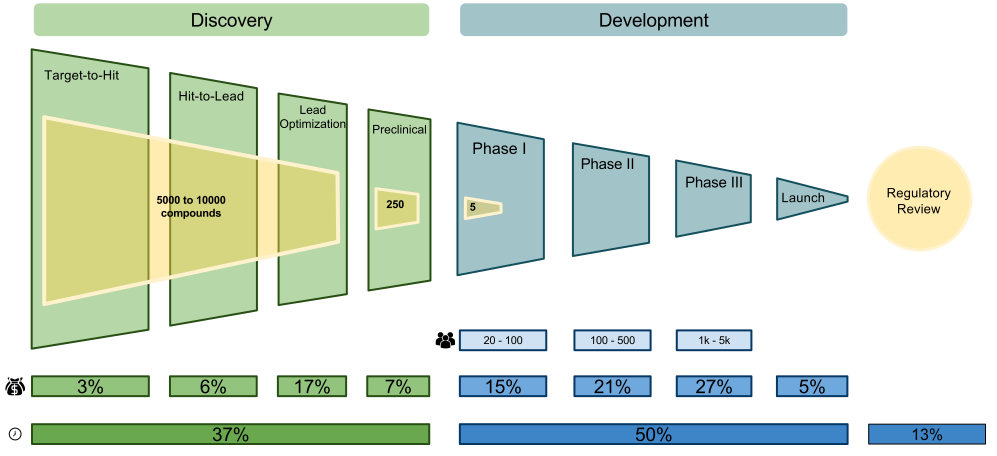
\includegraphics[width=\textwidth,height=\textheight,keepaspectratio]{DrugDevPipeline.pdf}    
    \caption{Drug discovery pipeline phases (pre-discovery and target identification phases have been omitted). The number of compounds used at each step \cite{efpia_pharmaceutical_2014, phrma_2013_2013}, the number of people involved in the clinical trials \cite{phrma_2013_2013}, the percentage of the total development cost per phase \cite{paul_how_2010}, and the percentage of time invested in each phase \cite{dimasi_cost_2015, light_demythologizing_2011, austin_research_2006} are illustrated.}
    \label{fig:drug_dev_pipeline}
\end{sidewaysfigure}

\section{HTS and VHTS}

The early steps of the pipeline are crucial for the success. Target selection, for instance, is one of the most important determinants of R\&D productivity as an error during this phase can potentially compromise the entire process.  

The lead identification step is a very sensitive point too. This step is often performed using HTS. With this technique, lead molecules are identified through automated individual chemical assays using libraries of millions of compounds. Almost a 40-45\% of the drugs currently being tested in human clinical trials come from HTS systems. This is more than four times the percentage found ten years ago \cite{peter_gwynne_pharmaceutical_????}.

Instead of finding hits using experimental assays, screening experiments can also be conducted in-silico through VHTS protocols. These high-speed computer screenings consume only a small percentage of the R\&D costs and time and can potentially save up to one year and 15\% of the total development cost (according to the Boston Consulting Group \cite{tollman_revolution_2001}).

\subsection{How does VHTS work?}

In order to start the VHTS process, researchers first need to obtain libraries of compounds. The following steps will vary depending on the approach adopted. 
The first one is ligand-based virtual screening (LBVS). It rests on the idea that molecules with similar structures have similar properties. It uses the information of  compounds known to bind the protein and does not need the structural data of the target \cite{dror_novel_2009, clark_prospective_2009}. It may use Quantitative Structure-Activity Relationship methods, pharmacophore modeling (``the largest common denominator'') and database mining. 
The second approach, that is structure-based virtual screening (SBVS), needs the tridimensional structure of the target and uses docking algorithms to select the drugs that bind best. 
The choice of one method or the other depends on the availability of data and on the type of problem. LBVS methods are still dominating the VS field because lead information is usually more easily available than structural information \cite{bajorath_integration_2002}. However SBVS is gaining reputation, probably because nowadays there is a huge amount of structural data available for researchers (e.g. the Protein Data Bank (PDB) \cite{berman_protein_2000} stores more than 100k structures, and in-house industry resources also store extensive data), and it looks to be increasing at a good pace thanks to the advances of structure determination techniques. Moreover, SBVS is able to find allosteric binding sites, which is more difficult in LBVS approaches \cite{tanrikulu_pseudoreceptor_2008}. SBVS and LBVS are not mutually exclusive and can improve final results if used together \cite{schaerfe_critical_2011, gil-redondo_vsdmip_2009, prathipati_integration_2015}.

The phases of SBVS usually are:

\begin{description}

\item [Prefiltering] Libraries are prefiltered using their ADME/Tox properties and a physicochemical profile (if a lead profile is available).
Binding site discovery: When crystal structures with bound ligands are not available, cavities can be located computationally using either geometric approaches (e.g. fpocket \cite{le_guilloux_fpocket_2009}), grid-based approaches (e.g. LigSite \cite{huang_ligsitecsc_2006}) or energy-based approaches.

\item [Docking] A high throughput docking over thousand to millions \cite{tuffery_flexibility_2012} of compounds is performed. Each single compound is positioned into the target's previously discovered binding pockets using docking software (e.g. DOCK \cite{kuntz_geometric_1982}, AUTODOCK \cite{morris_distributed_1996, morris_autodock4_2009}, GOLD \cite{jones_molecular_1995}, GLIDE \cite{friesner_glide_2004}, FlexX \cite{rarey_fast_1996}, ARTIST \cite{yun_artist_2006}, ICM \cite{abagyan_icm_1994}, and Surflex-Dock \cite{jain_surflex_2003} among others).

\item[Scoring] Finally the poses are ranked using a scoring function, and the best results are kept. These scoring functions include: force field scoring, empirical scoring, knowledge-based scoring and consensus scoring (which uses more than one scoring function in order to balance their errors). The calculation of binding free energies as a scoring function by using, for example, endpoint (MM/PBSA\footnote{Molecular Mechanics (combined with) Poisson-Boltzmann Surface Area}), pathway (PMF\footnote{Potential of Mean Force}, Metadynamics) or free energy perturbation methods is more rigorous, but also more computationally expensive \cite{mobley_binding_2009, weis_ligand_2006} and barely used. 

\end {description}

VHTS works as a filtering mechanism that benefits the following stages by reducing the number of compounds to be tested experimentally\footnote{This need has been lately acknowledged with the approval of the 4-year project ADDoPT (Advanced Digital Design of Pharmaceutical Therapeutics) in the UK. One of its goals is to improve the productivity of drug discovery processes through the  early detection of non-viable drugs by using mainly computer tools and big data approaches. The academia and the industry (including big pharmaceutical companies such as AstraZeneca, Bristol-Myers Squibb, GlaxoSmithKline and Pfizer) will cooperate in order to bring the process to a successful conclusion.} (e.g. inactive compounds). However, its use can become a burden if too many false positives are generated, thus ``contaminating'' the pipeline; errors will be paid in next steps at a high cost \cite{moustakas_application_2007}.
That is why it is desirable and more productive to ``fail fast'' and unambiguously. The sources of error in SBVS are numerous: incorrect protonation \cite{totrov_flexible_2008}, incorrect assignment of side chain rotamers, low sequence identity in homology modelling (if the structure is not available), absence of water in the binding site \cite{de_beer_role_2010}, incorrect/no handling of flexibility or, simply, inaccuracies of the docking procedure or in the scoring functions. As a consequence, it is still safer to use SBVS as a complement \cite{doman_molecular_2002} to empirical screening rather than as a complete replacement (e.g. to increase hit-rate of HTS). 

\subsection{Fast docking software}

The keystone of the SBVS process is the high throughput docking software. Docking is one of the most significant challenges of computational biology and represents an area of intense academic research \cite{hartshorn_diverse_2007}. Docking algorithms can be classified in several categories, depending on the types of molecules (protein-protein and protein-ligand docking), the treatment of flexibility (flexible ligand, receptor or both), or the algorithmic details (matching or simulation). Given receptor and ligand molecules, the goal of a docking program is to predict if they interact and find their relative positions and conformations in order to generate the resulting complex. 

VHTS-compatible docking software must be fast. The time it works with each compound cannot exceed a few seconds, as libraries may contain thousand to millions of them \cite{schaerfe_critical_2011}. The combinatorial explosion of possible conformations/poses due to the enormous number of internal and external degrees of freedom involved makes it hard to perform a systematic exploration of the solution space. As a consequence, many simplifications must be done in order to attain reasonable execution times. To this end, the docking problem usually becomes an optimization problem over certain fitness function where a rigorous simulation of the biophysical properties of the system, as well as  the handling of ligand and receptor flexibility, is often sacrificed.

\section{Flexibility}

\subsection{Flexibility and binding}

Flexibility is known to play a major role in molecular recognition processes and is a long-studied topic. Nowadays, we know that it contributes to favorable changes in the binding free energy \cite{verkhivker_complexity_2002} by optimizing the noncovalent interactions between the receptor and the ligand, or by increasing the entropy upon binding by releasing interfacial water and increasing flexibility in parts of the protein or ligand \cite{zavodszky_side-chain_2005}. However, the importance of flexibility has not always been present in binding theories. Models like Fisher's ``lock and key'' \cite{fischer_einfluss_????} (1984), described binding as an entirely rigid interaction in which ligands and receptors must be complementary in shape in order to bind. This model prevailed for more than 60 years until Koshland \cite{koshland_application_1958} formulated its induced fit hypothesis in 1959. In this second model, the ligand is able to produce a deformation in the receptor's active site: complete complementarity is not needed for binding to happen. Another hypothesis, the conformational selection model \cite{monod_nature_1965, rubin_nature_1966}, asserts that all possible conformers of the receptor coexist in solution, including the binding one. The interaction with the ligand produces a population shift towards the binding conformation. The consequences of this model can affect drug design strategies as the knowledge of these relative populations could be used to create drugs with different degrees of binding affinities. 

Currently, both the induced fit and conformational selection models are accepted. Both agree on the fact that binding is a dynamic event where ligand and receptor may change their structures dynamically. Although these models may not be complete, as both are defied by intrinsically disordered proteins (IDPs\footnote{A fourth model "coupled folding and binding" \cite{wright_linking_2009}}), experimental evidences support them (e.g. the findings on HIV-1 protease \cite{wlodawer_inhibitors_1998}, DHFR \cite{bystroff_crystal_1991}  or aldose reductase \cite{wilson_refined_1993} ); this may mean that they are not exclusive. 

\subsection{Flexibility models} 

Neglecting the treatment of flexibility reduces the degrees of freedom of the search space dramatically, thus lowering the time needed to find solutions. However it can severely limit the accuracy of results. Some studies, for instance, show that the consequences of incorrectly treating flexibility drive a success rate drop of  \around25\%-55\% in binding simulations  \cite{erickson_lessons_2004} being this drop proportional to the number of rotatable bonds of the ligand and correlated with the degree of the protein movement in the active site. In order to improve the accuracy of docking software, a restricted treatment of flexibility must be applied, trying to reach a good compromise between a robust theoretical treatment and computational performance. 

\subsubsection{Molecular Dynamics and flexibility}

The best-known method to sample the flexibility of ligands and receptors is molecular dynamics (MD). In MD, the positions of the particles of the system are predicted by integrating Newton's equations of movement. This method offers a detailed vision of the dynamics of molecules, allowing to understand how systems evolve at atomic level. 

Despite its renown, MD is not completely flawless. For instance, the force fields it uses (see Fig. \ref{fig:md_force_field}) are known to be biased towards certain types of secondary structures \cite{yildirim_benchmarking_2011, cino_comparison_2012}, and it has been reported that simulations can end trapped into sink free energy states \cite{lange_scrutinizing_2010, raval_refinement_2012}, reducing the sampling quality. Also, the discretization error of integrators advises against running single long simulations in favour of running multiple short ones \cite{lange_scrutinizing_2010, raval_refinement_2012}. Despite this, MD simulations have shown to have a good correlation with experiments (for example in comparisons with Residual Dipolar Coupling data \cite{lin_evaluating_2011}) and has been successfully used on many occasions to unveil molecular mechanisms that could not be studied in other manners. The reviews of Karplus \cite{karplus_molecular_2002}, Dodson \cite{dodson_molecular_2008} and Dror \cite{dror_biomolecular_2012} illustrate many of these success stories. 


\begin{figure}
\fittopageimage{ForceField}
\caption{Example of the interactions described by a force field. From them the potential energy of the system ($U = E_{bond} + E_{angle} + E_{torsion} + E_{nb} $) as well as the forces, accelerations and velocities of each single particle (atom) can be calculated.}
\label{fig:md_force_field}
\end{figure}

The integration step in MD must be small enough to guarantee the algorithm's stability and is frequently set on the femtosecond scale. Given that functional changes, which may be related to binding mechanisms, often occur at the $\mu$s/ms scale, obtaining an informative simulation requires computing a considerable number of steps. Besides, the atomic detail of simulations, which usually includes an explicitly modeled solvent, means that studied systems have a huge amount of particles, making the calculation of each step harder. These are the main reasons why MD is such a computationally demanding method. 

Even with the current algorithmic and hardware progress (that includes the intensive use of accelerators), calculations cannot routinely exceed the $\mu$s total time. The construction of single-purpose dedicated-hardware machines (e.g. FASTRUN \cite{fine_fastrun_1991}, MD Engine \cite{shinjiro_toyoda_development_1999}, MDGRAPE \cite{taiji_protein_2003} and ANTON \cite{shaw_anton_2008}) has allowed researchers to perform longer simulations more easily. An example of this is a recent work by Shan \cite{shan_how_2011},  who has calculated a 20 microsecond simulation showing the free diffusion and binding process of dasatinib and the kinase inhibitor PP1 with Src kinase. Unfortunately, these specialized computers are usually not publicly accessible, and even if they were, the pace at which these machines produce results is still impractical for high throughput methodologies like VS\footnote{With the exception of generating ensembles for "multiple receptor conformations" methods \cite{gorfe_functional_2005, wong_molecular_2005}}. 

Derived methods aiming to speed MD simulations, like replica exchange, are still too slow to be applied in VS protocols. The need to overcome these computational limitations led to the creation of the first rigid ligand / rigid receptor algorithms. However, the need for some forms of computationally lightweight flexibility was acknowledged shortly afterwards, giving place to other well-known techniques such as:

\begin {description}
\item [Incremental construction] A rigid part of the ligand is docked first and then the flexible elements are incrementally added so that the ligand adapts to the binding site. Ex. GROWMOL \cite{bohacek_growmol_1999}.

\item [Multiple conformations] Can be applied to both ligand and receptor. In the case of the ligand, new conformations can be obtained by sampling the angles of rotatable bonds and keeping the lower energy solutions, using them for the docking. The main problem is that the complexed ligand is not always in a low energy state \cite{hurst_flexible_1994, nicklaus_conformational_1995}. In the case of a protein receptor, different conformations can be obtained from Nuclear Magnetic Resonance (NMR) or X-ray structure determination experiments. 
\end {description}

Other types of methods perform a conformational search in order to sample different receptor and ligand structures. Some of these methods are simulated annealing (Yue's algorithm \cite{yue_distance-constrained_1990}), Genetic Algorithms (ex. DARWIN \cite{taylor_darwin_2000}), tabu search (Ex. PRO\_LEADS \cite{baxter_flexible_1998}) and path planning (MIAX \cite{del_carpio-munoz_miax_2002}).

Due to their inherent flexibility, the representation of side chains is a challenge on its own. Several techniques have been proposed. For example, the "soft receptors" method allows the interpenetration between atoms to a certain extent \cite{jiang_soft_1991}. It is more frequently  used in fully rigid docking setups. Another possibility is the use of rotamer libraries. This is a systematic method in which a collection of possible rotamers for side chain torsional angles is randomly or heuristically applied.

\subsubsection{Normal Mode Analysis (NMA) as an alternative}

At this point, it may be clear that a reasonable compromise between the correct modeling of flexibility and its computational requirements must be found: accuracy and detail in the representation of flexibility have an expensive price in CPU\footnote{Central Processing Unit} cycles, but if a less accurate treatment of flexibility is chosen, the simulation can be so inexact to become useless. NMA-based methods might offer a reasonable trade-off, since they add flexibility in the receptor at a low computational cost. 

The basis of NMA \cite{goldstein_classical_1950} is to simplify the potential energy surface by means of a harmonic approximation. To this end, a potential well is built around a stable conformation (here with general coordinates $q$). The molecule is represented by a set of coupled harmonic oscillators and motion is restricted to small fluctuations around that single minimum. The Taylor expansion to the second order of the potential and kinetic energy around the minimum is:

\begin{equation}
V = V_0 + \sum^N_{\alpha=1}\left (  \frac{\partial V}{\partial q_\alpha} \right )_0 q_\alpha + \frac{1}{2} \sum^N_{\alpha=1} \sum^N_{\beta=1} \left ( \frac{\partial^2 V}{ \partial q_\alpha \partial q_\beta} \right )_0 q_\alpha q_\beta + \dotsb
\end{equation}

\begin{equation}
K = K_0 + \sum^N_{\alpha=1}\left (  \frac{\partial K}{\partial \dot{q}_\alpha} \right )_0 \dot{q}_\alpha + \frac{1}{2} \sum^N_{\alpha=1} \sum^N_{\beta=1} \left ( \frac{\partial^2 K}{ \partial \dot{q}_\alpha \partial \dot{q}_\beta} \right )_0 \dot{q}_\alpha \dot{q}_\beta + \dotsb
\end{equation}

Under the assumption of equilibrium, the kinetic and potential energy depend only on the second order terms.

From the resulting Hessian $H$ (where $H_{\alpha\beta} = \frac{\partial^2 V}{ \partial q_\alpha \partial q_\beta }$) and metric tensor $K$ where $K_{\alpha\beta} = \frac{ \partial^2 K}{ \partial \dot{q}_\alpha \partial \dot{q}_\beta } $ the equations of motion can be derived from Lagrange's equation, with the Lagrangian $L = ­K - V$, so that:

\begin{equation}
- \sum_{\beta}^N H_{\alpha \beta} q_\beta = \sum_{\beta}^N K_{\alpha \beta}  \dot{q}_\beta
\end{equation}

The N harmonic solutions to the equations of motion ($q_\alpha = \sum_k^N A_{\alpha k } \alpha_k cos(\omega_k t + \phi_k)$ ) can be calculated by solving the eigenproblem:

\begin{equation}
KA\Lambda = HA
\label{eq:eigenproblem}
\end{equation}

where $A$ and $\Lambda$ are the eigenvector and eigenvalues matrices respectively. The resulting modes are an orthonormal basis of all possible deformations of the molecule around the equilibrium structure. For sufficiently small displacements, the motion of the particles in the system is proportional in amplitude to the magnitude of the eigenvectors and its frequency is proportional to the square root of the eigenvalue. Also, each eigenvalue represents the energetic cost of displacing the system by one length unit along its eigenvector. In general, we are only interested in the subset of modes of lower frequencies i.e. the ones that require less energy, as this slower but wider displacements are usually the ones encoding functional information. 

\subsubsection{ANM}
\label{sec:anm_is_good}

In 1996, Tirion \cite{tirion_large_1996} introduced an NMA model where the molecule is modeled as an EN of Hookean springs of equal strength with potential:

\begin{equation}
V = \sum _{\alpha, \beta} \frac {k}{2} (r_{\alpha\beta}) ^2
\end{equation}

One of the advantages of the simplification of the potential is that, unlike regular NMA,  it does not need to minimize the initial structure to fulfil the assumption of equilibrium: the initial description of the network is already in equilibrium. 

Bahar and coworkers \cite{bahar_direct_1997} extended the model by using only the $C_\alpha$ atoms to represent each residue in an isotropic NMA version. Moreover, the number of atomic interactions was reduced by using a cutoff distance. They showed that, even with these dramatic simplifications, the beta factors derived from the new model were in good agreement with experiments. The model was further improved by Atilgan \textit{et al.} \cite{atilgan_anisotropy_2001}, who used it to extract anisotropic information from the fluctuations. This development, and more generally the NMA models using elastic networks and coarse-grained representations, are also known as Anisotropic Network Models (ANM, see Fig. \ref{fig:anm_4ake_app}).

Most of the efforts to enhance the model have focused on finding a definition of force constants that is able to improve the modeling of the atomic interactions. First attempts come from Hinsen's work \cite{hinsen_analysis_1998}, whose distance-dependent force with exponential decay was fitted using the AMBER force field. More recent studies include the analysis of different formulations for the force constant \cite{sen_optimizing_2005} and MD-based parameterizations \cite{orellana_approaching_2010}. 

The most important computational improvements of ANM come from the use of a cutoff and from the coarse-grained representation. The cutoff reduces the number of iterations needed to calculate the Hessian and the reduction of degrees of freedom from the reduced representation makes it smaller and easier to diagonalize. Since the Hessian calculation represents  the computational bottleneck, finding efficient methods to diagonalize it has been the focus of several research projects. These efforts have resulted in the creation of new algorithms such as the RTB (Rotational-Translational Block) \cite{tama_building-block_2000} or BNM (Block Normal Mode) \cite{li_coarse-grained_2002}, as well as more efficiently parallelizable techniques using the Krylov subspace and Cholesky factorization \cite{lopez-blanco_imod_2011}. Besides, the use of mass-weighted coordinates further simplifies calculations by avoiding the need to calculate the Kinetic tensor (the equation $\hat{H} \hat{A} = \hat{A} \hat{\Lambda}$ is to be solved instead). 

These simplifications, however, do not compromise the predictive capabilities of the ANM method. This is demonstrated by the good agreement with atomistic simulations \cite{ahmed_large-scale_2010, rueda_thorough_2007} and essential dynamics from ensembles of experimental structures (e.g. HIV-1 protease \cite{yang_close_2008}). ANM has shown to have good correlation with experimental beta factors (e.g. of DNA-dependent polymerases \cite{delarue_simplified_2002}) and anisotropic temperature factors of X-Ray and NMR ensembles \cite{yang_comparisons_2009}. Also, it has been able to reproduce experimentally solved domain movements in several proteins, such as the Aspartate transcarbamylase \cite{thomas_tertiary_1999}. 

The success of ANM modeling the dynamics of proteins despite its simplifications leads to two main conclusions. First, the irregular energy surface of biomolecules, which contains several local minima, can be approximated by a quadratic function. Second, protein collective movements are insensitive to sequence details or underlying force field, and are, to a large degree, topology dependent. 

In any case, the drastic reduction of the degrees of freedom involved in the ANM approximation introduces serious technical problems in its implementation: translating the motion to the rest of atoms not present in the coarse grain (CG) model is not a trivial task. 


\begin{sidewaysfigure}
\fittopageimage{4AKE_NMA}
\caption{ANM study of an open conformation of adenylate kinase (PDB id: 4AKE). From the starting structure (A) the elastic network is calculated (B). Once the normal modes are obtained (C) the structure can be modified so that the final conformation is similar to the closed one (PDB id: 1AKE) (D). In this case, these open and close states may be present without the need of ligand interaction \cite{lee_atomistic_2015}.}
\label{fig:anm_4ake_app}
\end{sidewaysfigure}

\section{PELE: Achievements and limitations}

\subsection{The Metropolis Monte Carlo (MMC) Algorithm}

Monte Carlo algorithms are a class of stochastic algorithms  frequently used in physics, engineering, economy and several other disciplines. The MMC \cite{metropolis_equation_1953} algorithm is a Markov Chain Monte Carlo technique that, as other techniques of the same family, can be used to sample high-dimensional probability distributions and obtain statistical estimates that would not be feasible otherwise \cite{jorgensen_monte_1996}. MMC generates an ergodic\footnote{ Ergodic implies aperiodicity, i.e. there is a path to move to any state from any other state, and irreducibility, which means that all probabilities to move are positive.} Markov Chain whose stationary distribution is proportional to the probability distribution of interest. 

The algorithm looks as follows:

\begin{itemize}
\item First, initialize $x_0$ to a value in the domain.
\item For $i$ in $0..n$  do:
\begin{itemize}
\item Generate a proposal $x_p$ (choose from the proposal distribution $q$).

\item Generate a random value $u$ from the uniform distribution $[0,1]$.

\item Calculate the acceptance probability:

\begin{equation}
\alpha (x_i,x_p) = min \left ( 1, \frac{p(x_p) q(x_i | x_p)}{p(x_i) q(x_p | x_i)} \right ) ,
\end{equation}

which, if q is chosen to be symmetric becomes:

\begin{equation}
\alpha (x_i,x_p) = min \left ( 1, \frac{p(x_p) }{p(x_i) } \right ).
\end{equation}

\item Accept or reject the proposal so that if $u < \alpha (x_i,x_p)$ then $x_{i+1} = x_p$ or $x_{i+1} = x_i$ instead.
\end{itemize}
\end{itemize}
If we want to get samples from systems following the canonical distribution (constant number of particles, volume and temperature, NVT), we need to remember that, according to statistical mechanics, the probability that a system is found in a given energy state with energy $E_i$ is proportional to the Boltzmann factor: $\exp(-\frac{E_i}{k_B T})$

If this probability distribution is used, then the acceptance probability becomes:

\begin{equation}
\alpha (x_i,x_p) = min \left ( 1,  e^{- \frac{\Delta E}{k_B T}} \right ) ,
\end{equation}

where $\Delta E = E(x_p)-E(x_i) $.

The algorithm guarantees that, eventually, all states accessible for a given temperature are visited, no matter which state we started in.

The MMC method allows us to sample the Boltzmann distribution, being able to calculate thermodynamic properties by ensemble averaging. It is often used to simulate the behaviour of biomolecules and has become part of many ligand-protein docking solutions like ICM \cite{abagyan_icm_1994}, Prodock \cite{trosset_prodock_1999}, AutoDock \cite{morris_autodock4_2009} or MCDOCK \cite{liu_mcdock_1999}.
Some of the drawbacks of MMC are:
\begin{itemize}
\item As there is no temporal relationship between samples, the dynamics of the system cannot be studied. 
\item The simulation needs to converge as the ensemble of initial samples may not follow the desired probability distribution\footnote{This initial ensemble is also called "the burn-in period" and is frequently discarded, even if this practice is not justified by the MCMC theory.}. 
\item The jump size needs to be adjusted in order to avoid excessive correlation of the samples. 
\item The probability of rejection increases exponentially with the number of dimensions, unless very small jump sizes are used.
\end{itemize}

Overall, the application of MC methods in large biological systems is scarce (compared to other sampling techniques like MD). Development of new heuristic MC methods, such as PELE, aimed at addressing this point.

\subsection{The PELE software}

PELE (Protein Energy Landscape Exploration) \cite{borrelli_pele_2005-2, madadkar-sobhani_pele_2013-1} was designed as an alternative to protein conformation sampling and ligand-binding simulations. It implements an MMC scheme where each iteration consists of a perturbation and a relaxation step followed by a Metropolis test. In the perturbation step, the ligand is translated and rotated to a new position, and its conformation is changed, if needed. Afterwards, the protein backbone  is modified according to an NMA-based algorithm. During the relaxation step, the side chains with higher potential energies are changed using a rotamer library. A modified Truncated Newton algorithm \cite{schlick_tnpacktruncated_1992-1}  is then used in order to further lower the energy of the system. Finally, the global potential energy is calculated, and a Metropolis test is performed. If the new system state is accepted, it will be used as the initial configuration of the next iteration, otherwise it will be discarded . 

PELE implements the OPLS (Optimized Potential for Liquid Simulations) \cite{jorgensen_opls_1988, jorgensen_development_1996-1} and the AMBER (Assisted Model Building with Energy Refinement) force fields \cite{ponder_force_2003}, as well as  the Surface Generalized Born (SGB) \cite{ghosh_generalized_1998, romanov_surface_2004}, Variable Dielectric Generalized Born \cite{zhu_improved_2007} and the Onufriev-Bashford-Case (OBC) \cite{onufriev_exploring_2004} implicit solvent models. 

\begin{figure}
\fittopageimage{PELEScheme}
\caption{Schematic representation of PELE flux. The initial conformation goes through four perturbation/relaxation steps, after which the acceptance criterion is tested. If the final conformation is accepted, it will be used as the initial conformation of a new iteration. If it is rejected, a new iteration will be started with the same initial conformation.}
\label{fig:pele_scheme}
\end{figure}

\subsubsection{Treatment of flexibility in PELE}
We can classify the movements induced by molecular flexibility depending on the scale at which they act. We can find, for instance, subtle local side chain movements, medium scale motions performed by loops and, finally, large-scale collective motions made by domains. Through its four substeps, PELE is able to reproduce conformational changes mainly in the local and global levels of detail. 

In PELE, local molecular flexibility  is handled during the side chain prediction and ligand perturbation steps. In brief, the side chain prediction methodology \cite{andrec_complete_2002-1, jacobson_force_2002} implemented in PELE uses precalculated rotamer libraries \cite{xiang_prediction_2007} to modify the torsion angles of a given percentage of the most energetic side chains so that the overall energy is lowered (and possible clashes are eliminated). Chosen side chains might be selected based on their distance to the ligand or as a result of their increase in energy during the perturbation step. In the case of the ligand, a core chemical group (typically the largest rigid group) is determined so that the length of the flexible groups attached is minimum. Finally, rotamer libraries for the ligand are built on the flight and applied, to select a more energetically favorable conformation.

\subsubsection{Backbone flexibility}

An ANM-based technique \cite{cossins_exploration_2012} is used to reproduce the backbone flexibility (see Fig. \ref{fig:ANM_PELE_schematic}). The coarse-grained EN defines each node as a particle centered in each residue alpha carbon position. The spring force constant used for the Hookean potential follows the formulae and parameterizations described by Atilgan \cite{atilgan_anisotropy_2001} and Eyal \cite{eyal_anisotropic_2006}. As all nodes are required to have equal mass, the lowest frequency modes can be obtained by using the mass-weighted version of Eq. \ref{eq:eigenproblem}. Large amplitude motions can be described using only a set of the lower frequency modes \cite{kitao_effects_1991, meireles_pre-existing_2011}, and that is why no more than six modes are usually calculated.

The direction of the conformational change is computed as a linear combination of the eigenvectors. The magnitudes of these translations are eventually scaled in order to allow a maximum displacement and a sense for the translation is chosen; the application of this translation will produce the conformation proposal. It is worth saying that several of the parameters used in this calculations can be defined by the user.

As previously mentioned, the way modes are applied to the initial structure in order to reproduce protein dynamics is not trivial, and several techniques have been suggested \cite{florence_tama_unveiling_2005}. The most popular technique is moving the atoms following a direction that comes from a combination of modes (as illustrated above). The drawback of these interpolation methods is that the details of the movement are only known for the atoms included in the EN, making it unfeasible for all-atom approaches unless the movement of the excluded atoms is approximated. This last problem has been circumvented in PELE by adding harmonic constraints between the initial alpha carbon positions and the target positions to perform a global minimization. In this way, all atoms follow the alpha carbons, which are pulled gently to their new positions without compromising the covalent structure.

\begin{figure}
\fittopageimage{NMApplication}
\caption{A) Two normal modes of a triatomic molecule. B) Application of those normal modes following PELE algorithm. A linear combination of the modes (here with weights 1,1) defines the directions of the conformational change (1). These directions are scaled in order to obtain the new positions for the particles of the system (2). Harmonic constraints to target positions are added and $C_\alpha$ atoms are moved through a minimization (3). Finally, in the last global minimization step, weak harmonic constraints are added to $C_\alpha$ the current position of the atoms so that the movement is not undone (4). 
 }
\label{fig:ANM_PELE_schematic}
\end{figure}

\subsubsection{Minimization}

The global minimization step also plays an important role in the flexibility representation; it emphasizes induced fit effects and adds an anharmonic factor through the use of the overall force field and implicit solvent. Since minimization could potentially revert changes in the backbone, a set of weak harmonic constraints is added to restrain the movement of the $C_\alpha$ atoms.

\subsubsection{Major achievements to the date}

PELE has proven to be useful in all atom protein studies \cite{cossins_exploration_2012} thanks to its efficient conformational sampling. It has also been successfully used to unveil the mechanism of protein-ligand interactions \cite{hosseini_molecular_2013, fernandez-fueyo_structural_2014, linde_catalytic_2015}, including the analysis of mutational effects on ligand delivery \cite{hosseini_atomic_2014}. Finally, it has been used to describe ligand thermodynamics with a lower computational cost than other more consolidated methods like MD \cite{takahashi_monte_2014-1, edman_ligand_2015}. 
More recently PELE has been used to rationalize enzymatic hydroxylation of steroids \cite{babot_steroid_2015} and vitamin D \cite{lucas_molecular_2015-1} as well as directed evolution experiments \cite{jones_differential_2014}. 

\subsection{Limitations}

Although the usefulness of PELE has been amply demonstrated, the weak points of the methods used in each step cause some weaknesses in the software. Therefore, before suggesting any improvements, we needed to find these limitations and evaluate how they could affect its performance. 

\subsubsection{Force field and solvation model} 

Potential energy is usually calculated using the OPLS or AMBER force fields. It is well known that empirical force fields are biased towards certain types of  secondary structure  \cite{yildirim_benchmarking_2011, cino_comparison_2012, raval_refinement_2012}. The impact of this bias on PELE has not been studied yet. However, as the improvement of force field parameterizations is under continuous research and  revisions are made available to the public every few years, using updated parameterizations would be recommended.

Moreover, the implicit solvation model used seems to bias the equilibrium towards compact structures. In this scenario, the use of a minimization acts as a bias amplifier that can eventually confine sampling to certain metastable states. It is unclear to which extent the minimization algorithm is contributing to this behaviour and whether switching to algorithms that have shown to perform better, like the quasi-Newton method BFGS (Broyden-Fletcher-Goldfarb-Shanno) \cite{bakken_efficient_2002-1}, would help to lessen the bias.

\subsubsection{Metropolis MC}

Under equilibrium conditions, the probability T of going to state j from state i must be equal to the probability to return from j to the initial state ($ T_{ij} = T_{ji}$).This is known as microscopic reversibility. The equilibrium is kept by balancing the flux between these states ($f_i T_{ij} = f_j T_{ji}$). This is known as detailed balance and it is sufficient to guarantee ergodicity. 

As an illustrative example, a positive increment of about 1.3 kcal at 300 K would have an acceptance probability of only 10\%. As PELE is moving numerous degrees of freedom at the same time (it does atomic-detail simulations), the energy increments are bound to be bigger. Having good acceptance rates could be tough without minimization. However, using minimizations breaks microscopic reversibility, which is a necessary requirement for detailed balance. Attractive states can potentially appear so that $f_i T_{ij} \neq f_j T_{ji}$. Therefore, the convergence towards Boltzmann distribution cannot be warranted and no calculated thermodynamical average quantity should be trusted. 

Despite that, PELE has had undoubtful success simulating protein flexibility mechanisms and ligand-protein interactions. This is due to the combination of MC techniques with protein structure prediction algorithms, which allow to move between distant important regions of the conformational space. 

\subsubsection{ANM methodology}
\label{sec:anm_limi}

The ability of NMA-related methodologies to predict collective conformational changes has been already discused in Section \ref{sec:anm_is_good}, however, there is still room for improvement:

\begin{itemize}

\item  The theory restricts atomic translations to differential movements around the potential minimum. In practice, this restriction is not honored, and atomic translations tend to be very wide with results that are still in agreement with experimental data. A more correct way of using NMA-based atomic translations would be applying tiny displacements and recalculate the modes before starting a new iteration. 

\item  As the deformation of the protein progresses, the EN evolves, and the updated normal modes may not contain the translational information of interest. 
To illustrate this we have downloaded a 10ns MD simulation\footnote{Using the AMBER 8.0 force field and explicit solvent.} of porcine adenylate kinase (Protein Data Bank (PDB) id.: 3ADK) from the MODEL \cite{meyer_model_2010} database. In this trajectory, the protein performs a conformational change from the initial open form to the closed form (see Fig. \ref{fig:ANM_check}A). One can measure how close the domains are by measuring the distance between the atoms LYS64:CA and THR136:CA. We have extracted seven frames showing different stages of the ``closing'' process, and then, we have calculated their normal modes using VMD \cite{humphrey_vmd_1996-1} and Prody \cite{bakan_prody_2011-2}. We have also obtained the translational vectors that would move the protein directly from its open conformation (33 $\AA$) to the closed one (4 $\AA$). 
In Fig.  \ref{fig:ANM_check}B, we can see the cumulative overlap between the modes of the open conformation (33 $\AA$) and all the modes of all the other conformations, as well as the maximum value of the overlap between the modes of the first conformation and the modes of all the other conformations. Again, as the distance between domains decreases, so does the ability of the modes to explain the modes of the first conformation. 
\begin{equation}\label{eq:overlap}
O_{ij}=\frac{\vert P_i M_j\vert}{{\Arrowvert P_i\Arrowvert}{\Arrowvert M_j\Arrowvert}}
\end{equation}
\begin{equation}\label{eq:cum_overlap}
CO(k)= \left( \sum_{j=1}^kO_{ij}^2 \right)^\frac{1}{2}
\end{equation}
Modes change noticeably as the EN evolves (see Fig. \ref{fig:ANM_check}A) which enforces the idea (coming from the theoretical basis of NMA) that a given set of modes is only valid while the structure has not undergone a big change. If the modes of the first conformation are in better agreement with the desired change, as in this example, the mode calculation will be limited to the first step, and the initial conformation will be the "open" one (already discussed elsewhere \cite{tama_conformational_2001}). If this is not the case, the method loses its ability to predict well studied dynamic behaviours like the open-close transition mentioned above, thus diminishing the usefulness of the approach. 
If we calculate the maximum value for the overlap (Eq. \ref{eq:overlap}  \cite{tama_conformational_2001} ) of the modes of each conformation with the open to close translation vector, we can observe that the first mode is usually the one that better explains this conformational change. However, this similarity decreases as the protein closes and the EN changes. The cumulative overlap (Eq. \ref{eq:cum_overlap} \cite{leo-macias_analysis_2005} ) of the translational vector with all the modes of each conformation shows to which extent modes find it difficult to reproduce the conformational transition (see Fig. \ref{fig:ANM_check}C). However, using the same modes for too long is not in agreement with the theoretical basis of NMA, as seen above.
\begin{sidewaysfigure}
%\fittopageimage[scale=0.5]{ANM3AKEOverlap}
\centering
\includegraphics[width=0.85\linewidth, height=0.85\textheight, keepaspectratio]{ANM3AKEOverlap}
\caption{A) 7 frames from an MD simulation of a porcine adenylate kinase showing different inter-domain distances. Below each frame, its elastic network has been reproduced. The EN changes with the inter-domain distance, being especially perceptible from the 17 $\AA$. B) Cumulative overlap and maximum value of the overlap (including the index of its related  mode) between the modes of the first conformation and all the others. C) Cumulative overlap between the linear displacement from the open to the closed conformations and the modes of each frame and the maximum overlap (again, the index of the mode with maximum overlap is also shown).}
\label{fig:ANM_check}
\end{sidewaysfigure}
\item  Protein dynamics is known to be highly anharmonic \cite{hayward_harmonic_1994}, but NMA is completely harmonic by definition. This can lead to an underestimation of the mean square fluctuation of residues \cite{zheng_anharmonic_2010}. The frequent recalculation of modes would help to add anharmonicity to simulations. In PELE, the minimization of the energy function, which includes the force field and solvation term, also adds anharmonicity.
\item  The first low-energy modes coming from ANM calculations are usually enough to describe wide domain collective motions. However, it lacks the information needed to model local flexibility, like folding/unfolding events, which may be a major issue if such conformational changes are part of a binding mechanism. 
\item  NMA methodologies do not treat solvation effects explicitly. 
\item  There is no time information in NMA-based simulations, and it is not possible to know the time scale of the modeled conformational transitions.
\item  Side chains are considered as rigid bodies, which may help to generate conformations with steric clashes. Also, regular ANM is  amino-acid type agnostic and it is difficult to use to study mutations. This last issue can be solved by using improved coarse grain models \cite{frappier_coarse-grained_2014} that take this information into account. 
\item  Selecting the modes to be used is not trivial. The number of unweighted choices is proportional to $2^m$, being m the number of modes. Also, not all mode combinations match with the direction of a real conformational transition. PELE allows users to define which modes to use, how to combine them and when to change directions. However, with the exception of random choices, the user must know the dynamics of the system beforehand in order to take profit of these options.
\item  The linear combination of ANM modes can produce many possible movements, but not all combinations are necessarily correct. Also, the application of the modes through linear interpolations can destroy the covalent structure of the protein. In PELE, this is handled by applying the modes through a minimization (however this can worsen the bias introduced by the potential energy definition).
\item  The so-called `tip effect' is an artifact happening in proteins where there are different packing density zones. Less dense regions, like loose loops at the beginning or at the end of the protein, will be considered highly flexible. As the magnitude of the movement is determined by this relative flexibility, structured zones are very likely to lose mobility, reducing the sampling of those parts. Recently, there have been some efforts to reduce the `tip effect' by taking advantage of the Hessian robustness \cite{lu_new_2006}.

\end{itemize}





\newpage

\chapter{Objectives} 

As we have seen in the introduction, the pharmaceutical industry is actively looking for new ways of boosting the efficiency
and effectiveness of their R\&D programmes. The use of computational modeling tools in the drug discovery pipeline is
having a positive impact on research performance, since  in silico experiments are usually faster and cheaper that their
real counterparts. 

We can envisage a scenario where almost all steps of the drug discovery pipeline are performed by fast and specialized
software\footnote{The company Nimbus Therapeutics is currently one of the best examples of this vision. Its drug
discovery processes rely heavily in computational tools. It is currently in partnership with Monsanto Growth Ventures
and Shire HTG (Human Genetics Group) and has attracted top players in the pharmaceutical (Pfizer) and technological
industries (Bill Gates, Shr\"odinger).} running on custom hardware architectures. 

This vision can only be achieved through technical improvements, both in hardware and software, and through the research of new and more
robust algorithms that can improve the accuracy and quality of results. In particular, we believe that these developments will be important in improving conformational sampling in VHTS, where current techniques do not allow screening thousands of compounds accurately. 
This thesis aims to work in this line, turning PELE into a faster and more efficient tool to add receptor flexibility. Besides, we have addressed the difficulties of analyzing extensive data associated with massive simulation production.

In this work, we will focus on the improvements achieved in PELE. 

\section{Objective: Technical improvement of PELE}

PELE software is currently well established in the academic environment and is already penetrating the pre-discovery phase
\ignore{\hl{more info on this? AZ collaboration footnote: a collaboration with... started...}} thanks to its atomic-detail 
conformational sampling and protein-ligand binding prediction
capabilities. This software is able to perform faster simulations than MD and is more accurate but still slower than regular
VHTS software. Unfortunately, performance is a matter of concern to VHTS protocols, as the size of compound libraries
can be vast. 

PELE could clearly earn a place in VS protocols if execution times werelowered. Improving its performance would imply
optimizing the code, and adapting it to take full advantage of the newest parallel hardware architectures. One of the
goals of this work is to \textbf{enhance the technical features of PELE by performing a complete rewriting of its code in order to 
optimize and parallelize its most computationally demanding parts}. 

\section{Objective: Algorithmic improvement of PELE}

As highlighted in the introduction, in the context of protein-ligand interactions the way  algorithms model
flexibility is one of the keys to success. Probably, this is the reason why finding the balance between accurate
flexibility modelling and computational performance has become a matter of concern for the development of new software.
This is especially important for the tools typically used in VHTS pipelines, where a detailed simulation of flexibility
is usually sacrificed for the sake of speed. However, improving the reliability of solutions would help to produce less
false positives and less false negatives, thus favoring the successive stages of the drug discovery pipeline. \textbf{Our goal is to
perfect and speed up PELE flexibility handling (with a minimum performance impact) in order to improve the quality of its results and 
convert it into an alternative to current VHTS software}.

\section{Objective: Efficient and reliable analysis of huge conformational ensembles}

Performance improvements are usually translated into a shortening of execution time. Scientists working with
conformational sampling and ligand binding simulation software often make the most of this extra time in three ways:
i) using more accurate and computationally intensive algorithms that increase the theoretical correctness and quality
of results, ii) increasing the size of the systems studied or, iii) choosing to run simulations over longer
periods of time. In this last scenario, it is very likely that the size of the output grows considerably. 

Analyzing large sets of conformations is highly demanding due, mainly, to the own nature of this data. Indeed, structural superimposition
is the requirement of many popular conformational analysis methods, and this does require a significative amount of
computational power and time. Moreover, software implementing superimposition algorithms are often limited to the
pairwise case, which makes them an underperforming solution when applied to ensembles. \textbf{In order to avoid this, we aim
to implement an efficient solution for the calculation of collective superimposition operations}. 

Also, as the size of results becomes larger, so does the difficulty of analyzing them and the chances of making
errors. Cluster analysis techniques, which are unsupervised machine learning methods, have become a standard solution to this
issue. However, its results can be unpredictable if used as a black box and no further validation checks are performed.
\textbf{We want to address this challenge through the implementation of a reliable cluster analysis protocol}.


\section{Summary of the objectives}

\begin{enumerate}
	\item Technical improvement of PELE
		\begin{enumerate}
			\item Complete rewrite of the code 
			\item Optimization and parallelization of the most computationally demanding parts 
		\end{enumerate}

    \item Algorithmic improvement of PELE
		\begin{enumerate}
			\item Perfect PELE's flexibility handling in order to improve results quality 
		\end{enumerate}	

    \item Efficient and reliable analysis of large conformational ensembles 
		\begin{enumerate}
			\item Implementation of an efficient solution for the calculation of collective superimposition operations 
			\item Implementation of a reliable cluster analysis protocol
		\end{enumerate}
	
\end{enumerate}





\newpage

\chapter{Articles}
\label{chap:articles}
%Harvard citation style for webpages
%http://guides.is.uwa.edu.au/c.php?g=324809&p=2178312

%Bioinformatics.: open access: subject to oxford creative commons license: http://www.oxfordjournals.org/our_journals/bioinformatics/for_authors/creativecommons.pdf
%JCTC: ACS permission http://pubs.acs.org/userimages/ContentEditor/1218205107465/dissertation.pdf
%Abbreviatures : http://cassi.cas.org/search.jsp 
%Style: http://pubs.acs.org/isbn/9780841239999

In this chapter, we present the scientific production relevant to the three objectives we proposed previously. The three articles presented here include supporting materials that complement the reading. We have decided to add them here and to make some enhancements in order to improve their integration with the rest of the document. Some of the changes we have introduced are: correction of minor spelling and grammar errors, rework of figures (whenever possible), and addition of their references to the main bibliography. 

The author also proposed and directed three Computer Engineering Degree Projects, all of them for the Facultat d'Inform\`atica de Barcelona, Universitat Polit\`ecnica de Catalunya, which are also related to the objectives. 

\section{Technical improvement of PELE}
Due to the complexity of the project, which is in continuous evolution, no publication has yet been issued related to Objective 1.a and Objective 1.b. Despite this, as the software is nowadays reaching its maturity, we do not discard to release a publication concerning its new features and technical improvements in the near future. A benchmark using the new version of the code has been recently published \cite{grebner_binding_2016}.

\subsection{Computer Engineering Degree Project}
\textit{Paral.lelitzaci\'o del software de simulaci\'o PELE++ utilitzant GPUs} by Xavier Or\`o Gay \textit{et al.} \cite{oro_gay_parallelitzacio_2012} (2012)

\section{Algorithmic improvement of PELE}
We present the draft of an article regarding Objective 2.a, which will be submitted as soon as possible to a scientific journal. Again, we have included its supplementary materials.

\noindent
\parbox{\dimexpr\linewidth-2\fboxsep-2\fboxrule}{
\begin{center}
\textit{Enhancing backbone sampling in Monte Carlo simulations using Internal Coordinates Normal Mode Analysis}
\end{center}
\medskip
\textbf{Author :} V\'ictor A. Gil\\ 
\textbf{Affiliation:} Joint BSC-IRB Research Program in Computational Biology, Barcelona Supercomputing Center, 08034 Barcelona, Spain\\
\medskip
\textbf{Author :} Daniel Lecina-Casas\\ 
\textbf{Affiliation:} Joint BSC-IRB Research Program in Computational Biology, Barcelona Supercomputing Center, 08034 Barcelona, Spain\\
\medskip
\textbf{Author :} Christoph Grebner\\ 
\textbf{Affiliation:} Department of Medicinal Chemistry, CVMD iMed, AstraZeneca, S-43183 M\"olndal, Sweden\\
\medskip
\textbf{Author:} V\'ictor Guallar\\
\textbf{Affiliation:} Joint BSC-IRB Research Program in Computational Biology, Barcelona Supercomputing Center, 08034 Barcelona, Spain and Instituci\'o Catalana de Recerca i Estudis Avan\c{c}ats (ICREA), Passeig Llu\'is Companys 23, E-08010 Barcelona, Spain\\
}
\medskip

\subsection{Role of the authors}
The author of this thesis was the main responsible for: developing the methods introduced in each publication, planning and running the analysis required for the evaluation of the methods, as well as writing the articles themselves. The collaborators were involved in the following processes: suggesting theoretical improvements, relating the analyses with the biological background of the systems, and adding contents to and proofreading the articles. 

\subsection{Computer Engineering Degree Project}
\textit{An\'alisis vibracional de prote\' inas en coordenadas internas mediante el modelo ANM} by Alba Rinc\'on Mu\~noz \textit{et al.} \cite{rincon_munoz_alisis_2014} (2014)

\section[Efficient and reliable analysis]{Efficient and reliable analysis of large conformational ensembles}
Finally, we present two publications concerning objectives 3.a and 3.b. These articles are reproduced in the next sections. Their details can be found below:

\noindent
\parbox{\dimexpr\linewidth-2\fboxsep-2\fboxrule}{
\begin{center}
\textit{pyRMSD: a Python package for efficient pairwise RMSD matrix calculation and handling.}
\end{center}
\medskip
\textbf{Author :} V\'ictor A. Gil\\ 
\textbf{Affiliation:} Joint BSC-IRB Research Program in Computational Biology, Barcelona Supercomputing Center, 08034 Barcelona, Spain\\
\medskip
\textbf{Author:} V\'ictor Guallar\\
\textbf{Affiliation:} Joint BSC-IRB Research Program in Computational Biology, Barcelona Supercomputing Center, 08034 Barcelona, Spain and Instituci\'o Catalana de Recerca i Estudis Avan\c{c}ats (ICREA), Passeig Llu\'is Companys 23, E-08010 Barcelona, Spain\\
\medskip
\textbf{Journal:} Bioinformatics (15th September 2013)\\
\textbf{Journal impact factor:} 5.498 (02/03/2016)
}

\medskip

\noindent
\parbox{\dimexpr\linewidth-2\fboxsep-2\fboxrule}{
\begin{center}
\textit{pyProCT: Automated Cluster Analysis for Structural Bioinformatics}
\end{center}
\medskip
\textbf{Author :} V\'ictor A. Gil\\ 
\textbf{Affiliation:} Joint BSC-IRB Research Program in Computational Biology, Barcelona Supercomputing Center, 08034 Barcelona, Spain\\
\medskip
\textbf{Author:} V\'ictor Guallar\\
\textbf{Affiliation:} Joint BSC-IRB Research Program in Computational Biology, Barcelona Supercomputing Center, 08034 Barcelona, Spain and Instituci\'o Catalana de Recerca i Estudis Avan\c{c}ats (ICREA), Passeig Llu\'is Companys 23, E-08010 Barcelona, Spain\\
\medskip
\textbf{Journal:} Journal of Chemical Theory and Computation (18th July 2014)\\
\textbf{Journal impact factor:}  4.981 (02/03/2016) 
}
\medskip

The permission to reproduce these articles is granted by Oxford Open license \footnote{\url{ http://www.oxfordjournals.org/our_journals/bioinformatics/for_authors/creativecommons.pdf}} in the first case, and the ACS permission \footnote{\url{http://pubs.acs.org/userimages/ContentEditor/1218205107465/dissertation.pdf}} in the second.

\subsection{Computer Engineering Degree Project}
\textit{Optimization of the cluster analysis tool pyProCT with pyCOMPSs} by Pol Alvarez Vecino \textit{et al.} \cite{alvarez_vecino_optimization_2015} (2015)

\section{Derived publications}
During the development of this thesis, the author also contributed in the elaboration of other scientific publications. In these works he programmed supporting software, carried out the analysis of the results, and performed writing tasks:

\begin{itemize}
\item \textit{Monte Carlo free ligand diffusion with Markov state model analysis and absolute binding free energy calculations} by Ryoji Takahashi \textit{et al.} \cite{takahashi_monte_2014-1} (2013)

\item \textit{Nucleoside inhibitors of tick-borne encephalitis virus} by Eyer \textit{et al.} \cite{eyer_nucleoside_2015} (2015)

\item \textit{Computational Prediction of HIV-1 Resistance to Protease Inhibitors} by Ali Hosseini \textit{et al.} \cite{ali_comp_pred_hiv_2016} (2016) 
\end{itemize} 

The thesis director, \textbf{V\'ictor Guallar Tasies}, certifies that all the information above is accurate and that the articles presented are not part of other theses or works of any kind. 

\begin{flushright}
At Barcelona, .....................  2016:
\end{flushright}


\newpage

\includepdf[pages=-]{icnma.pdf}
\newpage
\cleardoublepage
\section[Supplementary materials: Enhancing sampling]{Supplementary materials for: Enhancing backbone sampling in Monte Carlo simulations using Internal Coordinates Normal Mode Analysis}

\subsection[Are CC and IC modes equivalent?]{Are Cartesian coordinate and internal coordinate normal modes equivalent?}
\label{sec:supp_mat_cc_vs_c}
We have calculated the (Cartesian coordinate) ANM modes and the internal coordinates NMA modes of a set of structures and compared them. Our test set comprises the proteins with PDB ID: 1ubq, 2lzm, 1ex6, 1ddt, 4ake, 1ggg, and the src kinase domain of 1y57. Most of these proteins have been used in NMA benchmarks, as they present wide inter domain movements. We have added two alternative structures for 1ubq and 1y57: 1ubq\_cut, a copy of 1ubq that does not contain the last 3 residues from the C-terminal loop and 1y57\_MD, a randomly picked frame from an MD simulation of 1y57.

The first thing needed in order to compare both sets of modes is to convert the IC modes to CC modes. This can be achieved calculating the Jacobian (J, inverse of Wilson's $B$ matrix) as
\begin{equation}
J_{i,\alpha} = \frac{\partial r_i}{\partial q_\alpha},
\end{equation}
and applying the following equation:
 \begin{equation}
\Delta \vec{r}_{i,\alpha} = \sum_{\alpha}^N \vec{J}_{i,\alpha} v_i^\alpha .
\end{equation}
As all heavy atoms are involved in the calculation of the IC modes and in the conversion, the resulting CC modes will have 3H elements (being H the number of heavy atoms). 

\subsubsection{Collectivity of CC and IC modes}
One of the most compelling features of NMA-based protein simulations is that the modes of lower frequency are able to mobilize big groups of atoms that perform large displacements (i.e. large collective motions). It would be interesting to know if this assumption is true for both models, and if the performance of both is similar. In order to do this we have calculated the first ten ANM and IC NMA modes for and all the structures in our test, modifying the cutoff distance that modulates the density of springs in the elastic network. Then, we have calculated the degree of collectivity of each mode. This gives us information about how the modes change when the elastic network and the shape of the protein change. 

We have also performed a second batch of calculations of IC modes applying the method described by Lu \textit{et al.} \cite{lu_new_2006}. In his work, they add an extra term to the NMA potential, $\nicefrac{\omega}{2} \sum_\alpha (\phi_\alpha - \phi_{\alpha}^0)^2$, where $\omega = 3 min(H_{\alpha\alpha}^0) $. This extra term modifies the Hessian diagonal, presumably lowering the so-called ``tip effect'' problem.

To quantify the differences of collectivity, we will calculate the degree of collectivity. This measure, first proposed by Bruschweiler \cite{bruschweiler_collective_1995}, quantifies the number of atoms that are affected by a mode and the relative magnitude of the induced displacement. Its value can be calculated as

\begin{equation}
\kappa_i = \frac{1}{N} exp \left( -\sum^N_j \alpha \Delta R_j^2 log \left( \alpha \Delta R_j^2 \right) \right),
\end{equation}

where $N$ is the number of atoms and $\Delta R_j$ is the atomic displacement described by mode $i$ on atom $j$. 
The degree of collectivity is proportional to the exponential of the ``information entropy'' embedded in vector $\Delta R$ \cite{tama_conformational_2001}. Its lower and upper bound is known ($N^{-1}$ and 1 respectively). This allows us to normalize its value in the range $[0,1]$, meaning 1 that the conformational change the mode produces is maximally collective.

As we can see in Fig. \ref{fig:collectivities_per_cutoff}, the average collectivities of the CC modes are always lower than their IC counterparts. Furthermore, the degree of collectivity seems to decline as the cutoff varies and the elastic network becomes more dense. Conversely, the IC modes remain almost unaffected by the changes of the elastic network. It is worth noting that the ones calculated using the Hessian modification method have slightly higher values of collectivity and are, again, almost immune to the EN changes. 

\begin{figure}
\includegraphics[width=\linewidth, height=\textheight, keepaspectratio]{avg_collectivities_per_cutoff}
\caption{Degree of collectivity for each structure and calculation method. .}
\label{fig:collectivities_per_cutoff}
\end{figure}

From the plot we can see that 9 $\AA$ is a good choice for the cutoff: it yields good collectivity values and it is in agreement with the conclusions of other studies \cite{zheng_anharmonic_2010}.

\begin{figure}
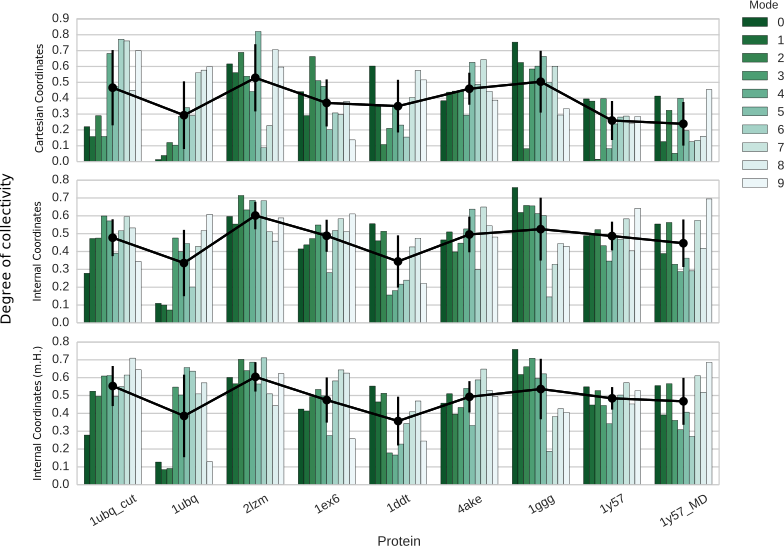
\includegraphics[width=\linewidth, height=\textheight, keepaspectratio]{cut_9_avg_coll}
\caption{Detailed study of the degree of collectivity per mode, structure and method. Cutoff has been set to 9 \angstrom. The Hessian modification method (m.H.) produces only slight improvements, generally concentrated in higher frequency modes.}
\label{fig:cut_9_avg_coll}
\end{figure}

The detailed view of mode collectivities for a cutoff of 9 \angstrom  is shown in Fig. \ref{fig:cut_9_avg_coll}. We can see how the collectivity of IC modes is higher, especially that of the lower frequency modes. The differences between 1ubq\_cut and 1ubq are of particular interest. In these two cases, the collectivity values of the lower frequency modes of 1ubq are pretty small for all three methods, and they increase perceptibly in 1ubq\_cut. This must be caused by the only difference between these two structures: the appearance of the C-terminal loop. The structure with the loop (1ubq) is severely suffering from the ``tip effect'' due to the flexibility of the final loop, perfectly illustrating how this effect can worsen the collectivity of the modes.  

From the analyses performed on this data set, we can conclude that IC modes have higher collectivity, and  that this collectivity is more robust to changes in the elastic network.  

\subsubsection{Comparison between the CC and IC mode spaces}

We also wonder to which extent the mode space spanned by the CC and IC modes is similar. To this end we will use two measures: the cumulative overlap and the root mean square inner product (RMSIP). Both of them are based on the mode overlap operation, which measures the projection of one mode over the other. It can be calculated as:
\begin{equation}
O_{ij} = \frac{\left | P_i . M_j \right |}{{\Arrowvert P_i\Arrowvert}{\Arrowvert M_j\Arrowvert}} .
\end{equation}
Its value ranges from 0 to 1, meaning 1 a perfect overlap.  

The Cumulative overlap \cite{yang_close_2008} measures to which extent a range of modes can capture the motion of a single mode. It is calculated as
\begin{equation}
CO_i(k)= (\sum_{j}^{k} O_{ij}^2)^\frac{1}{2},
\end{equation}
where $i$ is the mode we are checking and $[j,k]$ is the range of modes we will use to explain the first. Its value is, again, in the range from 0 to 1, meaning 1 a perfect match (assuming perfect orthogonality of the modes).   

Finally, the RMSIP \cite{amadei_convergence_1999,leo-macias_analysis_2005} measures how the normal mode space spanned by a range of modes overlaps with another range of modes. It is calculated as  
\begin{equation}
RMSIP(l,m) = \left( \frac{1}{l} \sum_{i=1}^l \sum_{j=1}^m {(P_i.M_j)}^2 \right )^\frac{1}{2} .
\end{equation}
Its value is independent of the mode order and ranges from 0 to 1, meaning 1 that both normal mode spaces are identical.

It is important to note that the modes coming from the IC conversion and PELE ANM model are defined for a different number of atoms (all heavy atoms in the first case, $C_\alpha$s in the second) and, therefore, they represent very different mode spaces. In order to make the comparisons possible, we need to calculate the ANM modes for all heavy atoms.

The cumulative overlaps shown in Figs. \ref{fig:avg_cum_overlap_per_cutoff} and \ref{fig:cut_9_cumulative_overlap} indicate that both mode spaces can explain each other successfully, being 1ubq, 1ubq\_cut and 1y57\_MD the only exceptions. In general, increasing the cutoff makes the differences between mode spaces more noticeable. The calculations performed with cutoff distance equal to 9 \angstrom (Fig. \ref{fig:cut_9_cumulative_overlap}), show that lower frequency modes are generally the ones that find a best correspondence with the modes of the other space.

\begin{figure}
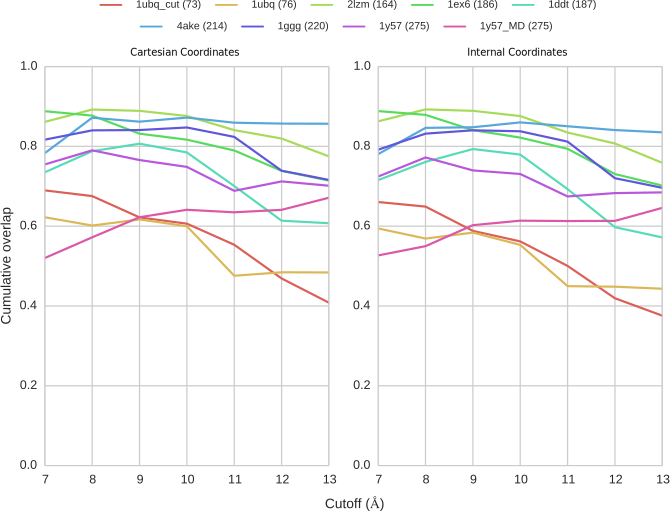
\includegraphics[width=\linewidth, height=\textheight, keepaspectratio]{avg_cum_overlap_per_cutoff}
\caption{ Average cumulative overlap for different cutoff distances, methods, and structures in our test set. Standard deviations are not shown for the sake of clarity.}
\label{fig:avg_cum_overlap_per_cutoff}
\end{figure}
 
\begin{figure}
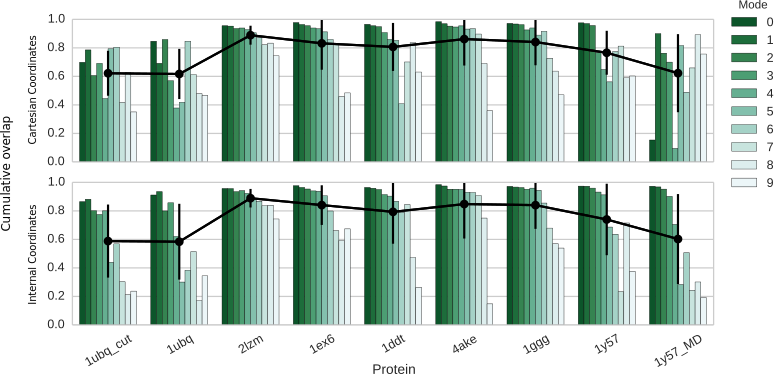
\includegraphics[width=\linewidth, height=\textheight, keepaspectratio]{cut_9_cumulative_overlap}
\caption{Detailed study of the cumulative overlap per mode, structure and method. Cutoff has been set to 9 \angstrom. In general, the rightmost modes (higher frequencies) are the ones with worst overlap.} 
\label{fig:cut_9_cumulative_overlap}
\end{figure}

Regarding the RMSIP for the modes calculated using a cutoff distance of 9 \angstrom, the mode space overlap is higher for the subspace of the low frequency modes, and decreases when more high frequency modes are added to the calculation (see Fig. \ref{fig:cut_9_rmsip_per_mode_range}), which correlates well with the observations made for Fig. \ref{fig:cut_9_cumulative_overlap}.

\begin{figure}
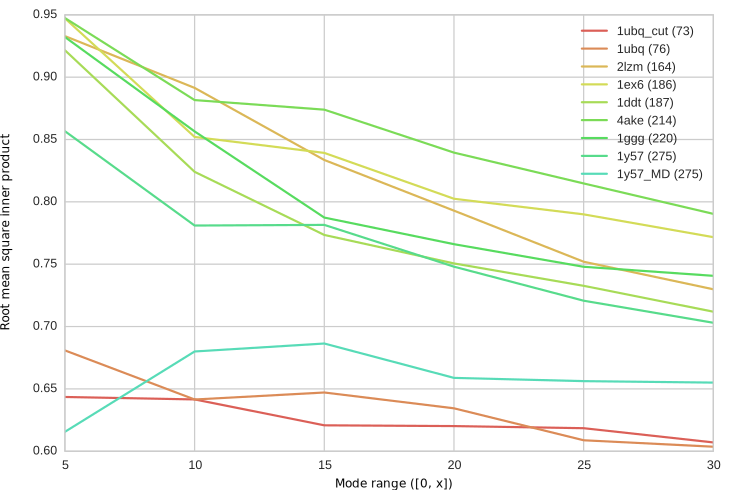
\includegraphics[width=\linewidth, height=\textheight, keepaspectratio]{cut_9_rmsip_per_mode_range}
\caption{RMSIP of CC and IC mode spaces. The x-axis shows the upper limit of the mode space tested (e.g, 10 means that the first ten modes are to be used to obtain the RMSIP). Both spaces look to be very similar, at least for the 5 lowest frequency modes. The similarities decrease as we move to modes of higher frequencies, with the only exceptions already commented in the cumulative overlap study.}
\label{fig:cut_9_rmsip_per_mode_range}
\end{figure}

\newpage
\cleardoublepage

\includepdf[pages=-]{pyrmsd.pdf}
\newpage
\cleardoublepage
\section[Supplementary materials: pyRMSD]{Supplementary materials for: pyRMSD: a Python package for efficient pairwise RMSD matrix calculation and
handling}

Comparing the performance of different algorithms is not straightforward. We can deduce some theoretical bounds,
but these might be too general to have any practical value, especially when comparing similar algorithms. When this
happens, the only way to go is to compare implementations.

In our implementations, good code design (especially reusability) had a bigger priority than optimality. All three
algorithm implementations have been coded sharing the same framework, reusing as many pieces of code as possible. This
enhances the comparability of our implementations, which may be suboptimal in the same degree, giving us a unique
opportunity of making a more fair performance comparison between them.

All benchmark tests were performed in BSC's Minotauro \cite{barcelona_supercomputing_center_minotauro_2015}, which has been built with Intel Xeon E5649 CPUs and NVIDIA M2090
GPUs. Only 1 GPU was reserved for CUDA runs. OpenMP runs used six threads at most.

\subsection{Algorithm performance comparison}
In order to get a good overview of each algorithm{}'s performance, we have checked the time that each of the three
algorithms need to complete the execution of each one of pyRMSD's basic methods (oneVsFollowing, pairwiseMatrix and
iterativeSuperposition). A 30k trajectory of Ubiquitin (reading only \calpha atoms) was used. The oneVsFollowing method has
been tested without and with input coordinates rotation, as this last adds overhead to QCP implementation due to the
mandatory rotation matrix calculation (QCP does not need to calculate it otherwise).

For basic linear operations (see Fig.~\ref{fig:pyrmsd_supp:1}), QCP has the best performance of all three, even when the rotation matrix is
calculated (oneVsFollowing(r) and iterativeSuperposition). The use of OpenMP smooths differences so much that choosing
one algorithm over the other becomes a mere matter of preference (see Fig.~\ref{fig:pyrmsd_supp:2}).

\begin{figure}
\includegraphics[width=\linewidth,height=\textheight,keepaspectratio]{pyrmsd_supp_serial_method_perf_comp.pdf}
\caption{ Comparison of the execution of three methods for the three available algorithm
implementations (serial).}
\label{fig:pyrmsd_supp:1}
\end{figure}

\begin{figure}
\includegraphics[width=\linewidth,height=\textheight,keepaspectratio]{pyrmsd_supp_openmp_method_perf_comp.pdf}
\caption{ Comparison of the execution of three methods for the three available algorithm
implementations (OpenMP).}
\label{fig:pyrmsd_supp:2}
\end{figure}

However, things change when comparing the performance of the pairwise matrix generation (see Fig.~\ref{fig:pyrmsd_supp:3}). Small performance
differences get amplified because of the quadratic nature of the problem. In this case, we observe that QCP excels by
achieving a 2x/4x speedup with respect to the other two, in both serial and OpenMP modes.

\begin{figure}
\includegraphics[width=\linewidth,height=\textheight,keepaspectratio]{pyrmsd_supp_matrix_gen_comp.pdf}
\caption{ Calculation time of a pairwise matrix from a 30k frames trajectory.} 
\label{fig:pyrmsd_supp:3}
\end{figure}

\subsection{QCP performance}
We want to compare all four implementations of QCP algorithm: serial, OpenMP, CUDA and CUDA with full matrix memory
allocation into the device. To this end, we will use the pairwiseMatrix method over Ubiquitin trajectories of 5, 10, 15,
20, 25, 30 and 35k frames.

We can see in the resulting plot (Fig.~\ref{fig:pyrmsd_supp:4}) that OpenMP version is about 5x faster than the serial one, and CUDA version
is about 8,5x faster.

\begin{figure}
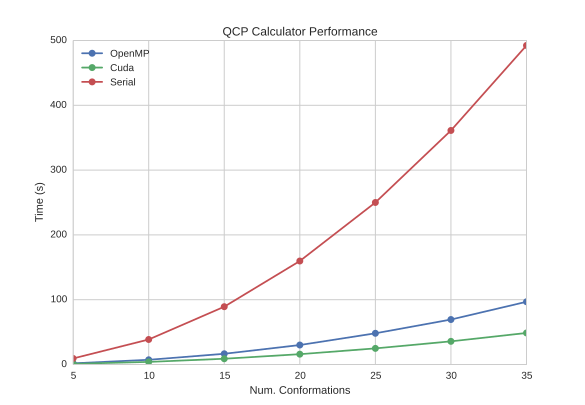
\includegraphics[width=\linewidth,height=\textheight,keepaspectratio]{pyrmsd_supp_qcp_perform_1.pdf}
\caption{ Performance comparison of serial, OpenMP and CUDA (single-precision) implementations of the QCP algorithm.}
\label{fig:pyrmsd_supp:4}
\end{figure}

After profiling the CUDA version, we saw that a considerable part of the time was spent in memory transactions from the
device to the host. The RMSD matrix is calculated line by line and, after each one of this calculations, the host
matrix representation is updated. This method can be successfully used in a broad range of GPUs, as it does not require
cards with big amounts of RAM. We implemented another method that holds the entire matrix in GPU's RAM. The speedup is
greater (11x compared with serial code), as memory transactions are performed only once (Fig.~\ref{fig:pyrmsd_supp:5}).

\begin{figure}
\includegraphics[width=\linewidth,height=\textheight,keepaspectratio]{pyrmsd_supp_qcp_perform_2.pdf}
\caption{ Performance comparison of CUDA implementations. 'Mem' versions hold the entire
matrix into memory, (s) versions use single-precision arrays and (d) versions use double-precision arrays.}
\label{fig:pyrmsd_supp:5}
\end{figure}

Finally, there are two things worth mentioning. The first one is that our CUDA implementation can be further improved by
enhancing work balance and memory coalescence. The second is that the use of single point precision in our QCP CUDA
implementation, contrary to what is expected, does not perform substantially better than the double precision
implementation. The reason for this behavior is again the big effort put into generalizing the code. pyRMSD uses
internally double-precision arrays to store coordinates and RMSD values. This implies that, when using GPUs without
double-precision support, a single-precision temporary buffer is to be filled at every host to device memory move.

\subsection{Input size response of \ QCP implementation}
The last benchmark established a clear relationship between the size of a trajectory (in frames) and the time needed to
do calculations. In this benchmark we want to fix the number of frames and test the impact of biomolecule sizes in
performance. The number of frames of the trajectory will be 10k, and the number of atoms of each one of the conformers
will be artificially increased at every step in order to calculate the pairwise RMSD matrix.

Both CUDA and OpenMP implementations, show a linear increase of the time needed to calculate the matrix (Fig.~\ref{fig:pyrmsd_supp:6}).
Incrementing conformer size does not increase or decrease performance.

\begin{figure}
\includegraphics[width=\linewidth,height=\textheight,keepaspectratio]{pyrmsd_supp_input_size_check.pdf}
\caption{ Input size response of the OpenMP and CUDA versions of the QCP algorithm.}
\label{fig:pyrmsd_supp:6}
\end{figure}

\subsection{Accuracy check}
While KABSCH algorithm tries to find an optimal rotation matrix, QTRFIT and QCP will use quaternions in order to get
this rotation. Does the base method affect accuracy? In this test, we have applied the oneVsFollowing method over the
first frame of a 10k frames Ubiquitin trajectory. Then we have calculated the root mean square of the differences,
which will be our index of RMSD value variation. 

In Table \ref{tab:pyrmsd_supp:rmsd_accuracy}, we can see that all implementations have an RMS different than 0, which means that all algorithms have
calculated different RMSD values. Kabsch's algorithm and QTRFIT have close results in spite of their different
approaches to calculating the superposition. QCP CUDA single-precision floating point version differs the most, being the
double-precision version the most accurate of both.

\begin{table}
\centering
\begin{tabular}{ c c c c c c } 

\toprule
Method & KABSCH & QTRFIT & QCP & \specialcell{QCP CUDA\\(Single)} & \specialcell{QCP CUDA\\(Double)}\\
\midrule

KABSCH & ~ & 2.308e-12 & 2.678e-12 & 1.028e-03 & 2.689e-12\\
QTRFIT & ~ & ~ & 1.568e-12 & 1.028e-03 & 1.547e-12 \\
QCP & ~ & ~ & ~ & 1.028e-03 & 8.926e-13\\
\bottomrule

\end{tabular}
\caption{Root Mean Square of the RMSD array differences for each of the algorithms.}
\label{tab:pyrmsd_supp:rmsd_accuracy}
\end{table}

It is important to note that, although QCP solves the problems of prior methods like Diamond's \cite{diamond_note_1988} algorithm instability in
rotations close to 180�, it can suffer from convergence problems derived from the use of Newton-Raphson root-finding
method.

However, differences are generally small, and RMSD is often used qualitatively, which means that, unless we require high
precisions, all algorithm implementations are interchangeable.

\subsection{OpenMP scalability}
We want to study the scalability of the OpenMP version of each of the algorithms. To achieve it we have calculated the
pairwise RMSD matrix of a 30k frames trajectory of Ubiquitin, using a different number of threads for each execution
(from 1 to 6).

It is not difficult to see that we obtain a linear speedup, with a maximum of 5.6-5.8x for six threads (compared with the
one thread run), which is close to the theoretical maximum speedup (6x for six threads) (Fig.~\ref{fig:pyrmsd_supp:7}, \ref{fig:pyrmsd_supp:8}).

\begin{figure}
\includegraphics[width=\linewidth,height=\textheight,keepaspectratio]{pyrmsd_supp_omp_scalability.pdf}
\caption{ Time needed to compute a pairwise matrix from a 30k frames trajectory using a
different number of threads.}
\label{fig:pyrmsd_supp:7}
\end{figure}

\begin{figure}
\includegraphics[width=\linewidth,height=\textheight,keepaspectratio]{pyrmsd_supp_speedup_per_thread.pdf}
\caption{ Percentage of speedup per thread added to the calculation. Speedup is almost
linear with number of threads.}
\label{fig:pyrmsd_supp:8}
\end{figure}

\subsection{Comparison with existing packages}
As a final test, we will compare pyRMSD with other software packages that include RMSD calculation features. We have
chosen four publicly available open source packages:

\begin{description}
	\item [g\_rms]  Is a C-written command line program part of the Gromacs \cite{berendsen_gromacs_1995} suite. Its main feature is the fast creation of
	distance matrices from trajectories.
	\item [Prody \cite{bakan_prody_2011-2}] A Python package which offers very interesting features to load and analyze biomolecule trajectories,
	including a complete PDB parser and a powerful selection language.
	\item [Biopython \cite{cock_biopython_2009-1}] A mature Python package which offers numerous bioinformatic computational tools.
	\item [PyVib2 \cite{fedorovsky_pyvib2_2007}] A pure Python package used to analyze vibrational motion and spectra of molecules.
\end{description}

Our comparison will be based on two measures: calculation time and integration complexity. To this aim we have created 4
scripts \footnote{The scripts can be found in \url{https://github.com/victor-gil-sepulveda/pyRMSD-Comparison.git}}. 
Every script calculates the RMSD
matrix of a trajectory twice, first using one of the aforementioned packages, and then replicating the same calculation
using pyRMSD (serial). Integration complexity has been measured as the ratio between the number of effective code lines
necessary to program the task with the tested package and pyRMSD. Performance has been calculated as the ratio of the time
needed to complete the task by the tested package over the time required by pyRMSD. All tests were performed on a workstation 
with an Intel Xeon W3530 CPU (four cores at 2.80GHz) with 12GB of RAM. 

\begin{sidewaystable}
\caption{Comparison of the time, lines of code, speedup and integration complexity (I.C.) needed to complete an RMSD collective operation.}
\centering
\begin{center}
\begin{tabular}{ r r c c c c c c }
\toprule
Method & Frames & Time (s) & Time pyRMSD(s)& 
 Lines of code & Lines of code (pyRMSD) & Speedup & I. C. \\ 
\midrule

\textbf{g\_rms} & 10 & 0.0564 & 0.0466 & 24 & 3 & 1.21 & 8 \\ 
~ & 100 & 0.7421 & 0.488 & ~ & ~ & 1.52 & ~ \\ 
~ & 1000 & 62.5245 & 14.6778 & ~ & ~ & 4.26 & ~ \\ 
\textbf{Prody} & 10 & 0.1698 & 0.0008 & 6 & 1 & 212.25 & 6 \\ 
~ & 100 & 3.408 & 0.0587 & ~ & ~ & 58.06 & ~ \\ 
~ & 1000 & 312.7806 & 6.0187 & ~ & ~ & 51.97 & ~ \\ 
\textbf{PyVib2} & 10 & 4.069 & 0.0001 & 7 & 1 & 40690.00 & 7 \\ 
~ & 100 & 450.1247 & 0.0995 & ~ & ~ & 4523.87 & ~ \\
~ & 1000 & 30332.6163 & 10.372 & ~ & ~ & 2924.47 & ~ \\ 
\textbf{Biopython} & 10 & 2.012 & 0.0008 & 8 & 1 & 2515.00 & 8 \\ 
~ & 100 & 219.6425 & 0.0572 & ~ & ~ & 3839.90 & ~ \\ 
~ & 1000 & 22003.5187 & 6.0966 & ~ & ~ & 3609.15 & ~ \\ 

\bottomrule
\end{tabular}
\end{center}
\label{tab:pyrmsd_supp:speedup}
\end{sidewaystable}

Table \ref{tab:pyrmsd_supp:speedup} shows that pyRMSD is always faster than the other packages. In the last three cases, this is because
that RMSD calculations are also written in pure python (which includes the use of numpy), while in pyRMSD these have
been written as C extensions. These packages have not been specifically designed to handle RMSD collective operations,
which explains why more lines of code are needed. Biopython and PyVib2 RMSD-related features are indeed constrained to
the pairwise RMSD case, while Prody can calculate rows of the matrix using only one function. This makes the last
faster and easier to use in this scenario. g\_rms is considerably faster than the others, as it has been written in C
and because of its narrower scope. However, to use it within a Python script, the user will need to create a wrapper to
control the program execution (here simplified by the utilization of the `expect' command), and a method to parse program
results. This adds extra complexity to the code as well as a performance penalty.







\newpage
\cleardoublepage

\includepdf[pages=-]{pyproct.pdf}
\newpage
\cleardoublepage
\section[Supplementary materials: pyProCT]{Supplementary materials for: pyProCT: Automated Cluster Analysis for Structural Bioinformatics}
\subsection{Implemented clustering algorithms}

In this section, we will review the algorithms currently implemented
in pyProCT. For each of these, we will briefly describe how it works,
how its parameters are generated (if automatic generation is triggered)
and the structure of each parameter objects, so that users can define
them inside the script.


\subsubsection[DBSCAN]{DBSCAN \cite{ester_density-based_1996}}

DBSCAN\footnote{Density-Based Spatial Clustering of Applications with Noise} 
is a density-based clustering algorithm. Density is given by the use
of 2 parameters: `eps', that defines a distance radius centered on
one element, and `minpts', that specifies the minimum number of neighboring
points for that element to be considered part of a cluster. 

The algorithm classifies elements into three categories: not classified,
noise and core elements. All elements are initially set to `not classified'.
The `core' elements are those that have at least `minpts' elements
in an `eps' radius and also the elements inside the `eps' radius of
a `core' element (which will be border points). All not `core' elements
are classified as 'noise' and will not be part of the clustering. 

One of the key issues of DBSCAN is the proper selection of its 'eps'
and `minpts' parameters. High density combinations can produce very
noisy clusterings (which, depending on the context can be an issue
or a feature), and low density combinations can easily lead to the
singleton clustering (a clustering with only one cluster encompassing
all elements). Because of its dependency on the element density, it
can have problems detecting clusters if there are different density
regions in the dataset.


\subsubsubsection{Parameters generation strategy} 

The implemented parameters generator is based on the details given
in the original articles \cite{ester_density-based_1996, sander_density-based_1998-2}
as well as the method of Ankerst 	extit{et al.} \cite{ankerst_optics_1999-1}.
Briefly: 

\begin{enumerate}
\item pyProCT will recreate k-distance lists for some k values ( 
$ k < \log \left ( \abs{D} \right )$ 
as indicated in the literature). 

\item For each of the k-distance lists, an `eps' value will be chosen so
that the generated noise falls between 0\% and the maximum allowed
noise (plus a 2.5\% margin). The value of k in that k-distance list
will be used as the value of `minpts' in that parameter pair. 
\end{enumerate}

In addition, we add the parameter choice suggested by Zhou 	extit{et al.}\cite{zhou_research_2012-1}.


\subsubsubsection{Parameters object structure }
\begin{lstlisting}[language=json,firstnumber=1] 
{ 	
	"eps": Real,
	"minpts": Integer 
}
\end{lstlisting}


\subsubsection{GROMOS}

First found in the work of Daura 	extit{et al.} \cite{daura_peptide_1999,daura_folding-unfolding_1999-1},
it is also a density-based algorithm. As it looks that the algorithm
has no name, we named it after the flag that the g\_cluster tool\cite{berendsen_gromacs_1995}
receives to use it. With a simpler behaviour than DBSCAN, it was thought
to adapt to the ideal expected characteristics of datasets coming
from the conformational search of small peptides (well-separated regions
centered in metastable states). 

The algorithm repeats a loop that ends when all elements have been
clustered:

\begin{algorithm}[H]
\caption{GROMOS algorithm}
\begin{algorithmic}[1]
\Input $D$, the data set
\Input $cutoff$, the cutoff radius
\Output $C$, a set of clusters
\State $D_{tmp} \gets D$ \;
\While{ $D_{tmp} \neq \emptyset$}
\State $e \gets$ mostDense($D_{tmp}$)\;
\State $neig \gets$ neighbours($e$,$cutoff$)\;
\State $c \gets \{e, neig\}$\;
\State addCluster($c$, $C$)\;
\State $D_{tmp} \gets D_{tmp} \setminus c$\;
\EndWhile
\State \textbf{return} C
\end{algorithmic}
\end{algorithm}

\begin{description}
\item [mostDense()] Find the element with more neighbors inside the given cutoff radius
(to find the densest zone). 
\end{description}

\subsubsubsection{Parameters generation strategy}

The goal here is to find a finite range of cutoffs, exactly as it is done with
the `k' parameter in k-medoids or `num\_clusters' in the random grouping
algorithm. The minimum value for the cutoff parameter is 0, generating
a trivial clustering in this case (a clustering where each element
is a cluster). In order to get an estimation of the maximum value,
we choose the 3 most separated elements of the dataset. We can ensure
that the second longest side of the triangle with this 3 elements
as vertices will be the minimum radius that encompasses all elements
of the dataset, producing a singleton clustering, and thus it is the
upper limit of the cutoff range. Once the maximum and minimum are
known, we can obtain equidistant values for the cutoff within this
range.


\subsubsubsection{Parameters object structure}
\begin{lstlisting}[language=json,firstnumber=1] 
{ 	
	"cutoff": Real
}
\end{lstlisting}


\subsubsection{Hierarchical clustering}

pyProCT uses an external package \cite{mullner_fastcluster_2013}
that implements an agglomerative hierarchical clustering algorithm.
Agglomerative hierarchical algorithms start with all elements of the
dataset forming single clusters (a trivial clustering) and every step
it merges the closest clusters by means of a proximity function (only
`single linkage' and `complete linkage' options can be used). The
agglomerative step represents the dataset as a tree (dendrogram) that
has to be cut in order to retrieve the clustering. The distance at
which the cut is performed is called the cutoff distance.


\subsubsubsection{Parameters generation strategy}

Getting the dendogram cut is computationally cheap compared to the
hierarchical matrix calculation. In this case, pyProCT will generate
clusterings until it finds the range of cutoffs in which the resulting
clustering falls within the range of allowed number of clusters. This
range will be refined in order to get more clustering candidates.


\subsubsubsection{Parameters object structure}
\begin{lstlisting}[language=json, firstnumber=1] 
{ 	
	"cutoff": Real, 
	"method": String in ["single", 
			   "complete"] 
}
\end{lstlisting}
\begin{description}
\item [method] If its value is `single', the single linkage method
is used to calculate the proximity of clusters. This proximity is
then defined as the minimum distance between any two points in that
clusters. If `complete' is used instead, the proximity of two clusters
is measured as the maximum distance between any two elements of different
clusters. Various combinations of method-cutoff are possible in
the parameters list, but due to performance reasons, only the `method'
value of the first parameter object in the list will be used.
\end{description}

\subsubsection{K-Medoids}

Is a partitional algorithm similar in concept to k-means. Because
of its beautiful simplicity, our implementation is based on Lloyd's
k-means algorithm \cite{lloyd_least_1982} instead that on other k-medoids
specific algorithms (like PAM \cite{kaufman_finding_1990-1}).Roughly the algorithm works as follows:

\begin{algorithm}[H]
\caption{K-Medoids algorithm}
\begin{algorithmic}[1]
\Input $k$, number of clusters
\Output $C$, a set of clusters
\State medoids $\gets$ initialSeeding(k)\;
\While{$\neg$ convergence() $~\land \neg$ maxStepsReached()}%
\State C $\gets$ labelElements()\;
\State medoids $\gets$ calculateMedoids(k)\;
\EndWhile
\State \textbf{return} C
\end{algorithmic}	
\end{algorithm}

\begin{description}
	\item[convergence()]  Checks if how the labeling of current iteration has changed with respect to the last iteration.
	\item[labelElements()] Labels each element of the dataset with the cluster of its closer medoid. 
\end{description}

K-Means-like algorithms will perform better detecting convex clusters.

\subsubsubsection{Parameters generation strategy}

A globally-defined or used-defined maximum number of parameter sets
(`max') will be generated. Each of the parameter sets will have its
`method' field set to `EQUIDISTANT' and its `k' field will is calculated as 
$(min\_clusters+step \times n$ where $0<=n<=max$ and $step$ is $\nicefrac{(max\_clusters-min\_clusters)}{max}$.

\subsubsubsection{Parameters object structure}
\begin{lstlisting}[language=json,firstnumber=1] 
{ 	
	"k": Integer, 	
	"seeding_type": String in ["RANDOM", 
			      "EQUIDISTANT", 
			           "GROMOS"], 	
	"seeding_max_cutoff": Real 
}
\end{lstlisting}

\begin{description}
	\item [k] Number of clusters to be created. 
	\item [seeding\_type] Method used for initial medoid seeding. 
	\item [seeding\_max\_cutoff] Only used when `seeding\_type' =
	GROMOS. Maximum cutoff radius for the GROMOS algorithm to generate
	the initial medoids.
\end{description}

The algorithm is very sensitive to the initial seeding configuration
(the initial placement of the medoids). Three seeding methods are
provided: 

\begin{description}
	\item [RANDOM] Uses a random choice of elements from the dataset
	as initial medoids. If used, the parameter will be replicated `tries'
	times (default: 10) with different random seeds. 
	\item [EQUIDISTANT] Divides the dataset in k consecutive parts
	and uses their central element as medoid. Useful if we suspect that
	sequence order and geometrical likeness are correlated (like in MD
	sequences). 
	\item [GROMOS] It will execute GROMOS algorithm with decreasing
	cutoffs until `k' or more clusters are generated. Initial medoids
	will be the centers of this clusters. It is specially useful if clusters
	were well separated. 
\end{description}


\subsubsection{Spectral Clustering}

This algorithm uses the spectral properties of the dataset (viewed
as a graph). It is said that it can achieve better results than k-means
or hierarchical clustering algorithms.

The implemented version of the algorithm is described in the detailed
review written by Ulrike von Luxburg \cite{luxburg_tutorial_2007},
based on the Normalized Spectral Clustering\cite{shi_normalized_2000}).
It needs to perform six steps:

\begin{algorithm}[H]
\caption{Spectral clustering algorithm}
	\begin{algorithmic}[1]
		\Input {$M$, a distance matrix}
		\Input {$D$, initial data set}
		\Input {$k$, number of clusters}
		\Output $C$, a set of clusters
		\State $A \gets$ adjacencyMatrix($M$)\;
		\State $Deg \gets$ degree($A$)\;
		\State $L \gets$ laplacian($A$, $Deg$)\;
		\State $eigvec \gets$ caclEigenvectors($L$,$k$)\;
		\State $C_e \gets$ kMedoids($eigvec$, $k$)\;
		\State $C \gets$ map($C_e$, D)\;
		\State \textbf{return} C
	\end{algorithmic}
\end{algorithm}

\begin{description}
	\item [adjacencyMatrix()] Constructs a similarity graph by applying a kernel to the distance matrix. 
	\item [degree()] Computes the degree matrix and adjacency matrix. 
	\item [laplacian()] Computes the (unnormalized) Laplacian. 
	\item [caclEigenvectors()] Computes the first $k$ generalized eigenvectors. 
	\item [kMedoids()] Clusters the eigenvector matrix as if each row was a point. 
	\item [map()] Maps each of the eigenvectors to the elements of the dataset (row $i$ corresponds to element $i$).
\end{description}

\subsubsubsection{Parameters generation strategy}

The sigma global parameter, used to calculate the adjacency matrix,
can be set by the user. If not, pyProCT will use a local sigma calculation
strategy \cite{zelnik-manor_self-tuning_2004-1} to build it. `k' parameter
is generated using the same approach than in the k-medoids case.


\subsubsubsection{Parameters object structure}
\begin{lstlisting}[language=json,firstnumber=1] 
{ 
	"k": Integer, 
	"use_k_medoids": Boolean 
}
\end{lstlisting}

\begin{description}
\item [use\_k\_medoids] \hfill \\If set to true, the k-medoids algorithm will
be used to cluster eigenvalues. If set to false, k-means will be used
instead.
\end{description}

\subsubsection{Random Grouping}

This algorithm assigns random cluster labels to the different elements
in the dataset. It cannot be considered a real clustering algorithm,
but it is useful to compare the behaviour of certain ICVs with more
sphisticated algorithms. It has been implemented in two ways: 

\begin{description}
\item [FakeDistributionRandomClusteringAlgorithm] \hfill \\Generates clusters
with certain per cluster population distribution (e.g. First cluster
70\% of the elements, second 20\%, third 5\% and so on) 
\item [RandomClusteringAlgorithm] \hfill \\Generates a totally random clustering
(random number of clusters and random cluster assignment) or a random
clustering with a predefined number of clusters.
\end{description}

\subsubsection{Parameters generation strategy}

The same strategy used in k-means to calculate the k value will be used 
here for num\_clusters.

\subsubsection{Parameters object structure}

Only RandomClusteringAlgorithm is accessible through the script, and
it only needs one parameter: 

\begin{lstlisting}[language=json,firstnumber=1] 
{ 
	"num_clusters": List(Integer)
} 
\end{lstlisting}

\begin{description}
\item [num\_clusters] \hfill \\Number of clusters to be created (analogue
to `k' in other algorithms).
\end{description}



\subsection{Clustering properties and quality functions}
\label{sec:pyproct_supp_2}

pyProCT implements functions which goal is to retrieve information
from the generated clusterings to evaluate them. Some of these functions
retrieve properties from the clustering (\textquotedblleft properties\textquotedblright ),
other functions evaluate the quality and form the objective part of the
clustering hypothesis. In this section we will define and formalize
both of them.


\subsubsection{General definitions}

\begin{enumerate}
\item $D$ is a set containing all the elements of the dataset with $\abs D$
number of elements (number of datum in the dataset e.g. conformations,
distances, etc). 
\item $C=\{C_{1},C_{2},\dotsc C_{k}\}$ is a clustering of $k$ clusters,
where $\abs C$ is its number of clusters ( $\abs C=k$ in this case)
and $|C_{i}|$ is the number of elements of cluster $i$. Also:
\begin{equation}
\forall C_{i},C_{j}\in C,\quad i\neq j\quad C_{i}\cap C_{j}\equiv\emptyset
\end{equation}

\item $D_{C}\subseteq D$ is the set of clustered elements, which can differ
from the initial set if some elements were considered as noise and
thus discarded.
\begin{eqnarray}
D_{C} & \equiv & \bigcup_{i=1}^{k}C_{i},
\end{eqnarray}

\item $d(a,b)$ is a distance metric (dissimilarity function) applied to
an element $a\in D$ and an element $b\in D$.
\item $m_{i}$ is the medoid of cluster $C_{i}$ so that:
\begin{equation}
m_{i}\in C_{i}
\end{equation}
\begin{equation}
\forall a,b\neq m_{i}\quad a,b\in C_{i}\quad d(a,b)\geq d(a,m)\wedge d(a,b)\geq d(b,m)
\end{equation}

\item As stated before singleton clustering is a clustering with one cluster
that holds all the elements of the dataset. In a trivial clustering,
each element of the dataset forms its own clustering.
\begin{equation}
\abs C_{singleton}=1
\end{equation}
\begin{equation}
\abs C_{trivial}=\abs{D_{C}}
\end{equation}

\end{enumerate}

\subsubsection{Properties}

The properties are functions that allow users to query about simple
traits and statistics of the clustering. The information returned
by this functions is purely descriptive and, in general, not usable
for evaluation purposes. Eight properties have been defined:

\begin{description}
\item [{Details~(String)}] Returns a string containing information about
the type of clustering algorithm and the parameters used to generate
it. 
\item [{NumClusters~(Integer)}] Returns the number of clusters ($\abs C$). 
\item [{MeanClusterSize~(Real)}] Mean number of elements per cluster:

\begin{equation}
mcs(C)=\frac{\sum_{i=1}^{k}|C_{i}|}{\abs C}
\end{equation}

\item [{NumClusteredElems~(Integer)}] Returns the number of elements that
were clustered. It can be lower than the initial number of elements
if noise was eliminated. Is defined as:
\begin{equation}
nce(C)=\sum_{i=0}^{|C|}|C_{i}|\equiv|D_{C}|
\end{equation}

\item [{NoiseLevel~(Real)}] Calculates the ratio of clustered elements
over the number of initial elements:
\begin{equation}
nl(C,D)=\frac{\sum_{i=1}^{k}|C_{i}|}{\abs D}\equiv\frac{|D_{C}|}{|D|}
\end{equation}

\item [{ClustersTo90~(Real)}] Returns the minimum number of clusters needed
to accumulate 90\% of the clustered elements. 
\item [{PercentInTop~(Real)}] Calculates the percentage of clustered elements
owned by the biggest cluster. 
\item [{PercentInTop4~(Real)}] Calculates the percentage of clustered
elements owned by the four larger clusters.
\end{description}

\subsubsection{Quality functions }

Sometimes referred to as Clustering Validity Indices (CVI), are functions
which aim is to tell at which degree clusterings are an artificial
partition or reflect the real inner structure of the dataset (assuming
that it exists). Quality functions must use only internal information
of the clustering, that is, not to be based on a solution that is
considered correct.

The following are some initial definitions that will help us to characterize
them:
\crparagraph{Within cluster distance} The sum of all distances inside a cluster.

\begin{equation}
wd(C_{i})=\sum_{a,b\in C_{i}}d(a,b)
\end{equation}

\crparagraph{Between cluster distance} Sum of the pairwise distances between elements
belonging to two different clusters.
\begin{equation}
bd(C_{i},C_{j})=\sum_{a\in C_{i}}\sum_{b\in C_{j}}d(a,b)
\end{equation}

\crparagraph{Average~distance} Average of all pairwise distances between the elements
inside a cluster.

\begin{equation}
avg(C_{i})=\frac{wd(C_{i})}{|C_{i}|}
\end{equation}

\crparagraph{Standard~deviation~of~distance} The standard deviation of all
pairwise distances of the elements inside a cluster.

\begin{equation}
stdev(C_{i})=\sqrt{\frac{\text{1}}{|C_{i}|}\sum_{a\in C_{i}}d^{2}(a,m_{i})}
\end{equation}

\subsubsubsection[Cohesion]{Cohesion \cite{michael_introduction_????}}

Is a measure of cluster compactness. The cohesion factor measures
the inner similarity of a cluster. Its value for one cluster is calculated
by summing up the distance of all elements belonging to that cluster.
Its value for a clustering can be defined as the sum of its clusters
partial cohesions weighted by the inverse of the cluster size. Due
to the use of dissimilarity metrics, the interpretation of cohesion
can be misleading: the smaller its value, the more compact the clusters
are.

\begin{equation}
Ch(C)=\sum_{C_{i}\in C}\frac{\text{1}}{C_{i}}wd(C_{i})
\end{equation}


A cohesion value of 0 can be obtained with the singleton clustering.
It reaches its maximum value in a trivial clustering ($|D_{C}|^{-1}wd(D_{C})$).

Te actual implementation in pyProCT is a more intuitive redefinition of Cohesion, as 
an increment of cluster compactness will also increase this index value:

\begin{equation}
Ch(C)=1-\frac{Ch(C)}{|D_{C}|^{-1}wd(D_{C})}
\end{equation}

Its value ranges between 0 and 1.


\subsubsubsection[Separation]{Separation \cite{michael_introduction_????}}

Measures how distinct a cluster is from other clusters (how isolated
a cluster is from the others). In practice, it calculates the sum
of distances weighted by its cohesion:

\begin{equation} Sep(C)=\sum_{\substack{i=1\\ j>i}}^{k} \frac{bd(C_i,C_j)}{Ch(C_i)} \end{equation}

When its value increases, cluster separation increases. Its value
ranges from 0 (trivial clustering) to infinity (singleton clustering,
which implies $Ch(C_{i})\equiv0$.

\subsubsubsection[Compactness]{Compactness \cite{he_quantitative_2004-1}}

Compares the standard deviation (std. dev.) of the clustered dataset
(std. dev. of its clusters) with the std. dev. of the whole dataset.
Note that the std. dev. calculation function is defined using the
medoid of the cluster instead of the mean point.

\begin{equation}
Cmp(C)=\frac{1}{\abs C}\sum_{i=1}^{|C|}\frac{stdev(C_{i})}{stdev(D_{C})}
\end{equation}


Maximizing its value minimizes compactness.


\subsubsubsection[Gaussian Separation]{Gaussian Separation \cite{he_quantitative_2004-1}}

Is a prototype-based separation index where distances are attenuated
using an exponential. This intends to produce the same behaviour that
some exponential kernels used to calculate the adjacency matrix in
graph-like representations of the dataset: diminish long range distances
and sharpen subgraphs contours.

\begin{equation} 
Gsep=\frac{1}{\abs C(\abs C-1)}\sum_{\substack{i,j = 1,\dotsc,\abs C \\ j \neq i}} e^{\frac{-d^2(m_i,m_j)}{2\sigma^2}}
\end{equation} 

Maximizing its value maximizes separation.


\subsubsubsection[Davies-Bouldin]{Davies-Bouldin \cite{davies_cluster_1979}}

A prototype-based measure that compares compactness (represented by
the average of intra-cluster distances) and separation (distance between
the prototypes).

\begin{equation} 
Db(C)=\frac{1}{\abs C}\sum_{i=1}^{\abs C}max\substack{j \in 1,\dotsc,\abs C \\ j \neq i} \left(\frac{avg(C_i)+avg(C_j)}{d(m_i,m_j)}\right)
\end{equation} 

Measures compactness and separation. The smaller the value is, the better
overall quality the clustering has.


\subsubsubsection[Dunn]{Dunn \cite{dunn_fuzzy_1973-1,kryszczuk_estimation_2010-2}}

Ratio of the minimum inter-cluster distance and the maximum intra-cluster
distance.

\begin{equation}
mind(C_i)=min_{r,t\in C_i} d(r,t)
\end{equation}

\begin{equation}
maxd(C_i,C_j)=max_{\substack{ r \in C_i \\ t \in C_j}} d(r,t)
\end{equation}

\begin{equation}
Dunn(C)=\frac{min_{C_i \in C}(mind(C_i))}{max_{\substack{C_i,C_j \in C\\i \neq j}} (maxd(C_i,C_j))}
\end{equation}

Dunn index evaluates compactness and separation simultaneously. Quality
clusterings should have high values for this function.


\subsubsubsection[Calinski-Harabasz]{Calinski-Harabasz \cite{calinski_dendrite_1974-1}}

Another variation of the intra and inter-cluster distances ratio
calculation.

\begin{equation} 
A_k(C) = \frac{1}{|D_C|-\abs C}  \sum_{i=1}^{\abs C} (|C_i|-1)(avg(D_C)-avg(C_i)) 
\end{equation}

\begin{equation} 
CH(C)=\frac{avg(D_C)+\frac{|D_C|-\abs C}{\abs C -1}A_k}{|D_C|-A_k(C)} 
\end{equation}

It also measures compactness and separation.The higher the value is,
the better quality the clustering has.


\subsubsubsection[Silhouette]{Silhouette \cite{rousseeuw_silhouettes_1987-1}}

Useful when distances are on a ratio scale (for instance euclidean
distance), allowing to measure compactness and separation altogether
by calculating the pairwise difference of inter and intracluster distances.
The Silhouette index for a single element of a cluster can be calculated
as:

\begin{equation} 
S(e) = \left\{ \begin{array}{l l} \frac{b(e)-a(e)}{max(a(e),b(e))} & \quad \text{if $|C_i|>1$} \\
    0 & \quad \text{if $|C_i| \leq 1$} \end{array} \right.
\end{equation}

Where $a(e)$ is the average inner dissimilarity of its cluster and
$b(e)$ is the outer dissimilarity of this element with the other
clusters, calculated as follows:

\begin{equation} 
e \in C_e
\end{equation}

\begin{equation} 
a(e)=\sum_{\substack{t\in C_e\\t \neq e}}d(e,t)
\end{equation}

\begin{equation} 
b(e)=\sum_{\substack{\forall t\in C_i\\t \neq e \\ C_f \neq C_e}}d(e,t)
\end{equation}

Cluster and clustering values for this index can be calculated as
the cluster average and global average of their per-element values.
Its value ranges from -1 (worst quality) to 1 (best quality).


\subsubsubsection[PCAanalysis]{PCAanalysis \cite{amadei_essential_1993}}

Calculates the axes of variance and gives an estimation of the amount
of variance in each axis for each cluster. The final value of this
index will be the average value of the variance of the major variance
axis for each cluster. As with other compactness measures, it depends
on the size of the clusters. The higher the value is, the less compact
the clusters are. Measures compactness (by means of variance).


\subsubsection{Graph cut indices}

The distance relationships between elements of the clustering can
be viewed as a similarity graph were each vertex is an element and
edges are weighted by their distances. In general, small values for
this functions mean good quality of the partition (almost all are
a sum of adjacency weights). Clustering can then be seen as a
partitioning problem where one objective graph cut function is optimized.
First, we will need to define some helper functions. Note that,
in this case, the distances are the edge values, and are related to the 
adjacency matrix:

\subsubsubsection{Degree of a node}
Sum of the weights of the edges that contain this node.

\begin{equation}
deg(a)=\sum_{\forall i, b \in C_{i}} d(a,b)
\end{equation}

\subsubsubsection{Internal volume}
Is defined as the sum of all the weights of the edges of one partition, including those that connect with other partitions). As each edge must be counted only once and internal edges are counted twice, final  must be multiplied by 0.5. Can be seen as the sum of degrees too.

\begin{equation}
vol(C_{i})= \frac{1}{2} \sum_{n\in C_{i}} deg(n)
\end{equation}

\subsubsubsection{Cut}
Sum of the weights of the edges that have to be removed in order to separate two 
components of the graph. Its value is 0 if both subgraphs are not connected.

\begin{equation} 
cut(C_{i})=\frac{1}{2}\sum_{i \in C_{i} , j \in \overline{C_{i}}} d(i,j) 
\end{equation}

\subsubsubsection[Normalized Cut]{Ncut (Normalized Cut) \cite{shi_normalized_2000}}
It is mainly a separation measure. Some authors divide it by the number of clusters.

\begin{equation}
NCut(C)= \frac{\sum_{i=1}^{k}\frac{cut(C)}{vol(C_{i})}}{k}
\end{equation}


\subsubsubsection[MinMaxCut]{MinMaxCut \cite{ding_min-max_2001-1}}
It is mainly a separation measure.

\begin{equation}
MinMaxCut(C)=\frac{1}{2}\sum_{i=1}^{k}\frac{cut(C_{i})}{vol(C_{i})}
\end{equation}

\subsubsubsection[RatioCut]{RatioCut \cite{hagen_new_1992}}
It is mainly a separation measure.

\begin{equation}
RatioCut(C)=\sum_{i=1}^{k}\frac{cut(C_{i})}{|C_{i}|}
\end{equation}



\subsection{Input script}

pyProCT uses as input a human-readable JSON text file. Its file
extension can be arbitrarily chosen, however pyProCT will generally
produce this kind of files with a `.json' extension.

The input file describes how the software interacts with the underlying
hardware where it is being executed, how the clustering exploration
will be performed, and finally, which kind of post process operations
will be performed after the clustering has been obtained. This section
will be structured in 4 subsections, one for each of the main subsections
of the script (`global', `data', `clustering' and `postprocess').

Unless otherwise specified, each property or object will be represented
by a descriptor. This descriptor contains the label of the property
or JSON object (subsections), information about its data type, and
possible dependencies.

A label consists of a double colon separated list of the names of
the objects that encompass the property or subsection, followed by
its name. For instance, \textbf{x::y::z} corresponds to the JSON object:

\begin{lstlisting}[firstnumber=1,language=json,caption={Simple JSON object.}]
"x":{ 	
	"y":{
		"z":{}
	}
}
\end{lstlisting}

The nature of z will be specified after the label. Possible tags are: 

\begin{description}
	\item [{Subsection}] The item is another JSON object that can contain another
	subsections (JSON objects) and properties. 
	\item [{Integer}] The item is an integer value property. 
	\item [{Real}] The item is a real value property. 
	\item [{String}] The item is a string property. 
	\item [{List}] The item is an array of elements. 
\end{description}

If the value of the property has to be chosen from a limited list
of possible choices, this values will be enumerated in a ``value
in {[}choices{]}\textquotedblright{} clause. ``Optional\textquotedblright{}
will be added to the end of the descriptor if the property is optional.

Finally, if a property or subsection needs it, a dependency clause
will be added in front of the label. This dependency clause contains
the label it depends on and the value it needs to have, or, if it
just depends on its previous definition, an ``is defined\textquotedblright{}
clause.

Examples:

{[}\textbf{x::y::z} is defined{]} \textbf{x::y::t}

Means that x::y::t value will be ignored unless x::y::z has a value.

{[}\textbf{x::y::z} == ``m\textquotedblright {]} \textbf{x::y::t}

Means that x::y::t will not be used unless x::y::z is defined and
has value ``m\textquotedblright .

\begin{framed}
The rest of this section has been intentionally hidden as it no longer describes pyProCT input script. For 
updated information please visit the repository at \url{https://github.com/victor-gil-sepulveda/pyProCT}.
\end{framed}


\subsection{Results file}

The results file summarizes the whole clustering process and its results.
It contains extra information that can be processed afterwards with
the results viewer in order to gain more insight about the used quality
functions and criteria.


\subsubsection{Best clustering}

This section contains only one property that holds the identification string of the best
clustering.
\begin{lstlisting}[caption={Best clustering result ID},firstnumber=1,language=json]
{
	"best_clustering": String
}
\end{lstlisting}

\begin{description}
\item [best\_clustering] Id of the best clustering.
\end{description}

\subsubsection{Files}

This section stores a list of file objects, containing the details
of all generated files (included the results file itself):

\begin{lstlisting}[caption={The file details section of the results file},firstnumber=1,language=json]
{
	"files": List(FileDetailsObject)
}
\end{lstlisting}
A FileDetails object has the following structure:

\begin{lstlisting}[caption={FileDetails object},firstnumber=1,language=json]
{
	"path": String,
	"type": String in ['text','image'],
	"description": String
}
\end{lstlisting}

\begin{description}
\item [{path}] Complete path of the file
\item [{type}] `text' if the file is a human-readable txt file, or `image'
if it is a viewable image file.
\item [{description}] Contains a very brief description of the file contents.
\end{description}

\subsubsection{Trajectories}

A list containing objects with details of the trajectories used in
this clustering:

\begin{lstlisting}[caption={The trajectory details section of results file},firstnumber=1,language=json]
{
	"trajectories": List(TrajectoryDetailsObject)
}

\end{lstlisting}

Each TrajectoryDetails object has the following structure:

\begin{lstlisting}[caption={TrajectoryDetails object},firstnumber=1,language=json]
{
	"source": String,
	"conformations": Integer,
	"atoms": Integer
}
\end{lstlisting}

\begin{description}
\item [{source}] Complete path of this trajectory.
\item [{conformations}] Number of conformations (`model' sections) of
the pdb.
\item [{atoms}] Number of atoms of each conformation.
\end{description}

\subsubsection{Workspace}

Is a copy of the same section in the parameters file.

\subsubsection{Scores}

Contains the score value of each criterion for all non-filtered clusterings.

\begin{lstlisting}[caption={Possible score section for a clustering process that used two criteria and ended with two candidates},firstnumber=1,language=json] 
"scores": {
	"criterion_0": {
		"clustering_0001": 0.9822,
		"clustering_0002": 0.9935
	},
	"criterion_1": {
		"clustering_0001": 0.9150,
		"clustering_0002": 0.9229
	}
} 
\end{lstlisting}


\subsubsection{Timing}

Compiles the values of all timer objects in a list. These can be used
to rapidly assess the performance of the execution.

A timer object has the following structure:

\begin{lstlisting}[caption={Timer object},firstnumber=1,language=json]
{
	"name": String,
	"elapsed": Real
}
\end{lstlisting}

\begin{description}
	\item [{name}] Name of the step being checked.
	\item [{elapsed}] The duration of the step in seconds.
\end{description}

\subsubsection{Clustering information}

The clustering information section is indeed composed of 2 similar
sections: `selected' stores all non-filtered clusterings, and `not\_selected'
holds the ones that were filtered.

Both sections contain JSON objects with details of the generated clustering.
A clustering object is indexed by its id, and contains the following
subsections:

\textbf{clustering::clusters } List(ClusterObject)

A list of the clusters forming the clustering. See the input file
section \textbf{clustering\allowbreak::generation\allowbreak::clusters }for a description
of the format of a cluster object.

\textbf{clustering::total\_number\_of\_elements} Integer

The amount of clustered elements.

\textbf{clustering::number\_of\_clusters} Integer

The length of the clusters list.

\textbf{evaluation } Evaluation

An evaluation object containing the values of all calculated queries
and quality functions for this clustering.

\textbf{type} String in {[}`dbscan', `gromos', `hierarchical', `kmedoids',
`spectral', `random'{]}

Indicates which algorithm generated this clustering.

\textbf{parameters} ParametersObject

Parameters used by the algorithm to generate this clustering (as detailed
in the Algorithms section).

Clusterings under the `\_selected' key have slightly different
contents. They share all fields but the `evaluation' one, which changes
to `reasons'.

\textbf{reasons } List(ReasonObject)

Holds a list of reasons why the clustering was not considered for
evaluation. each reason object looks like this:

\begin{lstlisting}[caption={Reason object},
firstnumber=1, 
language=json, 
breakatwhitespace=true 
%,literate={\_}{}{0\discretionary{_}{\\}{}}
]
{
    "reason": String in ["TOO_FEW_CLUSTERS",
                        "TOO_MUCH_CLUSTERS", 
                           "TOO_MUCH_NOISE",
                "EQUAL_TO_OTHER_CLUSTERING"],
    "data": ReasonDataObject
}
\end{lstlisting}

\begin{description}
	\item [`reason'] The reason to exclude this clustering from the evaluation
	step. `TOO\_FEW\_CLUSTERS' and `TOO\_MUCH\_CLUSTERS' mean that the
	number of clusters is not into the allowed range. `TOO\_MUCH\_NOISE'
	means that the clustering had too much noise. `EQUAL\_TO\_OTHER\_CLUSTERING'
	means that an exact clustering has been already generated (with other
	algorithm or parameters).
	\item [`data'] Gives details about the reason to eliminate this clustering.
	For the first 3 cases, it will store the maximum/minimum value of the
	range and the current value for that clustering.
\end{description}

\begin{lstlisting}[caption={This clustering was not used because it had fewer clusters \(1\) than the minimum number of clusters allowed \(6\)},firstnumber=1,language=json]
{
	"reason": "TOO_FEW_CLUSTERS",
	"data": {
		"current": 1,
		"minimum": 6
	}
}
\end{lstlisting}

Data objects for `EQUAL\_TO\_OTHER\_CLUSTERING' reasons will only
store the id of the repeated clustering.

\begin{lstlisting}[caption={},firstnumber=1,language=json]
{
	"reason": "EQUAL_TO_OTHER_CLUSTERING",
	"data": {
		"id": "clustering_0003"
	}
}
\end{lstlisting}

\subsection{Clustering of a long trajectory (proof of concept)}
\label{sec:pyproct_supp_5}

In a cluster analysis, the function distance must be applied many
times to the different elements of the dataset. As pyProCT needs to
generate numerous clusterings, it is unfeasible to use an `on line'
distance calculation approach. Instead, the symmetric pairwise distance
matrix is calculated once and used throughout all the process, improving
the overall performance. The size of the distance matrix grows quadratically
in the size of the input (the number of conformations), and can rapidly
consume all the RAM of a state-of-the-art workstation. Because of
this, using pyProCT with large conformational ensembles supposes a
technical challenge.

In Section 3.2 we have shown how this limitation can be overcome by
performing a redundancy reduction on the input trajectory before analyzing
the dataset. Here we want to apply this technique to reduce a longer
trajectory (more than 1million frames) to an easier to handle size.


\subsubsection{The trajectory}

We used the 206 $\mu$s trajectory of Trp-cage (PDB%
\footnote{Protein Data Bank (http://www.rcsb.org)%
} id 2JOF) presented in an article from D. E. Shaw's group \cite{kresten_lindorff-larsen1_how_2011}.
The details of the simulation can be found in the Supporting Online
Materials for this article.


\subsubsection{Redundancy elimination}

\begin{figure}
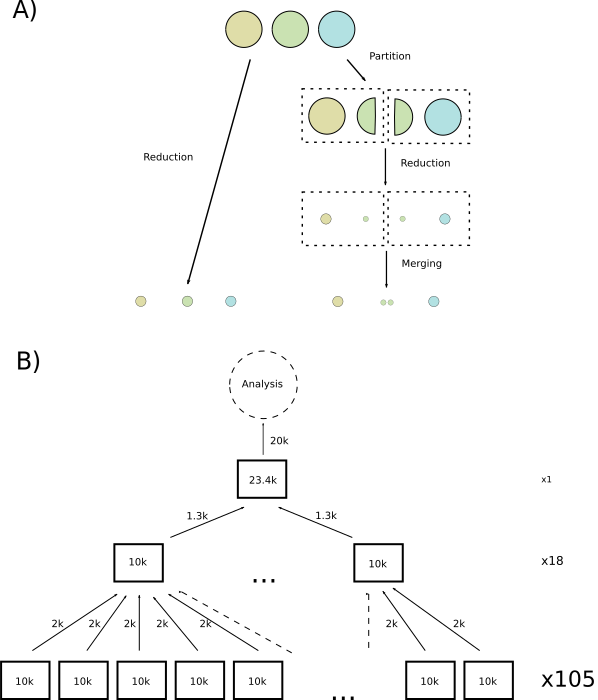
\includegraphics[width=\textwidth,height=\textheight,keepaspectratio]{pyproct_supp_compression.pdf}

\caption{A) Global reduction of the size of the dataset vs. merging local reductions. B) Different levels of compression including the number of frames used in each level.}
\label{fig:compression}
\end{figure}

The goal of this technique is to reduce the input trajectory by exchanging
sets of similar conformations (clusters) by a choice of its most representative
structures so that the final number of elements is proportional to
the original size of the cluster.

The first step to apply the reduction is to produce a clustering.
This makes us face the memory problem mentioned before. A workaround
for this issue is to divide the trajectory into smaller parts so that
each distance matrix can fit in memory, process each part separately
and then merge them again. Unfortunately, arbitrarily partitioning
the trajectory can separate elements that could form part of the same
cluster (which is more prone to happen in the boundaries of each part).
This can lead to an unevenness in the redundancy elimination process
(see the 2D example in Fig. \ref{fig:compression}A). We have performed
the reduction process iteratively to mitigate the problem. We start
with 105 parts of almost 10k frames each. After reducing each part
to 2k frames, we merged them into groups of 7 (\around14k
frames each). These groups were compressed to have around 1.3k frames
each and merged again to form a \around24k frames trajectory.
This was finally reduced to 20k frames and then analyzed. 


\subsubsection{Results}


\subsubsubsection{Performance}

pyProCT was run in an Intel Xeon CPU W3530 @ 2.80GHz workstation.
Each run of pyProCT spawned a maximum of 6 processes. While it was
being executed the workstation was normally used, occasionally triggering
operating system's swap mechanisms, which slowed down the process.
Therefore, the calculated execution time has merely a qualitative
meaning (see Table \ref{tab:results}). Also, the lack of knowledge of the
system forced us to use a very general hypothesis, increasing the
number of clusterings that had to be generated and thus the total
execution time. 

\begin{table}
\centering
\begin{tabular}{ r c c c }
\toprule
Level & Runs & Time per run (s) & Clusterings per run \\
\midrule

Third (10k$\rightarrow$2k) & 105 & \around1500 & 300-400\\
Second (20k$\rightarrow$1.3k) & 18 & \around2200 & 300-400\\
First (24k$\rightarrow$20k) & 1 & 12395 & 452\\
\bottomrule

\end{tabular}
\protect\caption{Around 40k clusterings were produced in almost 58h (1 clustering each
5s).\label{tab:results}}
\end{table}

\subsubsubsection{Clustering}

The clustering chosen by pyProCT was composed of a total of 19 clusters,
one of them holding the 34\% of the conformations. The C$\alpha$-RMSD
with the experimental structure (PDB id 2JOF) is 1.8${\AA}$, which
is similar to the 1.4${\AA}$ RMSD calculated in the original article
(see Fig. \ref{fig:clusters}). 

\begin{figure}
\includegraphics[width=\textwidth,height=\textheight,keepaspectratio]{pyproct_supp_clusters.png}

\protect\caption{Representative conformations for the 4 most populated clusters, holding
a 34\%, 13\%, 8 \% and 8\% of the elements of the dataset. \label{fig:clusters}}
\end{figure}


\subsection{2D Validation}
\label{sec:pyproct_supp_6}

In order to improve the reliability of pyProCT we have performed two
different quality assurance methods. The first was to ensure that
the software itself was working correctly using a unit testing methodology
(trying to get the best possible test coverage). The second was centered
in the validation of the clustering algorithms and the protocol.

Clusterings are hard to validate, especially when using
multidimensional data. Validating a 2D clustering, however, can be
an easier task as it can be visually checked. To this end we coded
the scripts that can be found in the folder\texttt{ pyproct/validation/bidimensional/}.


\subsubsection{Datasets}

To perform the validation, we downloaded some of Helmuth Spaeth's\cite{spaeth_spaeth_????-1}
datasets. These datasets have different characteristics that make them
difficult to cluster : 
\begin{enumerate}
	\item In this dataset 3 to 5 clusters can be seen. It looks like some of
	them can be subdivided. In general, these clusters are compact.
	\item It shows a set of points homogeneously covering the plane. There is not noticeable
	density variations.
	\item In this case there are two different density regions. In the bottom-right
	corner there is a compact cluster. The remaining points are sparsely
	distributed in the remaining space .
	\item Two compact clusters to the left, one big cluster (which seems to
	be composed of other clusters) sits on the right.
	\item Three parallel elongated clusters of different sizes and densities.
	\item Three elongated clusters with similar densities sharing the same origin.
	\item Two overlapped elongated clusters with different densities.
	\item Three elongate clusters with similar densities. All three are overlapped.
\end{enumerate}

We also used a code adapted from Jochen Wersdrfer's blog \cite{wersdorfer_spectral_????}
to generate a 9th dataset, which contains 450 points lying in three
concentric circles.


\subsubsection{Protocol validation}

In the first version of the validation script we used the datasets
to validate the algorithms, that is, we coded some algorithm-parameter
pairs and checked a picture of the resulting clusterings. Since the
algorithms were working as expected, we upgraded the script to fully
test the HCE protocol.

For each dataset, two hypotheses about the noise, cluster size and
number of clusters were defined (see \ref{tab:description_table})
based on our observations of the datasets. Also, we used two different
criteria to describe the expected clusterings:

\begin{description}
	\item [``default\_criteria''] Uses Silhouette and Cohesion ICVs. Is
	the default criteria of pyProCT and fosters both separation and compactness.
	\item [``graph\_criteria''] Uses the 'NCut' ICV. It tries to separate
	a graph representation of the dataset into connected components so
	that the sum of inner edge weights is optimized.
\end{description}

\begin{figure}
	\includegraphics[width=\textwidth,height=\textheight,keepaspectratio]{pyproct_supp_c_plots}

	\protect\caption{Results of the application of pyProCT to nine 2D datasets. Clusters
	are plotted using different colors and symbols.\label{fig:plots_2d}}

\end{figure}

\begin{table}
\centering
\begin{tabular}{ c c c c c c }
\toprule
Dataset & \specialcell{Min.\\Clusters} & \specialcell{Max.\\Clusters} & \specialcell{Min.\\Cluster Size} & \specialcell{Max.\\Noise} & Criteria\\
\midrule
1 & 2 & 10 & 3 & 10\% & ``default\_criteria''\\
2 & 2 & 10 & 2 & 10\% & ``default\_criteria''\\
3 & 2 & 10 & 10 & 10\% & ``default\_criteria''\\
4 & 2 & 10 & 8 & 10\% & ``default\_criteria''\\
5 & 3 & 10 & 10 & 5\% & \specialcell{``default\_criteria'' \\ and ``graph\_criteria''}\\
6 & 3 & 10 & 13 & 10\% & ``graph\_criteria''\\
7 & 2 & 10 & 10 & 10\% & \specialcell{``default\_criteria'' \\ and ``graph\_criteria''}\\
8 & 3 & 8 & 5 & 10\% & \specialcell{``default\_criteria'' \\ and ``graph\_criteria''}\\
9 & 3 & 4 & 100 & 5\% & ``graph\_criteria''\\
\bottomrule
\end{tabular} \protect\caption{Clustering hypothesis for each of the datasets.\label{tab:description_table}}


\end{table}

\begin{figure}
	\fittopageimage{pyproct_supp_concentric_circles}

	\protect\caption{An incorrect choice of the ICVs to express the desired resulting clustering
	traits can drastically modify the results. In this case the criteria
	was changed from ``graph\_criteria'' to ``default\_criteria'',
	favoring one of the clusterings generated by the K-Medoids algorithm.
	\label{fig:concentric_circles}}
\end{figure}


\subsubsection{Results}

Clusterings 1, 3, 4, 6 and 9 are in full accordance with
our expectations (see table \ref{tab:results_table} and Fig. \ref{fig:plots_2d}).
We thought that the optimum solution for dataset 2 could be to use
one single cluster encompassing all elements. However the final partition
in 5 clusters looks reasonable. 

Clustering 5, 7 and 8 are different of what our intuition dictates.
The main problem that pyProCT has when dealing with a dataset like
7 or 8 is that their ``natural'' clusters overlap i.e. there are
elements that belong to more than one cluster at the same time. This
could be overcome by adding fuzzy algorithms to the algorithms pool.
Despite this, results would look counterintuitive in any case, as its usefulness
in most scenarios implies to discretize the membership values.

Clustering 5 highlights a weakness of the HCE methodology: its success
depends on the ability of the user to convey their goals in the clustering
hypothesis. If the user is not able to express it using pyProCT built-in
ICVs (see Fig. \ref{fig:concentric_circles}) or the needed ICVs to define
the hypothesis are not yet implemented, it would be impossible for
users to get the best-fitted result for their problems. It is clear
that, in this case, none of the used criteria suffices to choose the
type of result we would like to obtain.

\begin{table}
\centering
\begin{tabular}{ c c c c c }
\toprule
Dataset & Algorithm & Num. Clusters & Noise & Criteria\\
\midrule
1 & Gromos & 4 & 8.10\% & ``default\_criteria''\\
2 & Spectral Clust. & 5 & 0\% & ``default\_criteria''\\
3 & K-Medoids & 2 & 0\% & ``default\_criteria''\\
4 & K-Medoids & 6 & 9.59\% & ``default\_criteria''\\
5 & K-Medoids & 3 & 0\% & ``graph\_criteria''\\
6 & DBSCAN & 3 & 4\% & ``graph\_criteria''\\
7 & K-Medoids & 2 & 0\% & ``graph\_criteria''\\
8 & K-Medoids & 3 & 5.19\% & ``graph\_criteria''\\
9 & Spectral Clust. & 3 & 0\% & ``graph\_criteria''\\
\bottomrule
\end{tabular}

\protect\caption{Details of the results. Last column indicates the criteria
that obtained the best score. \label{tab:results_table}}
\end{table}


\newpage
\cleardoublepage

\newpage

\chapter{Summary of the results}

In the present chapter, we aim to give a brief summary of the results obtained for each of the proposed objectives. A more detailed discussion of each of them can be found in the next chapter.

\section{Technical improvement of PELE}

As stated before, the results related to the first objective consists, mainly, in the production of new software, which is not open source. The code base includes the rewriting of PELE in C++, the related Python scripts, and the parallelized kernels. 

As one of the main objectives of this thesis is the development of faster sampling techniques for VHTS, a significant amount of work was focused on speeding up the software. This was partly achieved by GPU acceleration of the heavier routines, where we obtained up to 24x kernel speedups. 

\section{Algorithmic improvement of PELE}

We have presented a new perturbation method for PELE using torsional normal modes (icNMA). We have tested the new methodology in two different systems (ubiquitin and an Src Kinase) and compared the results of the current method (ccNMA) and the new method with molecular dynamics simulations in explicit solvent. The results show that this approach is able to produce more energetically favorable perturbations than the Cartesian coordinates-based method, thus allowing to work at 300 K without the need of a system-wide minimization. The root mean square fluctuation of the residues indicates that icNMA reproduces protein flexibility better than ccNMA; however both fluctuate less than MD. The measurements of the solvent accessible surface and radius of gyration show that icNMA is able to better capture the variations of volume of the protein. Furthermore, the way it simulates the inter-domain movements of the Src kinase is more similar to MD. Finally, each icNMA iteration is faster than a PELE iteration, as it does not include the side chain prediction and global minimization steps.

Some parts of the icNMA code are open source and can be found in its GitHub repository\footnote{\url{https://github.com/victor-gil-sepulveda/PhD-ANMInternalCoordinates}}.


\section[Efficient and reliable analysis]{Efficient and reliable analysis of large conformational ensembles }

\subsection{Implementation of an efficient solution for the calculation of collective superimposition operations}
We have introduced the Python package pyRMSD. It provides the Python programmer with three superimposition algorithms and up to 4 fully parallelized collective operations. One of the examples shown, the calculation of an RMSD matrix, reaches a speedup of 5x when using 6 cores and 11x using a GPU.

The code of pyRMSD is open source (under MIT license) and, to the best of our knowledge, it is the first open source CUDA parallelization of this kind. Readers interested in downloading or contributing to the code can find it in its GitHub repository\footnote{\url{https://github.com/victor-gil-sepulveda/pyRMSD.git}}. Moreover, some compiled packages are hosted in the PyPI package repository\footnote{\url{https://pypi.python.org/pypi}} and can be easily installed using the \texttt{pip}\footnote{\url{https://pip.pypa.io/en/stable/}} tool, which manages the downloading, compilation, installation and the handling of dependencies.


\subsection{Implementation of a reliable cluster analysis protocol}

We have presented the Python software pyProCT which aims to be a reliable cluster analysis alternative when used as a black box. We have described how the meta-algorithm works and shown some of its features in two representative use cases. In the first one, we have been able to correctly separate the conformations of two synthetic conformational ensembles without any knowledge of their generation process. Moreover, an iterative analysis method to refine the working hypothesis has been introduced. 
In the second use case, we have used pyProCT to eliminate the redundancy of a large DNA-ligand simulation and obtain the best ligand clusters. Our results correlate well with the clusters obtained in previous works using a kinetic analysis. Finally, we have shown how pyProCT can be used to reduce the size of a huge conformational ensemble (around 1 million structures) to find the most biologically relevant conformations of a protein folding simulation. 

On the technical side, pyProCT also takes advantage of parallel architectures (multicore or distributed architectures) by using a parallel task scheduler. The code is also open source (under MIT license) and can be found in its public GitHub repositories\footnote{\url{https://github.com/victor-gil-sepulveda/pyProCT} and \url{https://github.com/victor-gil-sepulveda/pyProCT-GUI}}. Both pyProCT and its GUI are also available in the PyPI repository and can be installed easily using the \texttt{pip} tool.

\newpage

\newpage

\chapter{Discussion}

\section{Technical improvement of PELE}

\subsection{From PELE to PELE++}

On its previous incarnation, PELE was using the functions of the Protein Local Optimization Program (PLOP)
\cite{jacobson_role_2002} software package as a library. Since PLOP had been written in FORTRAN
77-95, the most natural choice for PELE was to use the same programming language. The limitations of FORTRAN, together
with the pragmatic but chaotic nature of academic developing, drove it to a maintainability dead-end. The refactoring
needed to pay the accumulated ``technical debt'' was so huge that we decided to go through a complete rewriting of the code . 

The author of these lines worked on this rewriting steadily for two years and a half, making more sparse contributions since then, and was in charge of the design of the software core and of its successive iterations. Given the magnitude of the
project, a small group of technicians soon joined the development team which was leadered by Mr. Manuel Rivero Gonz\'alez
for more than three years. This group has been renewed lately, and is now leadered by Dr. Jorge Estrada. The rewriting
has been named PELE++ and has been the base of all the developments mentioned in this work.

The old version of PELE  was an academic software, and so is PELE++. This means that the software was not only planned to be used to
perform \textit{in silico} experiments but also as a tool to test and develop new algorithms. As a consequence, the new code
needed to be well documented, easy to learn, easy to maintain and robust to experimental changes. The academical nature
of the software, indeed, explains some of the design decisions taken. As a result, PELE++:

\begin{itemize}
\item Uses an Object-Oriented Programming (OOP) paradigm instead of the previous single file per module approach, which also fosters
reusability. C++ has been chosen as the language for this new version as it implements the OOP paradigm and compiles to
very efficient executables.
\item Is better designed for maintainability: Design patterns and other Software Engineering techniques have been
wittingly applied (see Fig. \ref{fig:pele_core_uml}). SOLID\footnote{Acronym for Single responsibility principle,
Open/closed principle, Liskov substitution principle, Interface segregation principle and Dependency inversion
principle} principles have been honored. As a side effect, testability has been improved.
\item Is better documented: The constant turnover of new students has made it necessary to pay special attention to a proper
documentation of code functions and classes. This shortens the time needed to train new developers so that they can
start  to contribute to the project earlier. 
\item Is more reliable: the code correctness can be tested at any phase of the project. An in-house testing library was
coded, and each class owns a test suite. An automated testing protocol was implemented. 
\item Has better performance than the old version: several algorithms were replaced with more readable and efficient
alternatives.
\item Is easier to extend and modify, a desirable feature as many people would use the code to test their own algorithms.
\end{itemize}

To exemplify the design changes provided, we include here a simplified UML (Unified Modelling Language) diagram (see Fig.
\ref{fig:pele_core_uml}). The diagram shows two packages: the first describes the handling of structural
data, while the second models the energy calculation subsystem. We have chosen to neglect several minor classes and
methods for the sake of clarity. We can observe how creation patterns have been profusely used in this new design: the
Builder pattern for Potential objects, the Simple Factory pattern for ForceField objects. Consider that the
Abstract Factory pattern, used to create the diverse AtomSet descendants, is not shown here. 

The AtomSet object, a group of atoms with defined geometry (coordinates) and topology (interactions), is of particular interest as
it is involved in two different hierarchies. The first one is semantic and comes from the use of inheritance (e.g. a
Residue is a type of Link which is a more general case of an AtomSet). The second one reveals a tree-like organization
that emerges from a loose interpretation of the Composite pattern: the root is the Complex, a singleton object made of Chains which, in turn, are  made of Links. 

The rewriting of the code has allowed us to add new features to PELE, such as the possibility of using different force fields and various solvent models, supporting the simulation of other biopolymers (e.g. DNA
\cite{cabeza_de_vaca_new_2015}), using arbitrary sized structures and coarse-grained models and
even performing an effective parallelization of the code. In general, this has converted PELE in a tool that is more useful for
academical experimentation and efficient and reliable enough for industrial use. 

\subsection{Performance vs. maintainability}

Scientific software is the object of an open debate on performance versus readability. The development of PELE++ has shown us
that fostering readability can save developers time and efforts at almost no performance cost, in contrast with the theories supported by other authors  \cite{larsson_algorithm_2011}. Readable code, for
instance, allows building a better structured code base. Thanks to this, developers can have a better global view of the
software and apply optimizations (e.g. avoid unnecessary actions). It also allows them to react faster in front of
specification changes and augments the resiliency of the developing team to staff adjustments. 

One of the most important issues we faced is the mutability of specifications, in spite of the thorough initial use case studies. This
can be caused by the communication gap between developers and users (or stakeholders), due to their different domains of
knowledge. As this situation can pose a great problem for long-term design, we consider that domain-driven design techniques,
using experts' feedback to refine the model, might be of great help. 

Finally, this development has taught us that,
in order to succeed in such big projects, it is important to perform short and abundant refactoring cycles and,
ideally, to assign development tasks to optimal-sized teams of specialized software engineers.

\begin{sidewaysfigure}
    \centering

\fittopageimage{PELEppcore}

\caption{Pseudo-UML diagram showing the most relevant classes in PELE++ core: the AtomSet tree which
allows the definition of different types of molecules, the topology subsystem and the energy/potential subsystem. The
last uses geometry (atom coordinates) and topological information to calculate the energy of an AtomSet.}

\label{fig:pele_core_uml}

\end{sidewaysfigure}

\subsection{Optimization and Parallelization}

During the last decade, Moore's law predictive power has  reached its limits, since semiconductor manufacturers have found the
physical limits of miniaturization; CPU frequency scaling beyond that point was not
possible and, as a consequence, cluster-based computers were the only solution left to increase the global
computational power. This was undoubtedly the starting shot for the development of multicore CPUs in commodity
hardware. Some years later, the graphic coprocessors of such CPUs evolved to standalone graphic cards
(GPUs\footnote{Graphics Processing Unit}), which manycore chips were eventually adapted to perform highly parallel
computations. Soon after, Intel presented their MIC\footnote{Many Integrated Core} architecture. Easier to program
than GPUs and also able to perform highly parallel computations, it has rapidly become as prominent as GPUs were some years
ago. Computational hardware evolves rapidly, and software must be able to take advantage of this evolution.

One of the improvements of the PELE rewriting has been offering a code base that can be parallelized more easily than the old
FORTRAN version.

\subsubsection{Initial profilings}

\begin{table}
\centering
\begin{tabular}{ c c c c } 
\toprule
~ & \multicolumn{2}{c}{Protein}  & Ligand \\
\cline{2-4}
Size &  Residues &  Atoms &  Atoms\\
\midrule
Small & 120 & 1731 & 19\\
Medium & 583 & 9300 & 16\\
Big & 710 & 11222 & 45\\ 
\bottomrule
\end{tabular}

\caption{Size-related details of the systems used in the initial profilings.}
\label{table:profile_sizes}
\end{table}

We selected three real (under study) protein-ligand systems with different sizes to use them in our test simulations. The
number of atoms and residues of such systems is summarized in Table \ref{table:profile_sizes}. 

The initial profilings used the two currently implemented implicit solvent models in order to identify  the
most efficient one. Executions were performed in a Mare Nostrum \cite{barcelona_supercomputing_center_marenostrum_2015} node (Intel
SandyBridge-EP E5--2670 @2.6 GHz processor). Nodes were used exclusively so that no other
processes could interfere with the results. A control script was written for each of the systems and solvent models, and
PELE++ was run for 100+ steps in order to enter the convergence regime. The profiling was performed using the same
script for ten steps, being the initial conformation the last frame of previous simulations. Profiling data was then
extracted using gprof \cite{graham_gprof_1982} and then analyzed using the visual analysis tool
gprof2dot\footnote{https://github.com/jrfonseca/gprof2dot}. 

\begin{figure}

\fittopageimage{initialProfiling}

\caption{A set of profiles was performed for different protein sizes and using OBC and SGB solvent. This bar plot shows the percentage of time spent in non-bonding and solvent-related calculations.}

\label{fig:first_profile}

\end{figure}

The results showed that PELE++ spent most of the time in two kinds of functions (see Fig.
\ref{fig:first_profile}):

\begin{itemize}
\item Functions related to the solvent model, more specifically the alpha and surface elements. It is worth noting
that simulations using the OBC solvent model were typically faster. 
\item Functions related to the calculation and the evaluation of non-bonding lists in order to calculate the
electrostatic and van der Waals potential energy terms and gradient. This is common in MD, among other methods, and has been
the topic of several other studies \cite{myung_accelerating_2010, schmid_gpu_2010, jin_cuda_2011}. 
\end{itemize}
From this profiling exercise, we also learned that the behaviour of PELE++ can totally change depending on the place of
the ligand. Two different scenarios were identified: free ligand diffusion (the ligand explores the protein surface freely) and binding refinement (the ligand is already in the binding site, and a better pose is searched).

\subsubsection[Non-bonding energy parallelization]{Non-bonding energy parallelization using GPUs}

According to the profile results, the next logical step would have been improving the performance of the solvent-related
functions, but the difficulty of parallelizing the SGB\footnote{First attempts were made at an early stage of the
code, when OBC solvent was not yet available. } algorithm (due mainly to its data dependencies) lead us to focus on
the performance improvement of NB functions first \cite{oro_gay_parallelitzacio_2012}.

The main contribution of NB energy/gradient calculations to the overall time does not reside in the computational cost
of evaluating a single interaction calculation, which is indeed quite fast, but in the huge number of calculated interactions ($\propto N^2$ where $N$ is the number of atoms). 

The evaluation of these huge lists of interactions looked to be a computationally-bound problem and fit well with the
GPGPU (General-Purpose computing on Graphics Processing Units) paradigm. Graphic Processing Units have many core
architectures with numerous parallel calculation units that allow them to perform high-throughput calculations with ease.
They usually have good bandwidth but elevated latencies, which can be shaded thanks to the extensive use of lightweight
threads that allow alternating calculations with memory operations. 

We wanted to adapt PELE++ code to work with this kind of accelerators using the OpenCL (Open Computing Language) and
CUDA (Compute Unified Device Architecture) programming models. The first step was to design two new structures to pack
the data that would eventually be sent to the device. Afterwards, we coded the GPU kernels for the energy and gradient
calculations. The energy case is quite trivial, as each thread just calculates several NB interactions to a
per-thread accumulator variable. The final value of the energy is calculated through a reduction of the partial energy
values. 

Conversely, parallelizing the NB gradient calculation using a GPU is not that easy. The fundamental problem is that all
threads can potentially end writing in the same positions of the gradient (race condition) and regular strategies to
protect concurrent access would only end penalizing performance noticeably. To illustrate this, the reader can think of
three particles A,B and C so that particle A interacts only with particle B, and B with C. If two different threads are
calculating AB and BC interactions, it is very likely that both try to access B's gradient positions at the same time. 

The solution starts by storing the gradient partial contributions in one temporary array. As the gradient contributions
of each atom in the interaction pair are equal but opposite, it is possible to use only half of the memory to store
intermediate results. Once all the interactions are evaluated and the array is filled, it is  ordered by atom using
two mapping tables (one for each interacting atom) so that each GPU thread is able to reduce all the iterations of one atom
at a time.

In order to test our code, we had two different GPUs available: an NVIDIA Tesla M2090 card (for CUDA implementation only)
and an AMD Radeon HD 6870 card. Both cards have different technical specifications\footnote{E.g. Nvidia card has 512
threads per block and the AMD card has 256 and no double precision support} and their results are not
comparable. Another set of three proteins with a larger number of atoms was used with \around 1k atoms, \around 14k atoms and
\around 30 atoms so that the calculation times of a single non-bonding list were significant.

Our first estimates showed that the calculation of kernels was so fast that transference and precalculation overheads were
making the overall performance worse than the serial version. Both data transfer and kernel execution were made asynchronous, thus
alleviating the relative impact of that overheads. 

The comparison of performance results was made at kernel and program levels. The execution time of serial and GPU
kernels (Fig. \ref{fig:cuda_speedup}) showed speedups of up to 24x for the energy function and 12x for
the gradient.

\begin{figure}

\fittopageimage{cudaKernelSpeedup}

\caption{Comparison of the energy and gradient functions speedup for different protein sizes and the two
programming models used. One of the reasons why the speedup for the medium protein is higher is because the relative
weight of the non-bonding calculations has increased with the number of atoms.}

\label{fig:cuda_speedup}

\end{figure}

At that time, the code was not mature enough to introduce the changes that would allow serial and accelerated versions
to coexist. In order to obtain values for the execution of the whole program, we had to build a model of its behaviour based on the profiling studies, typical executions and our knowledge of the code.

The Truncated Newton minimization is the part of the code where energy and gradient functions are called the most. The
method consists in several iterations of a five stage protocol \cite{xie_remark_1999}, called the ``outer
loop'', which includes some preparatory steps and the evaluation of the Hessian. The ``inner loop'' is the stage in
which a preconditioned conjugated gradient is performed. Each minimization is usually run three times with fixed alpha
values\footnote{Atomic property regarding the solvation model.} for performance reasons. The time needed to perform a
minimization in the serial case can be modelled as:

\begin{equation}
T = 3 (N (t_5 + M t_5))
\end{equation}

and for the parallel case:

\begin{equation}
T = 3 (t_2 + N (t_1 + t_3 +t_4 +t_5 + M (t_1 +t_5 )))
\end{equation}

where $N$ and $M$ are the number of times the ``outer'' and ``inner loops'' are executed, $t_1$ and $t_2$ are
the time needed to create (if applicable) and transfer atomic data structures to GPU, $t_3$ is the time required to
generate the vector of interactions in the GPU, $t_4$ is the time needed to order the atom interaction maps and
$t_5$ is the time needed to calculate the gradient. It is worth mentioning that non-bonding calculations are to be
performed in both the ``outer'' and ``inner loops'', and that coordinates will be changed at each ``inner loop''
iteration, which makes it mandatory to update their GPU memory representation. 

The model allowed us to obtain a rough estimate of the execution of the whole program (Fig.
\ref{fig:cuda_global_speedup}) in the serial and parallel case. The results showed that adding the
CUDA implementation to PELE++ would imply a 16.3 - 27.8\% faster execution than the serial version. The expected
performance increase for the OpenCL code was smaller, with a 13.5 - 26.7\% speed increase. However, it is not possible
to make a fair comparison of both methods, as hardware platforms are not equivalent and, also, CUDA kernels are
using an optimized sorting algorithm from a library, while the OpenCL sorting algorithm had to be coded from scratch.

\begin{figure}

\fittopageimage{cudaGlobalTheoSpeed}

\caption{The global speedups have been calculated using a model. As parameters N and M range from 1
to 65 and from 20 to 50 respectively, we decided to study the best case (faster serial execution, where N = 1 and M
= 20) and the worst case (slower serial execution, where N = 65 and M = 50). Theoretical speedup increases to 
decrease afterwards. This happens as a result of the changes in the relative weight of the non-bonding calculations: the weight first
increases due to the increment in the number of atoms and then decreases since other functions, such as the covalent energy
calculations, start to require more time. The difference between implementations is not significative.}

\label{fig:cuda_global_speedup}

\end{figure}


\bigskip

\subsubsection{Solvent parallelization}

The performance improvement through the parallelization of solvent-related functions is currently an open project
lead by our research group's technicians Pedro Riera and Jorge Estrada, the company
Pharmacelera\footnote{http://www.pharmacelera.com/} and BSC's Montblanc\footnote{https://www.montblanc-project.eu/}
project team. The most costly functions are the ones that calculate surface elements and atom alpha attributes (which
are used when calculating energy in order to take solvation contributions into account).

As mentioned before, there are currently two different solvent models included in PELE++, namely, the SGB
\cite{ghosh_generalized_1998} and OBC models \cite{onufriev_exploring_2004}. The
algorithm for the SGB alpha calculation function is detailed in the pseudocode below:


\begin{lstlisting}[caption = {}, label = {}, mathescape=true,escapeinside={(*}{*)}]
updateAlphasSGB:
	updateSurfaceElements $O(R n^2)$
	updateAtomAlphas $O(n)$
	updateSASA $O(R n^2)$

\end{lstlisting}

The calculation of the atom alpha property depends on the previous calculation of the surface elements. This is the most
costly function, since it depends  on the number of atoms, their neighbours and a resolution parameter (a worst-case complexity
of $O(R n^2)$).

\begin{lstlisting}[caption = {}, label = {}, mathescape=true,escapeinside={(*}{*)}]
updateAlphasOBC:
	for each atom:
	ComputeOtherAtomsContribution $O(n)$
\end{lstlisting}

The OBC alpha updating method is implemented as a double loop over all atoms (a complexity of $O(n^2)$) which makes
it simpler than SGB's (and thus easier to parallelize) and explains why its serial performance is better.

\subsubsubsection{Solvent parallelization: OpenMP}

Some initial attempts of parallelizing the SGB alpha calculation functions were performed using the OpenMP programming model.
Two functions were selected: \texttt{computeSurfaceElementsOfAtom} ($O(R n)$) and \texttt{updateAtomsSurface} ($O(n^2)$) both called by
the \texttt{updateSurfaceElements} function. 

Tests were performed using a medium size system (4284 protein atoms and 69 ligand atoms) and an Intel SandyBridge-EP
E5--2670 (@2.6 GHz) processor. The best results were obtained using eight threads and threw overall speedups of \around1.5x for
the refinement and free ligand diffusion simulations. \ignore{hl{los resultados no tienen en cuenta
que el NB tb este paralelizado, por otro lado se tendra que ver si, en el segundo caso, hay error de medida ya que el
speedup es del orden del speedup maximo teorico, aunque Pedro dice que no}}

\subsubsubsection{Solvent parallelization: OpenCL}

The parallelization of SGB solvent functions has been currently abandoned in favour of OBC functions due to their
greater simplicity and better serial performance. Pharmacelera engineers have focused on parallelizing it using the
OpenCL programming model and have devised 3 parallelization strategies:

\begin{itemize}
\item Parallelization of the inner loop (\texttt{ComputeOtherAtomsContributions} function) (method 1).
\item Parallelization of the outer loop (\texttt{updateAlphas} function) (method 2).
\item Precalculation of atom pairs and parallelization over these pairs (method 3).
\end{itemize}

The first and second strategies have a lower impact on the code, while the third makes a better use of the GPU by improving the
load balance. 

The tests have been performed on a workstation equipped with an AMD FirePro W5100 GPU card. The results, using the
medium and big size proteins employed in the initial profilings, are promising, especially in the case of the third
strategy which seems to have the best performance (see Fig. \ref{fig:solvent_speedup} ).

\begin{figure}

\fittopageimage{pharmaccelera_speedup}

\caption{Kernel speedup for each of the methods and proteins tested. Methods 2 and 3 seem to obtain an equivalent efficiency improvement. }

\label{fig:solvent_speedup}

\end{figure}

\subsubsection{Montblanc and other projects }

Nowadays, the main obstacle to projecting Exascale systems is energy consumption. The Montblanc project aims at the
creation of an energy-efficient and scalable supercomputer using ARM\footnote{Advanced RISC (Reduced Instruction Set
Computing) Machine} technology. Some of the parallelization techniques explained before are currently being tested in
this novel architecture.

Finally, some parts of the code are currently being ported to the CUDA programming model as part of the CUDA Center of
Excellence program from NVIDIA.

\newpage




\newpage
\cleardoublepage
\section{Algorithmic improvement of PELE}

Most of the limitations of PELE enumerated in the introduction (Section~\ref{sec:anm_limi}) are common to all methods using NMA or more specifically ANM, and therefore not exclusive to PELE. Some of the issues are related to the NMA model itself, while the rest are related to the specific ways normal modes are applied. This made us think that finding an alternative to the NMA algorithm would produce a noticeable improvement in PELE sampling robustness and performance. To this end, we have chosen to implement an internal coordinate (IC) based NMA.

\subsection{Switching to a different coordinates space} 

Internal coordinate NMA (icNMA) is not a novelty. Indeed, the pioneering NMA works of Wilson \cite{wilson_molecular_2012} were already performed in the internal coordinates space. This is not surprising, given that internal coordinates (e.g. bond distance, bond angle, and dihedral torsion angles) are the most natural way of representing chemical molecules (e.g. with a z-matrix \cite{gordon_approximate_1968}). Actually, several methods use internal coordinates instead of Cartesian coordinates. Some examples are the Multiple Minima Monte Carlo \cite{li_monte_1987} method, the Monte Carlo sampling software MCPRO (Monte Carlo for PROteins) \cite{jorgensen_molecular_2005} and ICM \cite{abagyan_icm_1994}, or the MD software X-PLOR \cite{stein_torsion-angle_1997} and DYANA \cite{guntert_torsion_1997}.

The truth is that Cartesian coordinate NMA methods (ccNMA) are more common than icNMA-based methods, possibly because the mathematical background of the former is more simple. However, this fact has not prevented researchers from introducing icNMA in their simulation software. First examples can be found in the early works of Noguti \textit{et al.} \cite{noguti_method_1983, noguti_efficient_1985} and Kidera \textit{et al.} \cite{kidera_enhanced_1995,kidera_smart_1999} where the  scaled collective variables (SCV) MC and related algorithms are presented. Trosset  \textit{et al.} used later a similar methodology \cite{trosset_prodock_1999} in the implementation of PRODOCK. Levitt and Stern \cite{levitt_protein_1985} suggested an MD method using IC NMA modes. Finally, Lin and coworkers \cite{lin_evaluating_2011} developed a different method using icNMA followed by an energy minimization. 

There exist reports claiming that a significantly smaller number of modes are needed to reproduce conformational changes using torsional NMA \cite{bray_optimized_2011}, and that this method improves sampling quality \cite{mendez_torsional_2010-1} and the results of ligand binding simulations \cite{kovacs_conformational_2005} compared to ccNMA-based methods. Changing the coordinate system  implies not only changing the way normal modes are calculated, but also the way modes are applied, which could help to mitigate many of the NMA-related issues.

\subsection{Coarse grain model}
The CG model used in our icNMA implementation describes rigid units that encompass all the heavy atoms among rotatable backbone torsions ($[C_\alpha]^3$ \cite{ghysels_mobile_2009, ghysels_comparative_2010} model). This means that we will define \around$2R$ units for each chain (where $R$ is the number of residues), which can be of 4 different types (see Fig. \ref{fig:icNMA_CG}):

\begin{description}
\item [N-terminal unit] Contains the N-terminus, \calpha and first residue side chain.
\item [\calpha unit] Contains the \calpha atom and side chain.
\item [C-terminal unit] Contains the atoms that form the final carboxyl group.
\item [Peptide bond unit] Contains the carboxyl and amino groups involved in the peptide bond.
\end{description}

To account for the rigidity of the $\phi$ torsion in prolines, its peptide bond and \calpha units will be fused together (see Fig. \ref{fig:icNMA_CG}B).

\begin{figure}
\fittopageimage{CoarseGrainModel}
\caption{CG model of a peptide (A) using the $[C_\alpha]^3$ distribution of atoms. Each residue is composed of two units which are delimited by the $\phi$ and $\psi$ torsions. The case of proline residues (B) is special, as they only form one unit.}
\label{fig:icNMA_CG}
\end{figure}

\subsection{icNMA theory}

\subsubsection{Hessian calculation}

\begin{figure}
\fittopageimage{VectorialNotationANMIC}
\caption{Representation of the rotation of two rigid bodies (green and purple) around axis $q_{\alpha}$.}
\label{fig:icNMA_bodies}
\end{figure}

Again, we model our system as a spring network whose potential is the sum of all Hookean interactions between atoms (or CG units) with the form $Vij = \frac{k_ij}{2} (r_{ij} - r_{ij}^0)$\footnote{As a convention, units and dihedrals will be numbered correlatively from N-terminal to C-terminal. Regular letters will be used to index atoms and units, and Greek letters to index dihedrals.}. If we express these interactions using generalized internal coordinates (which in our case will be limited to the torsion angles of backbone dihedrals), we can write the potential energy as:

\begin{equation}
V = \frac{1}{2} (q - q^0) H (q-q^0)^T
\end{equation}

and the Hessian in terms of $q$ \cite{kovacs_conformational_2005} as:

\begin{equation}
H_{\alpha,\beta} = \frac{\partial^2 V }{\partial q_\alpha \partial q_\beta} = \sum_{i<j} \frac{f_{ij}}{ \left| r_{ij} \right|^2} \left< r_ij , \frac{\partial r_i - \partial r_j}{\partial q_\alpha} \right> . \left< r_ij , \frac{\partial r_i - \partial r_j}{\partial q_\alpha} \right > 
\end{equation}

which depends on the values of the inverse of Wilson's $B$ matrix \cite{wilson_molecular_2012} ( with elements $\frac{\partial r_i}{\partial q_\alpha}$). If we impose Eckart conditions \cite{eckart_studies_1935} ($\sum_i m_i \frac{\partial r_1}{\partial q_\alpha} = 0$  and $\sum_i m_ir_i^0 \times \frac{\partial r_1}{\partial q_\alpha} = 0$ ) and that the origin of the molecule is the center of mass, the partial derivatives can be calculated as \cite{noguti_dynamics_1983}:

\begin{equation}
\frac{\partial r_1}{\partial q_\alpha} = e_\alpha \times \left( \frac{M_2}{M} r_\alpha + \frac{M_1}{M} r_1^0 \right) - r_1 \times \frac{M_1 r_1^0 \times (e_\alpha \times r_\alpha) + I_2 e_\alpha)}{I}
\end{equation}

\begin{equation}
\frac{\partial r_2}{\partial q_\alpha} = - e_\alpha \times \left( \frac{M_1}{M} r_\alpha + \frac{M_2}{M} r_2^0 \right) + r_2 \times \frac{M_2 r_2^0 \times (e_\alpha \times r_\alpha) + I_1 e_\alpha)}{I}
\end{equation}

which describes the change of Cartesian coordinates when one part of the chain is kept fixed and the other part moves around torsion $q_\alpha$ and vice versa. Both rigid bodies must be taken into consideration for a single rotation, as Eckart conditions imply the conservation of momentum. In these and in the following equations, $M$ is the summed mass and $I$ is the inertia tensor for all the units that compose the molecule. $M_1$, $M_2$, $I_1$, $I_2$, $r^0_1$ and $r^0_2$ are the summed masses, inertia tensor and center of mass of the set of units to the left (subindex $1$) or to the right (subindex $2$) of dihedral $q_\alpha$ ; $e_\alpha$ is a unit vector with the direction of the bond;  $r_\alpha$ and $r_{\alpha+1}$ are the positions of the atoms at both ends of the rotatable bond. Finally, $r_1$ and $r_2$ are arbitrary atoms in any of the left or right units of $q_\alpha$ torsion (see Fig. \ref{fig:icNMA_bodies}).

From these equations, a naive expression for the Hessian calculation can be deduced with a $\Theta (n^4)$ computational cost (assuming that the number of dihedrals is roughly proportional to the number of atoms). We are again in debt to Noguti and Go \cite{noguti_method_1983} and Abe and coworkers \cite{abe_rapid_1984} for the development of a recurrent method to calculate the Hessian, which can be implemented as a faster recursive algorithm ($\theta(n^2)$) that also turns out to be more memory efficient. First, Cartesian and internal coordinate-dependent terms are separated so that we can write each Hessian element as

\begin{equation}
H_{\alpha,\beta} = \left( e_\alpha, e_\alpha \times r\alpha \right) R_{\alpha,\beta} \left( \begin{array}{cc} e_\alpha \\\ e_\alpha \times r\alpha \end{array} \right)
\end{equation}

where the matrix $R$ is calculated as 

\begin{equation}
R_{\alpha,\beta} = \sum_i {\scriptscriptstyle \alpha} \sum_j {\scriptscriptstyle \beta} D_{ij}
\end{equation}

$D$ matrix models the interaction of atom $i$ and $j$:

\begin{equation}
D_{ij} = \frac{f_{ij}}{ \left| r_{ij} \right|^2} \left( \begin{array}{cc} r_i \times r_j \\\ r_{ij} \end{array} \right) \left( r_i \times r_j , r_{ij} \right)
\end{equation}

where the distance-dependent force constant is calculated as:

\begin{equation}
f_{ij} = \frac{k_0} { 1.0 + \left( \frac{r_{ij}}{x0} \right) ^6}.
\end{equation}

In our implementation, $k = 1$ and  $x0 = 3.8$, which are the same definitions used by the iNMA software \cite{lopez-blanco_imod_2011}.

To calculate the elements of $R$ we may need to store (or recalculate, which would affect computational efficiency) all $D_{ij}$ values. The number of matrices stored can be lowered by defining a matrix $T$, whose elements $T_{ab}$ summarize the interactions of all the atoms of rigid units $a$ and $b$:

\begin{equation}
T_{a,b} = \sum_{j \in a} \sum_{j \in b} D_{i,j}
\end{equation}

It is possible to calculate $R$ from $T$ by determining a new matrix $U$ so that:

\begin{equation}
U_{ab} = \sum_{i \leq a} \sum_{j >b} T_{ab}
\end{equation}

which contains all atomic interactions from the first unit to the $a$ unit, and from the $b$ unit to the last one (which can be interpreted as fixing units $a$ to $b$ and allowing units 0 to $a$ and $b+1$ to $M$ to rotate along dihedrals $\alpha = a$ and $\beta = b$). This makes it possible to calculate $R$ with only one index change: 

\begin{equation}
R_{\alpha,\beta} = U_{a,b+1}
\end{equation}

Finally, a recursive solution can be written so that:

\begin{equation}
U_{a,b} = U_{a,b+1}+U_{a-1,b} + U_{a-1,b+1}+T_{a,b}
\end{equation}

being the value of $U$ equal to 0 if any of its indexes is outside the range [0, $M$-1].


\subsubsection{Calculation of the metric tensor} 

We can also express the kinetic energy in terms of the generalized coordinates $q$ so that 

\begin{equation}
K = \frac{1}{2} \dot{q}^T K \dot{q}
\end{equation}

and the metric tensor K becomes

\begin{equation}
K_{\alpha,\beta} = \frac{\partial^2 K}{ \partial \dot{q}_\alpha \partial \dot{q}_\beta} = \sum_i^n m_i \left< \frac{\partial r_i}{ \partial q_\alpha} , \frac{\partial r_i}{ \partial q_\beta} \right>
\end{equation}


which can be calculated as \cite{noguti_dynamics_1983}:

\begin{equation}
\begin{split}
K_{\alpha\beta} = \frac{M_1 M_3}{M} \left[ e_\alpha \times (r_\alpha - r^0_1) \right] \left[ e_\beta \times (r_\beta - r^0_3)\right ] + \\ \left[ M_1 r_1^0 \times (e_\alpha \times r_\alpha) - I_1 e_\alpha \right] I^{-1} \left [M_3 r_3^0 \times (e_\beta \times r_\beta) - I_3 e_\beta \right]
\end{split}
\end{equation}


We are currently using the definition of the inertia tensor provided by Noguti and Go \cite{noguti_dynamics_1983}, also employed by Braun \textit{et al.} \cite{braun_formulation_1984} as defined by Lu and coworkers \cite{lu_new_2006} so that

\begin{equation}
I = \sum_i m_i P^T P
\end{equation}

and 

\begin{equation}
P_i = \left( \begin{array}{ccc} 0 & -z & y \\\ z & 0 & -x \\\ -y & x & 0 \end{array} \right)
\end{equation}

Once we have obtained the metric tensor and the Hessian, we can calculate the normal modes using Eq. \ref{eq:eigenproblem}. The resulting eigenvalues are still related to mode frequencies. The meaning of the eigenvectors, however, changes compared to their Cartesian coordinates counterparts; their size decreases from $3N$ to \around$2R$ (where $N$ is the number of atoms or CG units) and each single element $\alpha$ represents a differential rotation around torsion $q_\alpha$. 

In a preliminary study \cite{rincon_munoz_alisis_2014} we were able to demonstrate that the internal coordinate and Cartesian coordinate mode spaces are in good agreement.

\subsection{From internal to Cartesian coordinates and back} 

In order to compare IC modes with CC modes, we convert one coordinate system to the other using the Jacobian ($J$, inverse of Wilson's $B$ matrix) in the equation

\begin{equation}
J_{i,\alpha} = \frac{\partial r_i}{\partial q_\alpha}
\end{equation}

We can calculate Cartesian coordinate displacements from torsional rotations (and thus, from IC modes):

\begin{equation}
\Delta \vec{r}_{i,\alpha} = \sum_{\alpha}^N \vec{J}_{i,\alpha} v_i^\alpha  .
\end{equation}

We can also obtain torsional rotations from Cartesian displacements by using:

\begin{equation}
\Delta \Theta = (J^T M J)^{-1} J^T M \Delta r .
\end{equation}

\subsection{Description of the Internal coordinate NMA-based algorithm}
We have introduced a computationally affordable new IC NMA-based algorithm that aims at providing a fast traversal of the conformational space. The algorithm consists of two independent stages: the backbone perturbation and the side chain perturbation.

The backbone perturbation is implemented as an MC algorithm where each iteration comprises four steps:

\begin{enumerate}

\item  \textbf{Calculation of the target angular increments:} a normal mode and a sense for the rotations is randomly selected. The mode is scaled so that the maximum rotation amplitude is inside a user-defined range. The user can chose to specify a maximum ($a_{max}$) and a  minimum ($a_{min}$) value for the amplitude instead. In this case the maximum amplitude value is sampled from a truncated normal distribution with mean $\nicefrac{ (a_{min} + a_{max})}{2}$ and standard deviation $\nicefrac{(a_{min} - a_{max})}{4}$. Normal modes are calculated only at the beginning of the first iteration.

\item \textbf{Application of the angular increments:} the geometry of the protein is updated using Choi's \cite{choi_updating_2006-1} quaternion method.

\item \textbf{Side chain relaxation:} the rotations in the previous step treat side chains as rigid bodies. This may introduce atom clashes that must be freed. To this end, the side chains with any atom involved in a steric clash are selected and minimized. Note that, as only side chains are minimized, the conformations with clashes involving backbone atoms will be discarded in the next step because of their high potential energy. 

\item \textbf{Acceptance criterion:} the Boltzmann criterion is tested and the new conformation is accepted or rejected. 

\end{enumerate}

The side chain perturbation is again implemented as an MC algorithm where, at each iteration, a side chain is randomly selected and modified. To change the side chain, its rotatable bonds are found and a random increment is applied to each of them. The new side chain conformation will be accepted or rejected depending on the result of the Boltzmann criterion.


\subsection{Alternative implementation}

We also worked on a solution that allowed us to fuse the icNMA step with PELE original scheme \cite{rincon_munoz_alisis_2014} (i.e. performing an icNMA step plus the relaxation phase). As in the regular PELE algorithm, the last minimization must be constrained so that the backbone proposal is maintained. In this case, we have applied harmonic dihedral constraints ($U_{\alpha}^c(q_\alpha) = \nicefrac{k}{2} (q_\alpha-q_\alpha^0)$) to a percentage of the most flexible torsions. Restricting the number of constraints makes it is easier for the minimizer to free backbone stress and it helps it to converge faster. The gradient and Hessian derivations have been calculated and translated to C using the symbolic algebra software Maxima \cite{maxima_maxima_2014}. This alternative was studied during the preliminary development stage providing analogous results to those of ccNMA (the protein was collapsing into a compact form). This lead us to conclude that minimizations had a role in the sampling bias. 

\section{Obtention of the best set of parameters}

To compare IC and CC methods, we first need to obtain the set of parameters that maximizes the performance of both method simulations. To this end, we chose the most relevant parameters for each method and analyzed how their changes were affecting performance.  

\subsection{Characterization of the NMA step}

We started by isolating the mode application procedure in both methods. The ccNMA step comprises two smaller substeps:
\begin{enumerate}
  \item The calculation of the translation vectors, which depends on the \calpha displacement factor parameter (\textit{displacementFactor} defines the maximum displacement for the \calpha atoms).
  \item The application of these translations through a minimization. The ``strength'' or ``intensity'' of this minimization depends mainly on two parameters, the force constant of the spring pulling the \calpha atoms (\textit{steeringForce}) and the root mean square of the gradient (\textit{MinimumRMS}) that modulates the convergence of the minimization. 
\end{enumerate}

In the icNMA case, the NMA step coincides with a whole iteration of the backbone perturbation stage, and is performed in two consecutive substeps:
\begin{enumerate}
  \item The calculation of the torsional increments, which depends on the displacement factor parameter (\textit{displacementFactor}, which, in turn, defines the maximum rotation of any backbone torsional angle).
  \item The application of the rotations, which has no parameter dependencies.
  \item The side chain relaxation step, which again depends on the root mean square of the gradient (\textit{relaxMinimRmsg}).
\end{enumerate}

Table \ref{tab:parameters} summarizes the parameters that govern both methods.

\begin{table}
\centering
\begin{tabular}{ r c c c  }
\toprule
Method  & Movement amplitude & \multicolumn{2}{c}{Minimization strength} \\
\midrule
CC & \specialcell{displacementFactor\\ (\angstrom)} & \specialcell{steeringForce\\ ($kT/\AA$)} &\specialcell{ MinimumRMS \\(\nicefrac{kcal}{mol \angstrom})} \\
~  & 0.25, 0.66, 1.08, 1.5, 1.92 & 20, 40, 60, 80, 100 & 0.01, 0.05, 0.1\\
  IC & \specialcell{displacementFactor\\ (radians)} & \multicolumn{2}{c}{\specialcell{relaxMinimRmsg\\(\nicefrac{kcal}{mol \angstrom})}} \\
~  & 0.02, 0.05, 0.075 ,0.1, 0.12, 0.15 & \multicolumn{2}{c}{0.01, 0.05, 0.1}\\
\bottomrule
\end{tabular}
\caption{Choice of parameters affecting the mode application step in the CC and IC methods, including the values that will be used in characterization tests.} \label{tab:parameters}
\end{table}

To characterize the results of each step, we have focused on three features:
\begin{itemize}
	\item The \calpha RMSD between the initial conformation and the conformation after the mode application step, which shows the extent of the backbone deformation.
	\item The increment of internal energy between the starting conformation and the conformation after the NMA step, which shows how likely this deformation would be.
	\item The time the step takes.
\end{itemize}

Ideally, a good set of parameters is the one that produces big RMSD displacements at a low energy cost.

To study the effect and relevance of our parameter choice, we performed several simulations at 3000 K with a cutoff distance for the EN of 9 \angstrom, random selection of pure modes (which means that modes will not be combined) and different values of movement amplitude and minimization strength (see Table \ref{tab:parameters}. We have used the c-Src kinase structure (PDB id: 1y57) as test system. This protein performs wide inter-domain conformational transitions as well as loop rearrangements involving the temporary creation of secondary structures. As we have seen in Section \ref{sec:supp_mat_cc_vs_c} and Section \ref{sec:anm_limi}, the choice of the initial conformation can give place to very different mode spaces, which has an effect on the conformational search. This is the reason why  we have used two different starting conformations in this test: an open P-loop structure (with a 17.32 \angstrom distance between CYS:277:CA and LEU:387:CA) and a semi-closed P-loop one (with 13.5 \angstrom between the same atoms). Both of them come from previous PELE simulations, which means that they have been previously minimized. The temperature of the simulation ensures high acceptance rates and, therefore, a wider exploration of the conformational space (we have not taken into account the biophysical correctness of the exploration at this point).
 
We run a first set of short CC simulations (\around100 steps) in order to determine which minimization strength parameter we should modify and, therefore, further delimit the number of parameters to analyze. As both \textit{steeringForce} and \textit{MinimumRMS} influence minimization, we decided to fix \textit{steeringForce} to 20 $kT/\AA$ when changing \textit{MinimumRMS}, and \textit{MinimumRMS} to 0.05 \nicefrac{kcal}{mol \angstrom} when changing \textit{steeringForce}. These are commonly used values for these parameters.

The plots in Fig. \ref{fig:cc_300_avg_rmsd_energy} show a strong positive relationship between the \textit{displacementFactor} parameter (colored clusters), the amount of deformation (RMSD) and the energy increment ($\Delta U$). The RMSD averages are similar for both parameters and structures, while the average energy for the simulations where the \textit{steeringForce} is being modified is, in general, higher.  

However, the relationship of the \textit{relaxMinimRmsg} or \textit{steeringForce} with the studied features is not that clear. In order to gain more insight, we measured the association strength of these variables using the Spearman rank correlation. This coefficient can be calculated as 

\begin{equation}
\rho = 1- \frac{6\Sigma d^2_i}{n (n^2-1)},
\end{equation}

where $d$ is the difference between ranks and n is the number of samples. 

The Spearman rank correlation is a non-parametric test that works with ranked ordinal data with monotonic relationships and does not make any assumption about data distribution (e.g. Pearson product-moment correlation assumes distributions to be normal). We consider that coefficients between 0.10 and 0.29 represent a small association; coefficients between 0.30 and 0.49 represent a medium association; and coefficients above 0.50 represent a tight relationship. The results, summarized in Table \ref{tab:rmsg_steering_corr}, confirm that both minimization strength parameters play an important role in the final energy increment. Given this, and the fact that the changes in \textit{steeringForce} produce larger energy averages, we decided to keep this parameter fixed to its default value in the next tests.      

\begin{table}
\centering
\begin{tabular}{ c c c c c }
\toprule
 	\multicolumn{1}{c}{\ }& \multicolumn{2}{c}{Open} & \multicolumn{2}{c}{Closed} \\
\midrule
 	\multicolumn{1}{c}{\ }& steeringForce & MinimumRMS & steeringForce & MinimumRMS \\
	RMSD & \strcolor{0.044} (0.019) & \strcolor{-0.015} (0.421) & \strcolor{0.042} (0.019) & \strcolor{-0.052} (0.004)\\
	$\Delta U$ & \strcolor{0.223} ($<$0.001) & \strcolor{0.180} ($<$0.001) & \strcolor{0.175} ($<$0.001) & \strcolor{0.163} ($<$0.001)\\
\bottomrule
	%Time & \strcolor{0.278} ($<$0.001) & \strcolor{-0.482} ($<$0.001) & \strcolor{0.321} ($<$0.001) & \strcolor{-0.517} ($<$0.001)\\
	%\hline
\end{tabular}
\caption{Association strength of the studied parameters and simulation features. Each value has been colored depending on its category: Green for high association, yellow for medium association, orange for low association and red for no association.} \label{tab:rmsg_steering_corr}
\end{table}

\begin{figure}
	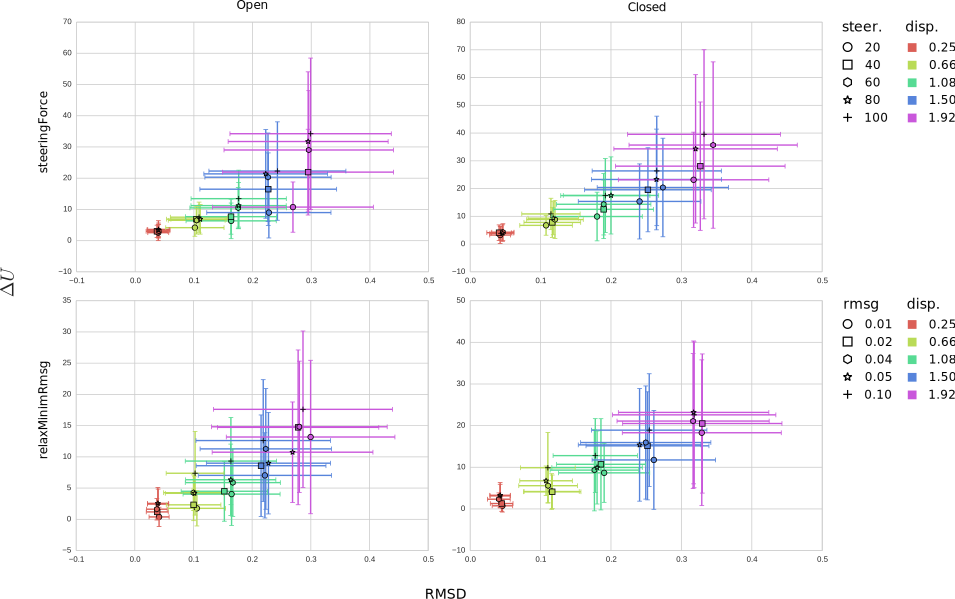
\includegraphics[width=\linewidth, height=\textheight, keepaspectratio]{CC_300_step_avg_rmsd_ener}
	\caption{Plot showing the relationship of the two studied parameters (\textit{steeringForce}  and \textit{MinimumRMS}) with the RMSD and energy increments of the Cartesian coordinate ANM step. Each point shows the average and standard deviation of the RMSD and energy increments for a given combination of parameters.}
	\label{fig:cc_300_avg_rmsd_energy}
\end{figure}

Having discarded to modify the \textit{steeringForce} parameter, we proceeded to perform other longer simulations (\around1500 steps) by varying the remaining parameters. Since the simulations starting from the closed structure looked more static, this time we started all simulations from the open structure. The reason for this behavior could be the higher overlap of the open conformation modes with the open to close transition. The simulations have been performed using temperatures between 300 K and 2568 K and the Spearman rank correlation for the (computational) step time, energy and RMSD increments (always of the NMA step) has been calculated (see Table \ref{tab:nma_correlations}).      

\begin{center}
\begin{longtable}{r r c c c c}


\toprule
~ & ~ & \multicolumn{2}{c}{CC} & \multicolumn{2}{c}{IC}\\
T & ~ & $\rho$ & p-value & $\rho$ & p-value \\
\midrule

300 & RMSD {\textbackslash} $\Delta U$ &  
\strcolor{0.79} &
$<$0.001 &
 \strcolor{0.69} &
$<$0.001\\
 &
Step time {\textbackslash} Displacement &
 \strcolor{0.563} &
$<$0.001 &
 \strcolor{0.615} &
$<$0.001\\
 &
Step time {\textbackslash} Relax. strength &
 \strcolor{-0.591} &
$<$0.001 &
 \strcolor{0.002} &
 0.783\\
 &
RMSD {\textbackslash} Displacement &
 \strcolor{0.786} &
$<$0.001 &
 \strcolor{0.78} &
$<$0.001\\
 &
RMSD {\textbackslash} Relax. strength &
 \strcolor{-0.057} &
$<$0.001 &
 \strcolor{-0.003} &
 0.594\\
 &
$\Delta U$ {\textbackslash} Displacement &
 \strcolor{0.656} &
$<$0.001 &
 \strcolor{0.717} &
$<$0.001\\
 &
$\Delta U$ {\textbackslash} Relax. strength &
 \strcolor{0.214} &
$<$0.001 &
 \strcolor{-0.005} &
 0.405\\
 \hline
 583 &
RMSD {\textbackslash} $\Delta U$ &
 \strcolor{0.79} &
$<$0.001 &
 \strcolor{0.63} &
$<$0.001\\
 &
Step time {\textbackslash} Displacement &
 \strcolor{0.548} &
$<$0.001 &
 \strcolor{0.591} &
$<$0.001\\
 &
Step time {\textbackslash} Relax. strength &
\strcolor{-0.598} &
$<$0.001 &
 \strcolor{-0.006} &
 0.274\\
 &
RMSD {\textbackslash} Displacement &
 \strcolor{0.803} &
$<$0.001 &
 \strcolor{0.785} &
$<$0.001\\
 &
RMSD {\textbackslash} Relax. strength &
 \strcolor{-0.051} &
$<$0.001 &
 \strcolor{0.001} &
 0.895\\
 &
$\Delta U$ {\textbackslash} Displacement &
\strcolor{ 0.66} &
$<$0.001 &
 \strcolor{0.659} &
$<$0.001\\
 &
$\Delta U$ {\textbackslash} Relax. strength &
 \strcolor{0.213} &
$<$0.001 &
 \strcolor{0.007} &
 0.216\\
\midrule
 866 &
RMSD {\textbackslash} $\Delta U$ &
 \strcolor{0.79} &
$<$0.001 &
 \strcolor{0.6} &
$<$0.001\\
 &
Step time {\textbackslash} Displacement &
 \strcolor{0.562} &
$<$0.001 &
 \strcolor{0.588} &
$<$0.001\\
 &
Step time {\textbackslash} Relax. strength &
 \strcolor{-0.605} &
$<$0.001 &
 \strcolor{0.001} &
 0.808\\
 &
RMSD {\textbackslash} Displacement &
 \strcolor{0.794} &
$<$0.001 &
 \strcolor{0.788} &
$<$0.001\\
 &
RMSD {\textbackslash} Relax. strength &
 \strcolor{-0.03} &
$<$0.001 &
 \strcolor{-0.005} &
 0.374\\
 &
$\Delta U$ {\textbackslash} Displacement &
 \strcolor{0.656} &
$<$0.001 &
 \strcolor{0.629} &
$<$0.001\\
 &
$\Delta U$ {\textbackslash} Relax. strength &
 \strcolor{0.195} &
$<$0.001 &
 \strcolor{0.011} &
 0.059\\
\midrule
 1150 &
RMSD {\textbackslash} $\Delta U$ &
 \strcolor{0.79} &
$<$0.001 &
 \strcolor{0.58} &
$<$0.001\\
 &
Step time {\textbackslash} Displacement &
 \strcolor{0.569} &
$<$0.001 &
 \strcolor{0.618} &
$<$0.001\\
 &
Step time {\textbackslash} Relax. strength &
 \strcolor{-0.579} &
$<$0.001 &
 \strcolor{0.002} &
 0.753\\
 &
RMSD {\textbackslash} Displacement &
 \strcolor{0.799} &
$<$0.001 &
 \strcolor{0.79} &
$<$0.001\\
 &
RMSD {\textbackslash} Relax. strength &
 \strcolor{-0.033} &
$<$0.001 &
 \strcolor{0.005} &
 0.372\\
 &
$\Delta U$ {\textbackslash} Displacement &
 \strcolor{0.65} &
$<$0.001 &
 \strcolor{0.607} &
$<$0.001\\
 &
$\Delta U$ {\textbackslash} Relax. strength &
 \strcolor{0.182} &
$<$0.001 &
 \strcolor{0.003} &
 0.603\\
\midrule
 1432 &
RMSD {\textbackslash} $\Delta U$ &
 \strcolor{0.79} &
$<$0.001 &
 \strcolor{0.56} &
$<$0.001\\
 &
Step time {\textbackslash} Displacement &
 \strcolor{0.543} &
$<$0.001 &
 \strcolor{0.579} &
$<$0.001\\
 &
Step time {\textbackslash} Relax. strength &
 \strcolor{-0.609} &
$<$0.001 &
 \strcolor{-0.016} &
 0.006\\
 &
RMSD {\textbackslash} Displacement &
 \strcolor{0.787} &
$<$0.001 &
 \strcolor{0.79} &
$<$0.001\\
 &
RMSD {\textbackslash} Relax. strength &
 \strcolor{-0.046} &
$<$0.001 &
 \strcolor{-0.005} &
 0.38\\
 &
$\Delta U$ {\textbackslash} Displacement &
 \strcolor{0.656} &
$<$0.001 &
 \strcolor{0.589} &
$<$0.001\\
 &
$\Delta U$ {\textbackslash} Relax. strength &
 \strcolor{0.187} &
$<$0.001 &
 \strcolor{0.001} &
 0.822\\
\midrule
 2000 &
RMSD {\textbackslash} $\Delta U$ &
 \strcolor{0.75} &
$<$0.001 &
 \strcolor{0.53} &
$<$0.001\\
 &
Step time {\textbackslash} Displacement &
 \strcolor{0.563} &
$<$0.001 &
 \strcolor{0.559} &
$<$0.001\\
 &
Step time {\textbackslash} Relax. strength &
 \strcolor{-0.566} &
$<$0.001 &
 \strcolor{0.003} &
 0.608\\
 &
RMSD {\textbackslash} Displacement &
 \strcolor{0.782} &
$<$0.001 &
 \strcolor{0.791} &
$<$0.001\\
 &
RMSD {\textbackslash} Relax. strength &
 \strcolor{-0.044} &
$<$0.001 &
 \strcolor{0.001} &
 0.884\\
 &
$\Delta U$ {\textbackslash} Displacement &
 \strcolor{0.615} &
$<$0.001 &
 \strcolor{0.561} &
$<$0.001\\
 &
$\Delta U$ {\textbackslash} Relax. strength &
 \strcolor{0.198} &
$<$0.001 &
 \strcolor{0.008} &
 0.169\\
\midrule
 2568 &
RMSD {\textbackslash} $\Delta U$ &
 \strcolor{0.75} &
$<$0.001 &
 \strcolor{0.51} &
$<$0.001\\
 &
Step time {\textbackslash} Displacement &
 \strcolor{0.57} &
$<$0.001 &
 \strcolor{0.395} &
$<$0.001\\
 &
Step time {\textbackslash} Relax. strength &
 \strcolor{-0.556} &
$<$0.001 &
 \strcolor{-0.046} &
$<$0.001\\
 &
RMSD {\textbackslash} Displacement &
 \strcolor{0.784} &
$<$0.001 &
 \strcolor{0.792} &
$<$0.001\\
 &
RMSD {\textbackslash} Relax. strength &
 \strcolor{-0.047} &
$<$0.001 &
 \strcolor{0.002} &
 0.707\\
 &
$\Delta U$ {\textbackslash} Displacement &
 \strcolor{0.598} &
$<$0.001 &
 \strcolor{0.53} &
$<$0.001\\
 &
$\Delta U$ {\textbackslash} Relax. strength &
 \strcolor{0.199} &
$<$0.001 &
 \strcolor{-0.003} &
 0.547\\
\bottomrule

\caption{Association strenght of the RSMD and energy increments, and step time between themselves and the chosen parameters. }\\
\label{tab:nma_correlations}\\

\end{longtable}

\end{center}

The results show a strong association between the RMSD increment and the energy increment. This is somewhat expected, as big deformations can, in the CC case, distort the topology and, in the IC case, produce more steric clashes. It is remarkable, however, that the association strength is always smaller for the icNMA step, supporting our hypothesis that the icNMA method is able to deform the protein producing smaller energy increments. In this last case we see a slight anticorrelation with the temperature. This is surprising, since all these measures have been taken inside the NMA step and, thus, may be independent of the temperature. 
%\hl{Possible hypotheses for this are: faster sampling of non harmonic regions, or the appearance of multiple pathways, etc., which are associated to a smoother energy landscape in the IC representation.}  

RMSD increments have a strong association with the displacement magnitude, as expected, and no association with relaxation strength in both cases. The energy increment during the NMA step and the displacement magnitude are strongly associated, the explanation behind this is the same that relates RMSD and energy increment. Energy increment and relaxation strength have a loose association in the ccNMA method. This relationship does not exist in the IC case, showing that early convergence should be enough to get rid of steric clashes. All these measures seem to be independent of the temperature.
 
The computational time needed to fulfil the NMA step is, in both cases, strongly related to the displacement magnitude. The reasons are different for each method: In the ccNMA step, the more distant the target positions are, the more difficult the convergence of the minimization becomes, as it has to fulfill the force field constraints plus the ANM constraints. In the icNMA case, the wider the rotation is, the easier it is to generate steric clashes, which are harder to relieve using the minimization. 

Finally, we can observe that the computational time the ccNMA needs to perform a step is also strongly associated with the ANM minimization strength, while this association is almost nonexistent in the IC case, giving us more freedom to change the value of this parameter without time penalties.  

\subsection{Obtention of the best simulations and comparison with MD}
One of the goals of this project is to evaluate to which extent the icNMA implementation improves PELE sampling capabilities. To this end, we have decided to compare simulations using both methods with a third reference method: MD. We have tested two different systems, ubiquitin (PDB id: 1UBQ) a small and very static globular protein,  and a c-Src kinase (PDB id: 1Y57) as an example of a bigger and more flexible protein.

\subsubsection{Best values for the parameters at 300 K} 
The value of the parameters used in a simulation can dramatically alter its outcome. As the icNMA-based method is new, and the ccNMA-based method is not  commonly used at 300, we do not have a predefined set of default values for the parameters to use in the simulations. As a consequence, we have worked to obtain the best parameterizations in order to make the comparison fairer. Here, we will illustrate the procedure we followed for the parameterization of the c-Src kinase simulation.
 
First, we have fixed the parameters common to both methods e.g. the temperature was set to 300 K and the distance cutoff for the construction of the EN was set to 9 \angstrom. Then, using the simulations we had already run with the parameters detailed in Table \ref{tab:parameters}, we have calculated the values of the three indices we were going to use to discriminate the best values for the parameters: 

\begin{itemize}
\item The average RMSD increment of the ANM step, which gives us an idea of the extent of the deformations.
\item The root mean square of the root mean square fluctuations (RMSF) for each simulation vs. the RMSF of the MD simulation. This can tell us if the flexibility of our simulations resemble that of the MD simulations.
\item The acceptance, which we wanted to keep in the 20-40\% range.  
\end{itemize}

After applying the acceptance restriction, the list of possible parameterizations went down to three possibilities for each of the simulations (see Table \ref{tab:nma_sim_parameters}) and we were able to choose a good set of parameters for the regular PELE simulations: 0.66 \angstrom for the \textit{displacementFactor} parameter and 0.1 for the \textit{MinimumRMS} parameter. Note that, as results are so similar, we decided to select the higher value of \textit{MinimumRMS}, as we knew it would shorten the execution time of each step. 

For the icNMA method, we saw a high difference in acceptance between the simulations with \textit{displacementFactor} equal to 0.05 rad and \textit{displacementFactor} equal to 0.08 rad, indicating that our angular step choice was too big. To verify this, we refined the icNMA simulations using values of the \textit{displacementFactor} between 0.05 rad and 0.08 rad. The optimum value turned to be around the 0.065 rad. As the method uses a maximum and minimum value for the rotations, we performed further tests using values around 0.065 rad. as the lower limit and an arbitrary maximum value of 0.02 rad. The best combination we found was the range from 0.07 rad to 0.14 rad. 

\begin{table}
\centering
\begin{tabular}{r c c c c c}
\toprule
~ & Acceptance & RMS(RMSF) & RMSD & Disp. mag. (\angstrom) & Rel. str.\\
\midrule
CC & 0.316 & 2.467 & 0.094 & 0.66 &0.05\\
~ & 0.308 & 2.492 & 0.098 & 0.66 &0.01\\
~ & 0.281 & 2.447 & 0.09 & 0.66 &0.1\\
\midrule
IC & 0.334 & 2.618 & 0.126 & 0.5 &0.05\\
~ & 0.328 & 2.642 & 0.127 & 0.5 &0.1\\
~ & 0.298 & 2.651 & 0.126 & 0.5 &0.01\\
\midrule
IC & 0.296 & 2.637 & 0.139 & 0.55 &0.1\\
(refinement) & 0.295 & 2.639 & 0.137 & 0.55 &0.05\\
~ & 0.29 & 2.635 & 0.138 & 0.55 &0.01\\
~ & 0.284 & 2.629 & 0.148 & 0.6  &0.1\\
~ & 0.264 & 2.63 & 0.149 & 0.6  &0.01\\
~ & 0.26 & 2.588 & 0.165 & 0.65 &0.05\\
~ & 0.249 & 2.608 & 0.168 & 0.65 &0.01\\
~ & 0.248 & 2.614 & 0.153 & 0.6  &0.05\\
~ & 0.245 & 2.612 & 0.164 & 0.65 &0.1\\
~ & 0.229 & 2.592 & 0.179 & 0.7  &0.01\\
\bottomrule
\end{tabular}


\caption{Values for the parameters that produced simulations with acceptance between 20 and 40\%.}
\label{tab:nma_sim_parameters}
\end{table}

Once we got the best parameter choice for the icNMA step, we still needed to parameterize the rotation amplitude range of the side chain perturbation step. To this end, we performed several simulations using different values for the maximum and minimum rotation and choosing those which yield acceptance values between 20 and 40\%. The optimum range happened to be 0.02 to 0.024 radians.

\section{Comparison with MD}
We performed 12 independent 24 h simulations for each method and compared different measurements with MD. These measurements include:

\begin{description}

\item [Energy increments]
The increments of the potential energy due to the NMA step perturbation.  

\item [SASA and radius of gyration]
The SASA measures the area of the protein accessible to the solvent, while the radius of gyration calculates the dispersion of the atoms to its center of mass. Both measurements are related to the compactness of the protein.

\item [RMSF]
The RMSF is a measure of the fluctuation per residue (\calpha atom). We expect that similar methods produce similar conformational ensembles and, therefore, similar RMSF profiles. However, it is not guaranteed that two different conformational ensembles have different RMSF profiles. That is why we must combine this measure with others in order to have a real picture of the ensembles/methods similarity.      

\item [Conformational space overlap]
We used a similar approach to the ones shown by Lyman \textit{et al.} \cite{lyman_ensemble-based_2006} and Lindorff-Larsen \cite{lindorff-larsen_similarity_2009} to calculate the extension of the exploration in the conformational space overlap. This strategy consists in clustering the structures of all the methods together using a geometrical distance measure (RMSD). Then the square root of the Jensen-Shannon divergence of the cluster populations (converted to a probability distribution) is calculated, yielding the desired overlap value.
\end{description}

\subsection{Advantages of the new method}
We have observed that the ccNMA step is not able to generate energetically favorable proposals, i.e. proposals that maintain or lower the potential energy and thus will be accepted by means of a Boltzmann criterion. This is, indeed, the reason that makes the relaxation phase a necessary part of the PELE approach. The icNMA algorithm, however, is able to generate energetically favorable proposals \around18-27\% of the times and therefore does not need the computationally costly relaxation step. As a consequence, the icNMA-based algorithm is able to generate MC proposals faster than the ccNMA approach (\around5-7x), while keeping similar RMSD increments.   

The measurements of the SASA and radius of gyration for both algorithms reveal a tendency towards generating more compact structures than MD. This is not unexpected, as our methods use implicit solvent, which is known to produce a bias in favor of compact structures \cite{onufriev_exploring_2004, chen_implicit_2008, zhang_residual_2012}, while our reference MD simulations were run in explicit solvent. There is a remarkable difference between the results for icNMA and ccNMA, being the former in better accordance with MD. The increased compaction of the ccNMA-based algorithm seems to be caused by the repeatedly use of minimizations, which enforce the solvent bias. The absence of backbone minimizations in the icNMA method limits the severity of the bias.  

We also studied the relative fluctuations of the residues by scaling the RMSF profiles and superimposing them. The RMSF profiles of the icNMA method show, in general, good agreement with MD. The ccNMA method shows a poorer performance in the ubiquitin case, specially in the $\beta2$-$\alpha$-helix and the $\beta$4-$\beta$5 loop regions. 

The study of the conformational space overlap shows that, in general, the icNMA-based method is populating regions of the conformational space closer to MD than to the ccNMA-method. Besides, we performed additional analyses of the sampling of the c-Src kinase P-loop. Correctly sampling this loop is of crucial importance as it is involved in the binding mechanisms of the kinase \cite{boggon_structure_2004}. We measured the distances between the atoms CYS:277:CA and LEU:387:CA, which is related to the inter-domain distance and the P-loop sampling. The icNMA algorithm is able to sample a similar range of distances to MD, however, ccNMA rapid compaction prevents it from obtaining similarly good results. This highlights the advantage of the icNMA method, which is less prone to get trapped in energy minima corresponding to compact structures.

\section[Limitations and perspectives]{Limitations of the new method and future perspectives}

In general, we observed that the RMSF baselines of the NMA-based methodologies is always lower  MD baselines. This points to the main limitations of the new method: the lack of anharmonic backbone movements and mapping higher (local) frequency modes, which reduces the amplitude of fluctuations. We wonder if this could be overcome by using IC Principal Component Analysis (PCA) modes, which are known to have a higher anharmonic component \cite{hayward_harmonic_1994}. Also, both methods show high RMSD differences with the structures coming from the MD trajectories. This differences are more evident in the ubiquitin case, where the flexibility of the protein is concentrated on the loops connecting the secondary structure. The cause of these RMSD differences reflects, indeed, the inability of our set of low-frequency NMA modes to model the high-frequency movements occurring in these loops. 

We are currently working to yet lower the execution times and keep improving the simulation flexibility. Our aim is to make this method a good alternative to current VHTS software by finding a good trade off between simulation detail and speed. Moreover, by coupling this procedure with a ligand perturbation step, as done in the PELE algorithm, local fluctuations (not present in the NMA) can be recovered through the response of the protein to the ligand move. We believe that the improvements in simulation reliability shown here can suppose a gain in the long term. Although it is true that it involves a considerable increase in the calculation times, it can save time (and money) at a later stage of the drug discovery process by the early elimination of false positives and negatives.

\newpage

\newpage
\cleardoublepage
\section[Efficient and reliable analysis]{Efficient and reliable analysis of huge conformational ensembles}

In the computational biology field,  the evolution of hardware during the last decade has allowed tools to run faster, thus making them able to produce larger output in the same amount of time. Nowadays, the efficient storage and analysis of these increasingly big results can become a problem.
 
This is indeed our case, since one of our objectives is the development of faster conformational sampling tools, capable of being applied in VHTS. That is why we have focused on the improvement of the efficiency and robustness of the analysis of large ensembles of biomolecular
structures.

\subsection{Efficient calculation of collective superimposition operations}

Collective superimposition operations are fundamental routines in structural biology related
analysis methods and can become a bottleneck if data sets are large. We have implemented an efficient alternative to performing these operations and RMSD calculations:
pyRMSD \cite{gil_pyrmsd_2013-1}. We have focused on three common use cases:

\begin{itemize}
\item Superimposition of a given conformation vs. the others in the ensemble (e.g. the first frame of a trajectory is usually
compared to the others in order to calculate an RMSD profile).
\item Pairwise superimposition of all the conformations of the ensemble. A pairwise superimposition of all conformations
of the ensemble would be necessary to build an RMSD matrix to be used by a clustering algorithm
\item Iterative superimposition of all the conformations of the ensemble. All conformations can be iteratively
superimposed before calculating the covariance matrix for a PCA. 
\end{itemize}
Python is an object-oriented interpreted language that seems to be currently gaining momentum among researchers. This may be due to the great availability of scientific libraries or to the possibility of creating software prototypes without effort. 

\begin{sidewaysfigure}

\fittopageimage{pyRMSD_uml}

\caption{ Pseudo-UML (Unified Modelling Language) diagram showing some key classes of pyRMSD as well as
the three-layer design (Python classes, Python C interface and C++ classes).}

\label{fig:pyrmsd_uml}

\end{sidewaysfigure}

\subsection{Superimposition algorithms}

pyRMSD has been designed as a Python library implementing a three-layer structure (see Fig.
\ref{fig:pyrmsd_uml}). The first layer is written in pure Python and contains high-level objects and
functions. The second layer describes the C Python API interface, which links the low-level functions of the third layer
with the high-level functionalities of the first one. The third layer is a full C++ library implementing the
superimposition and RMSD calculation functions. Thanks to this structure, pyRMSD can be included effortlessly in other
Python or C++ projects, ensuring the reuse of the code.



pyRMSD implements Kabsch's algorithm \cite{kabsch_solution_1976}, Heisterberg's algorithm (aka
QTRFIT) \cite{heisterberg_qtrfit_1990} and Theobald's algorithm (QCP)
\cite{theobald_rapid_2005-1}. These three methods try to solve the superimposition problem by
different means, but with the common goal of finding a rotation matrix (or equivalent quaternion) that minimizes the
error function:

\begin{equation}
e^2 = \frac{1}{n} \sum_n \left| x_n - U y_n \right| ^2 .
\end{equation}


The inclusion of these three algorithms in one package obeys two reasons: the need to compare algorithm performance, and the necessity to provide users with an alternative in case they need to overcome any of the problems associated with these algorithms (e.g. Kabsch's can potentially produce rotoreflection matrices \cite{umeyama_least-squares_1991} and QCP is known to have bad convergence).

\subsection{Parallelization and performance}

The core functions of the third layer have been parallelized in order to boost performance. All three algorithms have a
serial and OpenMP version to take advantage of multicore CPUs. In addition, QCP also implements a CUDA version that can run in Nvidia GPUs with both single and double floating point precision. This is has been the first open source CUDA implementation of this algorithm so far.

When testing the ``one conformation versus the others'' use case in a 30k snapshots trajectory, the faster algorithm showed a
\around2.6x speedup using OpenMP with six threads. Improvements are more noticeable when testing the calculations of RMSD
matrices, with speedups ranging from 5x (OpenMP) to 11x faster (CUDA using the ``in-memory matrix'' alternative). 

Furthermore, the comparison of pyRMSD with g\_rmsd \cite{berendsen_gromacs_1995}, a RMSD matrix
calculation specialized piece of software, shows that the former is more than four times faster. We have also implemented
several RMSD matrix calculation examples using non-specific software (see Supplementary materials S6 of the
publication). The best-performing function uses Prody, a well consolidated Python package, and  is 50x slower than
pyRMSD.

Our profilings have revealed that, when using distance matrices, the contribution of the matrix access time starts to become prominent if the superimposition bottleneck is eliminated. This behaviour can be explained based on Python's inherent overhead in array element access operations, e.g. Python checks internally that these indices are integers or that they are pointing to a legal position of the array. As these checks are an automatic part of the runtime, we needed to create the ``CondensedMatrix'' object. This is a C Python object that stores a square symmetric matrix in a memory efficient
way and bypasses indexing checks to decrease access overhead to almost zero, adding a 6x automatic speed up to any
function using it.

\subsection{Distribution}

pyRMSD is distributed as open source software and is maintained in a public GitHub
repository\footnote{\url{https://github.com/victor-gil-sepulveda/pyRMSD}}. It can be easily installed using customary
Python installation methods (setup.py and pip remote installation). We have also added a new makefile-like setup script
that allows defining different hardware parameters and environments so that users can make the most of their machine architectures. This installation script also overcomes some current  Python limitations related to CUDA code compilation.

\newpage




\newpage
\cleardoublepage
\section{A reliable cluster analysis protocol}

Cluster analysis is a powerful non-supervised analysis technique which aims to group the elements of a data set so
that its underlying structure gets unveiled. This allows discovering properties of data that would be impossible to
obtain through other means. 

It has been extensively used in several fields, and computational biology is not an exception. For instance, it is used in
population analysis of ensembles \cite{shao_clustering_2007}, to summarize simulation output
\cite{fraccalvieri_self_2013, phillips_validating_2011}, finding native-like structures in homology modeling refinement processes \cite{raval_refinement_2012} or as a key part of Markov State Model (MSM) analysis \cite{pande_everything_2010}.

\subsection{Looking for the best clustering}

The results of a cluster analysis heavily depend on the choice of the algorithm and its parameters (see Fig.
\ref{fig:pyproct_cluster_methods}). Cluster analysis is also very sensitive to the distance metric
used. It is known, for instance, that RMSD sensibility can make clustering more difficult, especially when structural
dissimilarity is high. Also, the so-called ``curse of dimensionality'' can suppose a problem here. Consequently, using
cluster analysis as a black box can be dangerous: as cluster analysis is usually part of other more complex analyses or
algorithms, erroneous partitions would directly compromise all derived results. 

\begin{figure}

\fittopageimage{clusterMethods}

\caption{Four cluster analysis have been performed over the same data set. Results can change
dramatically depending on the algorithm (k-medoids or spectral clustering here) and parameters used (k = 2 or k = 3).}

\label{fig:pyproct_cluster_methods}

\end{figure}

A cluster analysis algorithm is usually considered to be good if it is able to classify the data set so that each of
them is more similar to the elements of their own group than to the elements in the other groups. However, this
definition does not always apply. In Fig. \ref{fig:pyproct_cluster_methods} we have used two
algorithms and two parameter sets, thus obtaining four different clusterings. The two upper clusterings show perfect
equipartitions of the space; the two lower clusters are able to capture the circular shape to some extent. This leads to a question: which is the correct result? For instance, the first solution would be a good outcome if we embrace the definition above, while the second one would be especially useful in a computer vision scenario where the shape of objects must be identified. The best clustering is, indeed, the one that best fits the user's goals
\cite{luxburg_tutorial_2007}.

\subsection{pyProCT}

We have created pyProCT
\cite{gil_pyproct_2014-1} in order to have a robust cluster analysis method that can be used without understanding how cluster analysis algorithms work. The pyProCT work flux starts with users defining a working hypothesis by using their domain expertise and their knowledge about the problem they are facing. This hypothesis describes the results that they would consider useful using just a few
parameters, and obliges  them to identify the specific goals of their clustering efforts. For instance, a user trying to analyze an MD trajectory of a system he or she is studying may know the following: the approximate number of expected clusters, the expected size of populations, or whether the method is prone to produce ``noisy'' ensembles. 

The second part of the hypothesis is built around the definition of one or more scoring criteria. These are based on simple concepts, such as the degree of cluster separation or cohesion. The hypothesis will be used by pyProCT to perform a clustering exploration with five different clustering algorithms (K-means, Spectral clustering, DBSCAN, hierarchical complete linkage and GROMOS), and different sets of automatically generated parameters. Thanks to
the previously defined hypothesis and scoring criteria, the software will choose the result that better fulfills the user's expectations.

\subsection{Hypothesis refinement}

It is very likely that the first hypothesis does not  define the user's goals completely. Users may gain knowledge from result inspection, and this knowledge can be used to refine the hypothesis and the cluster again. Although this step is not mandatory, the preferred and more reliable way of working with pyProCT is performing these iterative hypothesis refinement cycles.

\subsection{Software flow detail}

We have implemented pyProCT as a flow of 5 stages: 

\begin{enumerate}
\item Distance matrix calculation. All clustering algorithms need to calculate the distances (or similarities) of the
elements in the data set. In the case of protein conformations, this calculation implies a costly superimposition. Therefore, precalculating the distances can be advantageous as the superimposition step can be time-consuming. pyProCT allows the use of RMSD and Euclidean distances. RMSD is calculated using pyRMSD and extends it by adding a way to
define groups with symmetries, as well as automatic matching of symmetric chains in oligomers in order to obtain
the minimum RMSD value every time. The Euclidean distance option calculates distances between the center of mass of the selected
groups.
\item Algorithm parameterization. A set of parameters is calculated using a different methodology for each algorithm
based on the working hypothesis.
\item Cluster analysis. All the algorithms (or a user-defined subset) are used in combination with the parameterizations
found in the previous stage. This produces an ensemble of clustering solutions that will be filtered in order to avoid
repetitions and solutions that do not agree with the user's hypothesis. 
\item Remaining clusterings are scored using both hypothesis and the defined scoring criteria.
\item The best result is chosen and analyzed
\end{enumerate}
pyProCT can take advantage of parallel architectures thanks to pyRMSD. As the workflow is composed of well-defined
independent tasks, it has been possible to parallelize it using a naive parallelization scheme. A scheduler has been
added so that tasks can be distributed to more than one processor (at node level, using native Python parallel functions)
or more than one node (at cluster level, using MPI). A new scheduler type using pyCOMPSs
\cite{tejedor_pycompss_2015} has  recently been developed
\cite{alvarez_vecino_optimization_2015}. pyCOMPSs is an annotation-based parallel programming model
for Python based on COMPSs \cite{tejedor_high-productivity_2012}. The inclusion of this scheduler
improves the load balance and opens the door to the execution of pyProCT in cloud architectures. 

\subsection{Scoring criteria}

A crucial step in the craft of the working hypothesis is the definition of the scoring criteria. Each scoring
criterion is a weighted sum of a set of clustering quality functions. Only internal clustering validation indices
(ICVs) have been used, such as the Silhouette index, Cohesion or Separation, as there is not a correct
clustering available to use as a reference. The implemented ICVs have been defined and discussed in Section \ref{sec:pyproct_supp_2}. 
By defining more than one criterion, users can prepare the analysis for more than one
scenario (e.g. the example in Section \ref{sec:pyproct_supp_6} uses one criterion that defines the common
description of cluster analysis and another criterion that defines it in terms of graph components). In this case, the scores
for each criterion will be normalized and the best clustering will be the one with the higher score for any of the
criteria.

\subsection{Use cases}

Two main use cases have been presented:

\begin{itemize}
\item Cluster analysis: We have used pyProCT to analyze two different synthetic conformational ensembles. 
Populations, representatives, and global and per-cluster RMSFs have been automatically extracted from these ensembles. We have also used
pyProCT to analyze a DNA-ligand simulation where ligands were  in the bulk of the solvent most of the time. We have allowed
pyProCT to treat them as noise, which lead us to obtain the clusters of the interaction sites. The clusters found were
in good agreement with the ones obtained using MSM analysis in a prior work
\cite{lucas_atomic_2014}. 
\item Redundancy elimination: Storing data, and especially conformational ensembles, is becoming an issue of concern. We
have introduced a method that is able to eliminate redundant conformations while preserving ensemble cluster
populations. This makes it possible to process data sets whose distance matrix can not be fitted in memory. We have
tested it with a \around 100,000 elements trajectory and a \around 1,000,000 elements ensembles with good results (see Section 3.2
 of the article, and Section \ref{sec:pyproct_supp_5} for more information). The method works by iteratively
partitioning the data set, cluster analyzing the partitions order to eliminate redundancy, and merging the results, until the
desired number of frames is reached. 
\end{itemize}


\subsection{Graphical User Interface (GUI)}

pyProCT includes a wizard-like html-based GUI that can assist users in order to generate a correct execution script,
launch pyProCT executions and visualize results. The result viewer processes pyProCT's result files and shows them in a
more understandable way making it a very useful tool for hypothesis refinement. 

\subsection{Distribution}

pyProCT is a Python standalone program that can also be integrated into other projects as a library. It is distributed
as open source software and is maintained in a public GitHub
repository\footnote{\url{https://github.com/victor-gil-sepulveda/pyProCT}}. It supports the setup.py installation
method and can also be installed using the pip package manager (which is the most convenient way of installing it as it
handles package dependencies automatically). pyProCT is far from being finished; code refactorings and new features
are included regularly (e.g. it has recently been upgraded to use numeric data sets).

\newpage

\newpage
\cleardoublepage

\newpage

\chapter{Conclusions}

\section{Technical improvement of PELE}
\begin{itemize}
\item[--] We have succeeded in implementing all the core functionalities of PELE using C++. The use of modern software engineering techniques has allowed us to better organize the code base and to introduce a test subsystem. Nowadays, PELE++ has become a piece of software which is easier to modify, understand, and extend. It is also more robust and reliable. The rewriting the code has helped us to overcome some of its previous technical limitations, such as the restrictions on the size of the systems. Also, it has allowed us to extend PELE with new solvent models, force fields, and types of biomolecules.
\item[--] The rewriting has make it possible to adapt the code in order to take advantage of new parallel architectures and accelerators. The parallelization of the non-covalent interactions and solvent model related functions, which represent hot spots in our performance analyses, has yielded promising speedup results. These new pieces of code are currently being integrated in PELE++.   
\item[--] PELE++ is, nowadays, the first choice for our research group. The new code has opened the doors to more ambitious developments involving machine learning and virtual reality. Also, a GUI for PELE++ is currently being created. 
\item[--] PELE++ has seriously been considered for pharmaceutical R\&D, which illustrates the success of the project. As a matter of fact, it is currently being tested in the Department of Medicinal Chemistry of the renowned pharmaceutical company AstraZeneca. 
\end{itemize}


\section{Algorithmic improvement of PELE}
\begin{itemize}
\item[--] We have proposed a new method using torsional normal mode analysis to improve the conformational sampling of PELE. We have found that internal coordinates normal modes are more collective and robust to the changes of the elastic network.  
\item[--] The method is able to produce more energy favorable perturbations than the current ANM-based strategy. This allows us to run simulations at 300 K without the need of complex relaxation protocols. As a consequence, the overall computational performance of the sampling is significantly improved (\around5-7x). We are currently working on the methodology to yet lower the execution times and further improving the simulation of flexibility. Thanks to the new methodology, we are attaining a good trade-off between speed and detail that will turn PELE into a good alternative to current VHTS software.
\item[--] The new internal coordinates-based methodology is able to capture the flexibility of the backbone better than the old method. The relative magnitudes of these fluctuations correlate well with those of our (explicit solvent) MD reference simulations.
\item[--] The new method better preserves the volume of the protein during the simulation, thus overcoming the tendency of PELE to produce compact structures in certain situations. 
\item[--] Finally, the inter-domain movements of c-Src kinase obtained with this method are closer to those obtained with MD.   
\end{itemize}

\section[Efficient and reliable analysis]{Efficient and reliable analysis of large conformational ensembles}
\begin{itemize}
\item[--] We have developed a Python package which is able to perform collective superposition (and RMSD) operations of conformational ensembles one order of magnitude faster than the serial version.  
\item[--] We have developed pyProCT, a cluster analysis software which is able to provide good results without any knowledge of cluster analysis techniques.
\item[--] pyProCT can be successfully used in the most common use cases: to retrieve clusters from ensembles of conformations (using RMSD) and to retrieve ligand clusters (using the distance to the center of mass). As requested by users, it isnow able to load and analyze other types of data, such as numeric arrays, allowing it to perform tasks beyond its original scope.  
\item[--] We also present a novel application to reduce the size of huge conformational ensembles by eliminating redundant structures. 
\item[--] pyProCT has already been used in a good number of biomedical publications for the analysis of results. It is currently being applied to improve PELE ligand sampling performance. Besides, it has been used in a Partnership for Advanced Computing in Europe (PRACE) project aiming at finding innovative ways to visually represent clusters of protein conformations.
\item[--] The code and compiled versions of both packages are available to the whole scientific community in free-access repositories. 
\end{itemize}



% ANM: When we use NMA-based methods, we are narrowing this search space to the reduced space of modes.mode selections. Must be weighted by freq.
%<Dani, futuro> Modes change if the ligand is docked or not in Diva (Djva) dos Santos et al JCTC 2012.
%<Kamiya> General internal coordinates. More than one molecule. Contributions of angles and bonds.

\newpage




\newpage

\makeatother
\printbibliography

\end{document}
